%----------------------------------------------------------------------------------------
%	PACKAGES AND THEMES
%----------------------------------------------------------------------------------------

\documentclass[aspectratio=169,9pt]{beamer}

\mode<presentation> {

  \usetheme{Boadilla} % light

  \usecolortheme{seahorse} % light

  %!TEX root = main.tex

\definecolor{CVUTBLUE}{RGB}{0,121,194}
\definecolor{CVUTBLUEDECREASED}{RGB}{0,141,204}
\definecolor{CVUTBLUEDECREASED2}{HTML}{bfcfe4}

\setbeamercolor{frametitle}{fg=white,bg=CVUTBLUE}

\setbeamertemplate{itemize items}[circle]
\setbeamercolor{itemize item}{fg=CVUTBLUE}

\setbeamercolor{section in head/foot}{bg=CVUTBLUE!0!black,fg=CVUTBLUE}
\setbeamercolor{institute in head/foot}{fg=CVUTBLUE}

\setbeamercolor*{palette primary}{fg=white,bg=CVUTBLUE}
\setbeamercolor*{palette secondary}{fg=white,bg=CVUTBLUEDECREASED}
\setbeamercolor*{palette tertiary}{fg=white,bg=CVUTBLUE}
\setbeamercolor*{palette quaternary}{fg=white,bg=black}
\setbeamercolor*{palette quinary}{fg=white,bg=CVUTBLUE}
\setbeamercolor*{palette senary}{fg=CUBlue,bg=white}

\setbeamercolor{title}{fg=white,bg=CVUTBLUE}

\setbeamercolor{block title}{fg=black,bg=CVUTBLUEDECREASED2}
\setbeamercolor{block body}{fg=black,bg=white}

%\definecolor{cblue}{RGB}{0,121,194}
%\def\blb{\color{cblue}\bf }

\setbeamertemplate{frametitle}
{
    \nointerlineskip
    \begin{beamercolorbox}[sep=0.0cm,ht=1.3em,wd=\paperwidth]{frametitle}%
        \vbox{}\vskip0.2ex%
        \hspace*{0.2em}\strut\insertframetitle\strut
        \hfill
        \raisebox{-0.4ex}{
\includegraphics[width=3cm]{fig/logo_ctu_fee_mrs_white.png}}\hspace*{0.3ex}
        \vskip-0.2ex%
    \end{beamercolorbox}
}


  % \setbeamertemplate{footline} % remove the footer line
  % \setbeamertemplate{footline}[page number] % replace the footer line with simple numbers

  \setbeamertemplate{navigation symbols}{}
  \setbeamertemplate{bibliography item}{\insertbiblabel} % removing the navigation symbols

}

%%{ Docu HEAD

\usepackage{graphicx} % Allows including images
\usepackage{booktabs} % Allows the use of \toprule, \midrule and \bottomrule in tables
\usepackage{multimedia}
\newcommand{\superfill}{\vskip0pt plus 1filll}

\usepackage{isotope}
\usepackage{animate}

\usepackage[export]{adjustbox}

\usepackage{graphicx}
\usepackage{setspace}
\usepackage{epstopdf}
\usepackage{float}
\usepackage{multirow,tabularx,makecell}

\usepackage{pdfpcnotes}

\usefonttheme{professionalfonts}
\usepackage{amsmath,amsfonts,amssymb,bm}

\usepackage[backend=bibtex,defernumbers=true,style=ieee,sorting=none,sortcites=false]{biblatex}

\renewcommand*{\bibfont}{\normalfont\tiny}

% Print labelnumbers with suffixes, adjust secondary labelnumber 2/2
\DeclareFieldFormat{labelnumber}{%
  \ifkeyword{mine}
  {\ifkeyword{core}
  {{\number\numexpr#1}}%
  {{\number\numexpr#1}}%
  }%
  {#1}%
  }

  \DeclareCiteCommand{\tabcite}%[\mkbibbrackets]
  {\usebibmacro{cite:init}%
  \usebibmacro{prenote}}
  {\usebibmacro{citeindex}%
  \usebibmacro{cite:comp}}
  {}
  {\usebibmacro{cite:dump}%
  \usebibmacro{postnote}}

  % {{\number\numexpr#1-\value{bbx:primcount}}a}

  %%{ fullcite box

  \usepackage{tcolorbox}

  \definecolor{light-gray}{gray}{0.95}
  \newcommand{\fullciteinbox}[2]{%

    \DeclareCiteCommand{\fullcite}
    {\usebibmacro{prenote}}
    {\clearfield{addendum}%
    \clearfield{issn}%
    \usedriver
    {\defcounter{minnames}{6}%
    \defcounter{maxnames}{6}}
    {\thefield{entrytype}}}
    {\multicitedelim}
    {\usebibmacro{postnote}}

    %\vspace{3em}%
    %\raisebox{3em}[3em][3em]{%
    % \vspace{-0.2em}
    % \begin{tcolorbox}[width=\textwidth,colback={light-gray},title={}]%
    \begin{block}{}
      \begin{minipage}[t]{0.07\linewidth}%
        \raggedright%
        \scriptsize \cite{#1}%
      \end{minipage}%
      \begin{minipage}[t]{0.93\linewidth}%
        \scriptsize \fullcite{#1}%
        \ifx&#2&
        \else
        \\
        \url{#2}
        \fi
      \end{minipage}%
      % \end{tcolorbox}%
    \end{block}
    %}%
    \vspace{-0.3em}
    }%

    %%}

    \addbibresource{main.bib}

    \defbibenvironment{favoritebib}
  {\itemize}
    {\enditemize}
  {\item}
    \usepackage{siunitx}
    \DeclareSIUnit \parsec {pc}
    \DeclareSIUnit \electronvolt {eV}
    \DeclareSIUnit \pixel {px}
    \DeclareSIUnit \arcmin {arcmin}
    \DeclareSIUnit \erg {erg}
    \DeclareSIUnit \joul {J}
    \DeclareSIUnit \Bq {Bq}

    \usepackage{enumitem} % To enable enumerate with letters (a, b, c...)
    \newlist{alphalist}{enumerate}{1}
    \setlist[alphalist]{label=\alph*)}
    \setlist[itemize]{label=\textbullet}

    \usepackage{cellspace}
    \newcolumntype{D}{>{\hfill}N{3}{2}<{\hfill}}
    \newcommand*\cellspacelimit[2]{\setlength{\cellspacetoplimit}{#1}\setlength{\cellspacebottomlimit}{#2}}

    % figures
    \usepackage{wrapfig}
    % \usepackage[font={footnotesize}]{caption}
    \usepackage[font={small}]{caption}
    % \usepackage{subcaption}

    % subfloat
    \usepackage{subfig}
    % \usepackage[export]{adjustbox}

    \usepackage{color}
    \usepackage{url}

    %%{ tikz

    \usepackage{tikz}
    \usepackage{pgfplots}
    \pgfplotsset{compat=1.14}
    \usetikzlibrary{backgrounds,arrows,automata,shapes,positioning,calc,through,spy,shapes,shapes.geometric,shapes.multipart,fit,patterns,fadings}
    \pgfdeclarelayer{background}
    \pgfdeclarelayer{foreground}
    \pgfsetlayers{background,main,foreground}

    \tikzset{
  state/.style={
    rectangle,
    draw=black, very thick,
    minimum height=1.0em,
    text centered,
  },
  state_red/.style={
    rectangle,
    draw=black, very thick,
    minimum height=1.0em,
    text centered,
    fill=red,
  },
  state_focus/.style={
    rectangle,
    draw=black, very thick,
    minimum height=1.0em,
    text centered,
    fill=black!50,
  },
  smallstate/.style={
    rectangle,
    draw=black, very thick,
    minimum height=0.2em,
    text centered,
  },
  final_state/.style={
    rectangle,
    rounded corners,
    draw=black, very thick,
    minimum height=2em,
    text centered,
  },
  initial_state/.style={
    rectangle,
    double=white,
    double distance=1pt,
    inner sep=2pt,
    draw=black, very thick,
    minimum height=2em,
    text centered,
  },
  point/.style={
    circle,
    inner sep=0pt,
    minimum size=3pt,
    fill=red
  },
  adder/.style={
    circle,
    inner sep=2pt,
    minimum size=0.3in,
    draw=black, very thick,
    text centered
  },
  state_gray/.style={
    rectangle,
    draw=black, very thick,
    fill=gray!40,
    minimum height=1.0em,
    text centered,
    inner sep=0,
  },
  state_white/.style={
    rectangle,
    draw=black, very thick,
    fill=white,
    minimum height=1.0em,
    text centered,
    text=black,
    inner sep=0,
  },
  nothing/.style={
  },
  state_blue/.style={
    rectangle,
    draw=black, very thick,
    fill=blue!40,
    minimum height=1.0em,
    text centered,
    text=black,
    inner sep=0,
  },
  final_state/.style={
    rectangle,
    rounded corners,
    draw=black, very thick,
    minimum height=2em,
    text centered,
  },
  initial_state/.style={
    rectangle,
    double=white,
    double distance=1pt,
    inner sep=2pt,
    draw=black, very thick,
    minimum height=2em,
    text centered,
  },
  point/.style={
    circle,
    inner sep=0pt,
    minimum size=3pt,
    fill=red
  },
}


    \tikzset{
      imgletter/.style={
        rectangle,
        inner sep=2pt,
        rounded corners=.1em,
        text=black,
        minimum height=1em,
        text centered,
        fill=white,
        fill opacity=1.0,
        text opacity=1,
        anchor=south west,
      },
    }

    \usetikzlibrary{shapes.arrows,backgrounds,arrows,automata,shapes,positioning,calc,through}

%%{ ARROWS

\tikzset{
  myarrow/.style={
    draw,
    fill=orange,
    single arrow,
    minimum height=3.5ex,
    single arrow head extend=1ex
  }
}

\newcommand{\arrowup}{%
  \vspace{-0.8em}
  \tikz [baseline=-0.5ex]{\node [myarrow,rotate=90] {};}
  \vspace{-1.4em}
}

\newcommand{\arrowdown}{%
  \vspace{-0.8em}
  \tikz [baseline=-1ex]{\node [myarrow,rotate=-90] {};}
  \vspace{-1.5em}
}

\newcommand{\arrowright}{%
  \tikz [baseline=-1ex]{\node [myarrow,rotate=0] {};}
}

\newcommand{\arrowleft}{%
  \tikz [baseline=-1ex]{\node [myarrow,rotate=180] {};}
}

%%}

%%{ CHECKMARK

\def\checkmark{\tikz\fill[scale=0.4](0,.35) -- (.25,0) -- (1,.7) -- (.25,.15) -- cycle;}

%%}

\pgfdeclarelayer{background}
\pgfdeclarelayer{foreground}
\pgfsetlayers{background,main,foreground}

\tikzset{
  state/.style={
    rectangle,
    draw=black, very thick,
    minimum height=1.0em,
    text centered,
  },
  state_gray/.style={
    rectangle,
    draw=black, very thick,
    fill=gray!40,
    minimum height=1.0em,
    text centered,
  },
  state_white/.style={
    rectangle,
    draw=black, very thick,
    fill=white,
    minimum height=1.0em,
    text centered,
    text=black,
  },
  state_green/.style={
    rectangle,
    draw=black, very thick,
    fill=green!50,
    minimum height=1.0em,
    text centered,
    text=black,
  },
  state_red/.style={
    rectangle,
    draw=black, very thick,
    fill=red!70,
    minimum height=1.0em,
    text centered,
    text=black,
  },
  state_blue/.style={
    rectangle,
    draw=black, very thick,
    fill=blue!40,
    minimum height=1.0em,
    text centered,
    text=black,
  },
  final_state/.style={
    rectangle,
    rounded corners,
    draw=black, very thick,
    minimum height=2em,
    text centered,
  },
  initial_state/.style={
    rectangle,
    double=white,
    double distance=1pt,
    inner sep=2pt,
    draw=black, very thick,
    minimum height=2em,
    text centered,
  },
  point/.style={
    circle,
    inner sep=0pt,
    minimum size=3pt,
    fill=red
  },
  nothing/.style={
    rectangle,
    rounded corners,
    draw=white, very thick,
    minimum height=2em,
    inner sep=2pt,
    text centered,
  },
  }



    %%}

    \usepackage{pdfpc-movie}
    \newcommand{\mymovie}[3][]{\pdfpcmovie[#1]{#2}{#3}}
    % \newcommand{\mymovie}[3][]{\movie[#1]{#2}{#3}}

            %%{ CHECKMARK IN TIKZ

            \def\checkmark{\tikz\fill[scale=0.4](0,.35) -- (.25,0) -- (1,.7) -- (.25,.15) -- cycle;}

            %%}

    \newcommand{\strong}[1]{\textbf{#1}}
    \newcommand{\coord}[1]{\textbf{#1}}
    \newcommand{\norm}[1]{\left\lvert#1\right\rvert}
    \newcommand{\m}[1]{\ensuremath{\mathbf{#1}}}
    \newcommand\numberthis{\addtocounter{equation}{1}\tag{\theequation}}
    \newcommand{\corrected}[1]{{\color{black} {#1}}}
    % \newcommand{\comment}[1]{{\color{blue} {#1}}}
    \newcommand{\add}[1]{{\color{green} {#1}}}
    \newcommand{\todo}[1]{{\color{red} TODO {#1}}}
    \newcommand{\updated}[1]{{\color{blue} {#1}}}
    \newcommand{\reffig}[1]{Fig.~\ref{#1}}
    \newcommand{\refalg}[1]{Alg.~\ref{#1}}
    \newcommand{\refsec}[1]{Sec.~\ref{#1}}
    \newcommand{\reftab}[1]{Table~\ref{#1}}
    \newcommand{\real}{\mathbb{R}}
    \newcommand{\red}[1]{{\color{red} #1}}
    \newcommand{\minus}{\scalebox{0.75}[1.0]{$-$}}
    \newcommand{\plus}{\scalebox{0.8}[0.8]{$+$}}
    \newcommand{\figvspace}{\vspace{-1em}} % this may eventually do something, so far just a placeholder

    % \usepackage{pgf}
    % \logo{\pgfputat{\pgfxy(0,5)}{\pgfbox[right,base]{\includegraphics[height=0.8cm]{}}}}
    % \newcommand{\nologo}{\setbeamertemplate{logo}{}}

    % \usepackage{eso-pic}
    % \newcommand\AtPagemyUpperLeft[1]{\AtPageLowerLeft{\put(\LenToUnit{0.66\paperwidth},\LenToUnit{0.904\paperheight}){#1}}}
    % \AddToShipoutPictureFG{
    %   \AtPagemyUpperLeft{{
\includegraphics[height=0.85cm,keepaspectratio]{fig/logo_ctu_fee_mrs_blue.png}}}
    % }
    % \newcommand{\AddToShipoutPictureFG}{\setbeamertemplate{logo}{}}

    %%}

    %%{ TITLE PAGE


    \title[MRS UAV System]{MRS UAV System for Real-world Testing and Development with Multirotor Aerial Vehicles}
    \subtitle{From control theory to practical use}
    \author[Tomas Baca]{{Dr. Tomas Baca} \\
    }
    \institute[CTU in Prague] {
      \begin{small}
        Multi-Robot Systems group, Faculty of Electrical Engineering\\
        Czech Technical University in Prague
      \end{small}}

    \date[July 29th, 2025]{}

    \titlegraphic{
\includegraphics[width=5cm]{fig/logo_ctu_fee_mrs_blue.png}}

    \begin{document}

    \begin{frame}

      \titlepage % Print the title page as the first slide

    \end{frame}

    % \nologo

    %%}

\section{UAV Experimentation in MRS}

%%%{ kumar

%\begin{frame}
%\frametitle{Motivation --- Awesome multi-UAV videos}

%\begin{block}{2012, University of Pennsylvania, prof. Vijay Kumar}
%  \begin{center}
%    \mymovie[autostart,loop]{
%      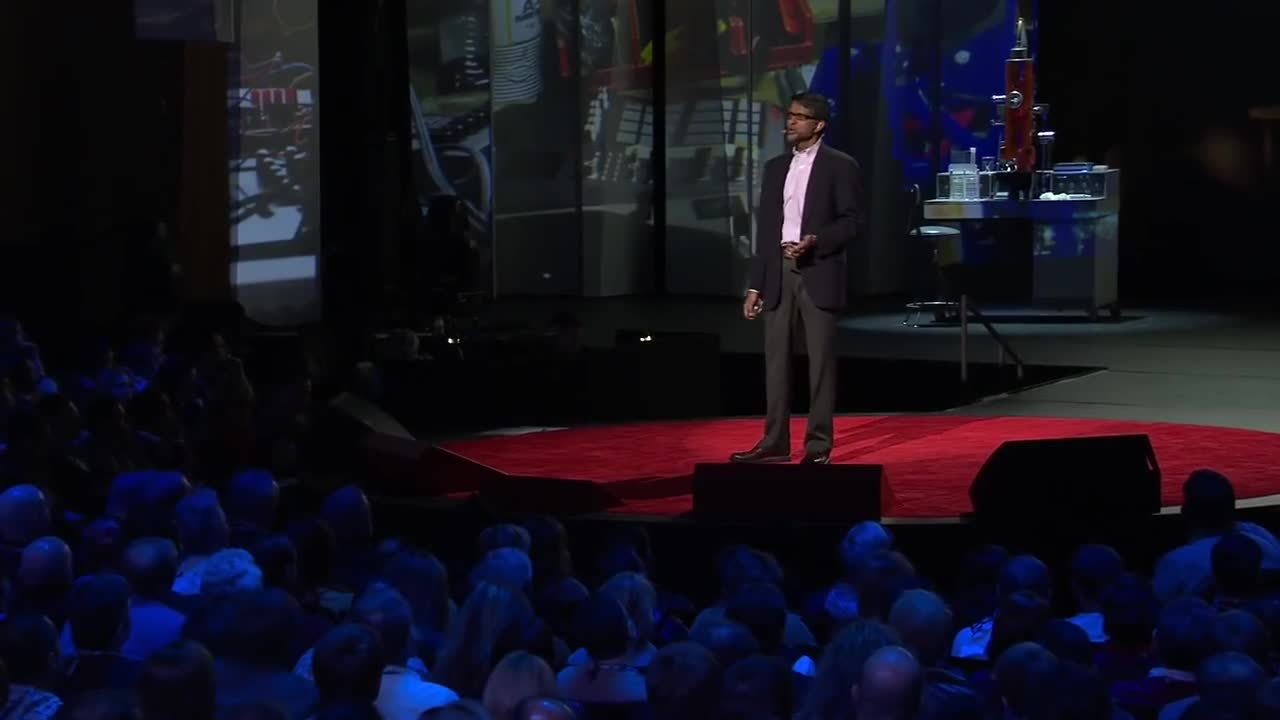
\includegraphics[width=0.7\textwidth]{./fig/kumar_thumbnail.jpg}
%    }{./videos/kumar.mp4}\\
%    Video: \url{https://youtu.be/4ErEBkj_3PY}
%  \end{center}
%\end{block}

%\end{frame}

%%%}

%%%{ UAV Experimentation in MRS

%\begin{frame}
%  \frametitle{UAV Experimentation in MRS (IMR) --- 2012--2016}

%  \vspace{-0.5em}

%  \only<+>{\begin{block}{$\approx$ 2012, designing custom PCBs for controllers}
%    \centering
%    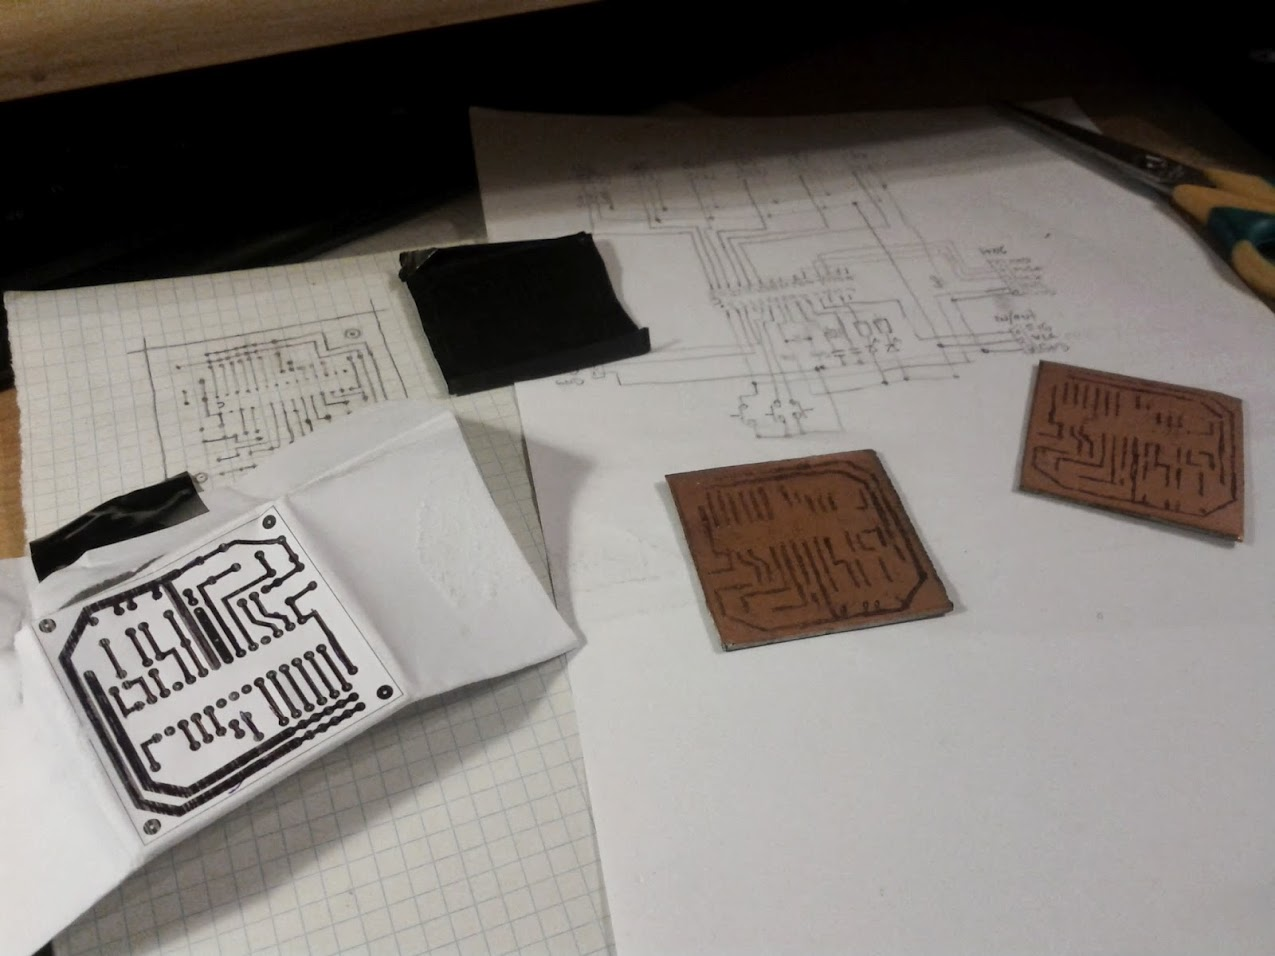
\includegraphics[width=0.48\textwidth]{fig/photos/pcb1.jpg}
%    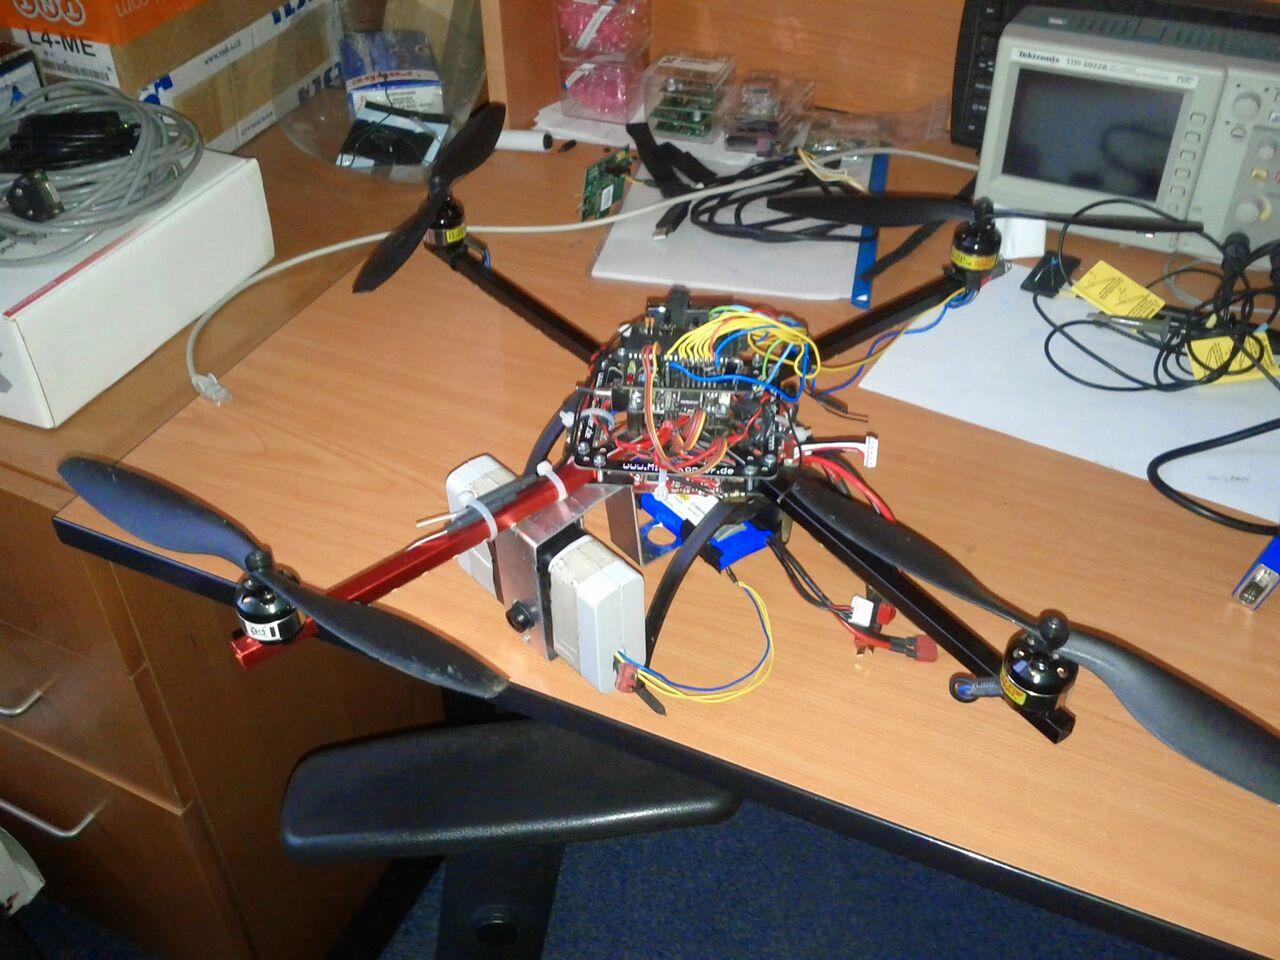
\includegraphics[width=0.48\textwidth]{fig/photos/first_UAV.jpg}
%  \end{block}}

%  \only<+>{\begin{block}{$\approx$ 2014, Model Predictive Control on embedded hardware}
%    \centering
%    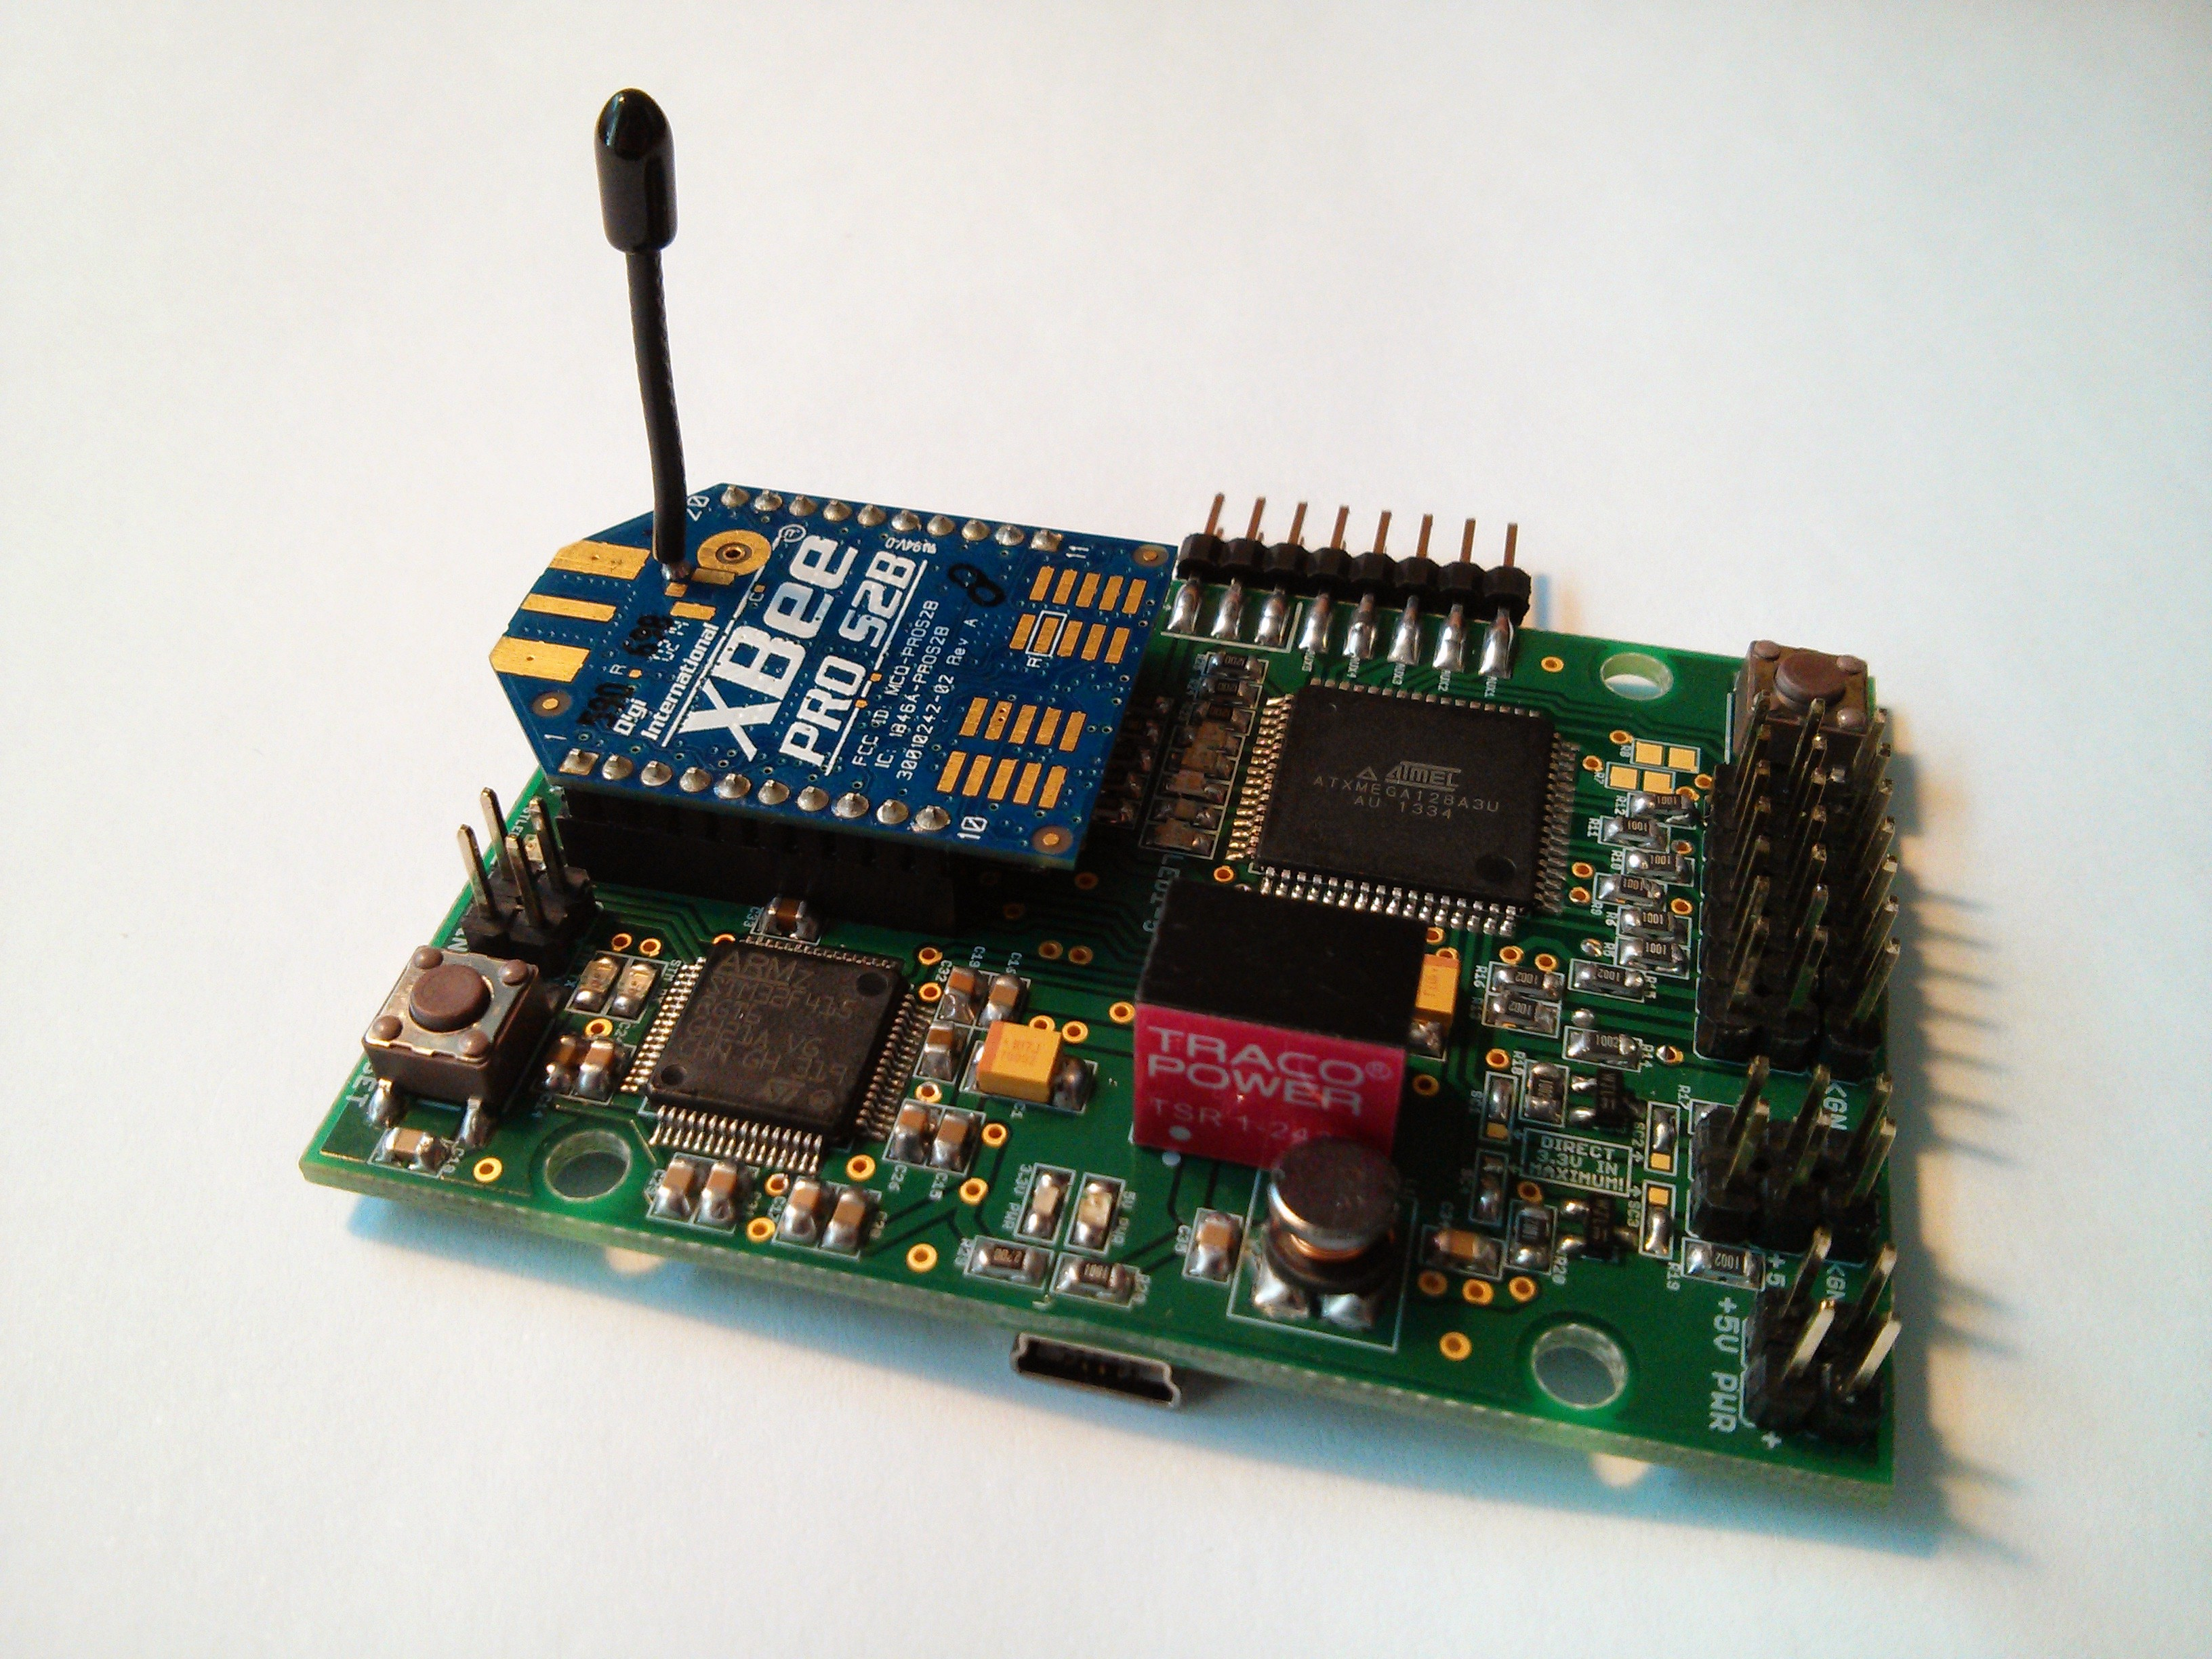
\includegraphics[width=0.48\textwidth]{fig/photos/pcb2.jpg}
%    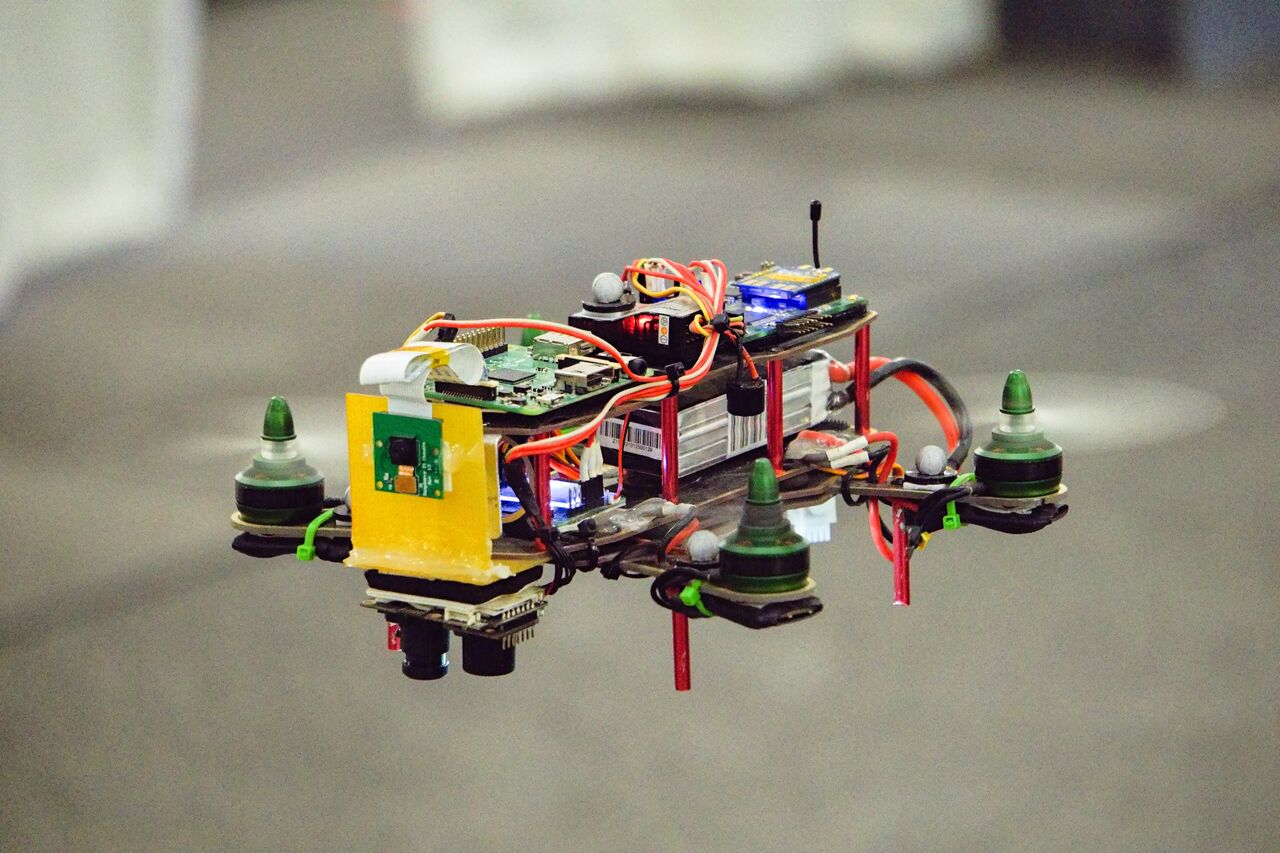
\includegraphics[width=0.48\textwidth]{fig/photos/prase.jpg}

%    \fullciteinbox{baca2016embedded}{}
%  \end{block}}

%  \only<+>{\begin{block}{Embedded Model Predictive Control}
%    \begin{center}

%      \mymovie[autostart,loop]{
%        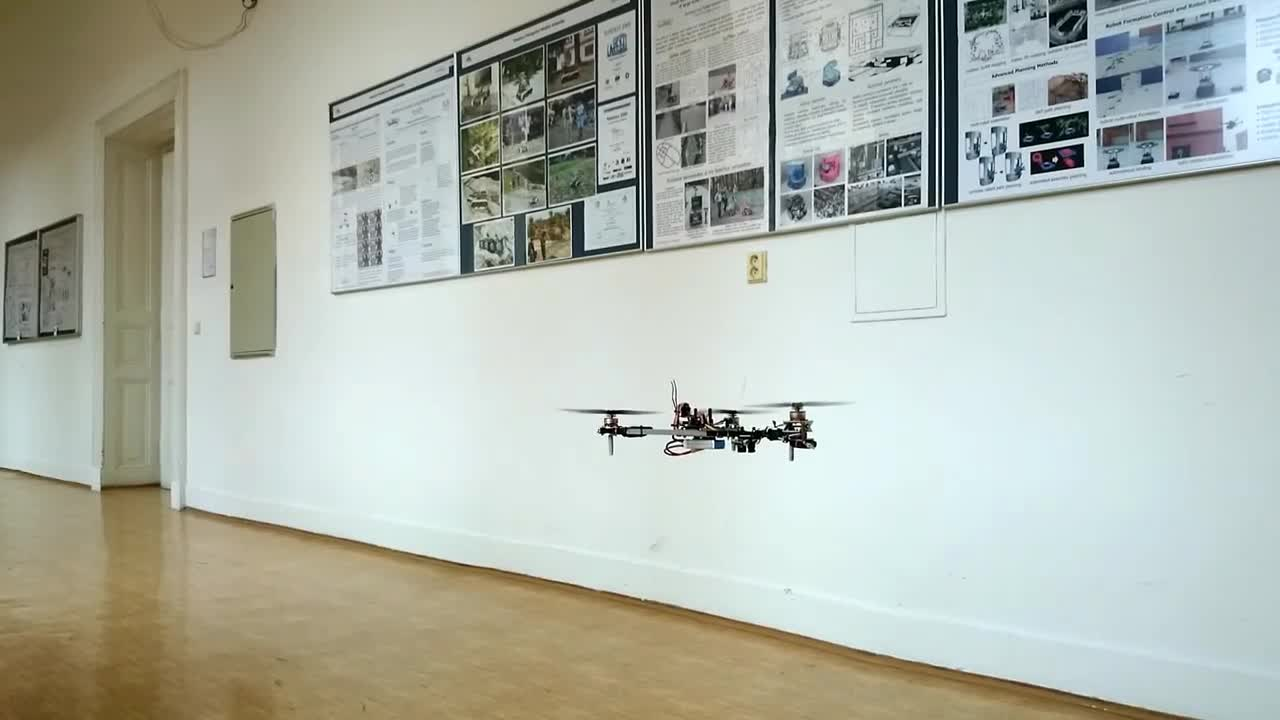
\includegraphics[width=0.7\textwidth]{fig/photos/embedded_mpc_thumbnail.jpg}
%      }{videos/embedded_mpc.mp4}\\
%      Video: \url{http://youtu.be/AXI_rkQRBaE}

%    \end{center}
%  \end{block}}

%  \only<+>{\begin{block}{Embedded Model Predictive Control}
%    \begin{center}
%      \mymovie[autostart,loop,start=15]{
%        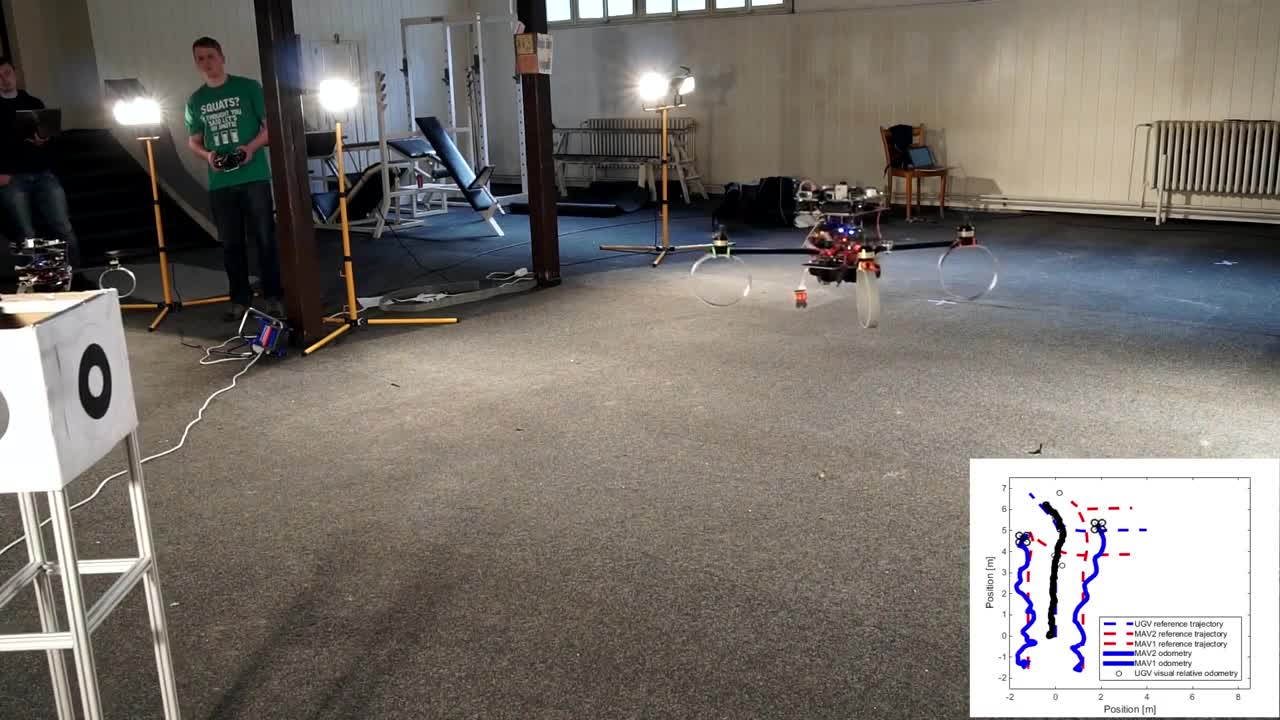
\includegraphics[width=0.7\textwidth]{fig/photos/mmar_vojta_thumbnail.jpg}
%      }{videos/mmar_vojta.mp4}\\
%      Video: \url{http://youtu.be/9Bpm4J31CgE}
%    \end{center}
%  \end{block}}

%\end{frame}

%\begin{frame}
%  \frametitle{UAV Experimentation in MRS --- 2012--2015}

%  \begin{itemize}
%    \item Custom and purpose-built hardware
%    \item Embedded software
%    {\color{red} \item not scalable! bottlenecks everywhere
%    \item embedded programming was \emph{cumbersome}
%    \item simulating was difficult (custom-built hardware did not help)
%    \item system maintenance was not flexible
%    \item low modularity
%    \item limited availability of sensors and peripheries}
%  \end{itemize}

%  \begin{block}{Publications}
%    \cite{saska2013adhoc}, \cite{chudoba2014localization}, \cite{baca2016embedded}, \cite{saska2017documentation}, \cite{chudoba2016exploration}, \cite{saska2016formations}, \cite{spurny2016complex}, \cite{saska2017system}
%  \end{block}

%\end{frame}

%%%}

%%{ Sim-to-real

\begin{frame}
\frametitle{Simulation-to-reality gap}

  \only<1>{
    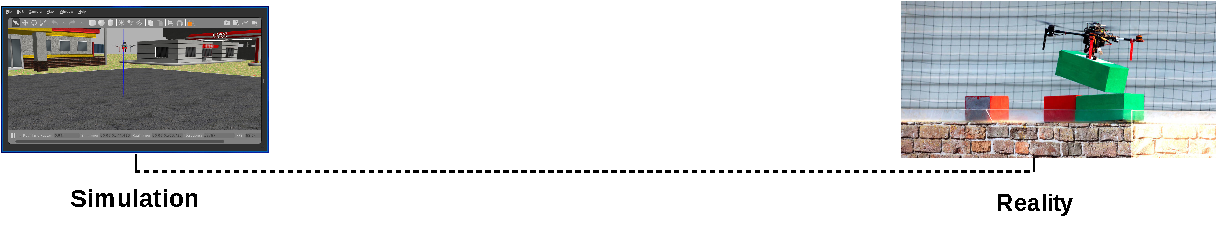
\includegraphics[width=1.0\textwidth]{./fig/sim_to_real/sim_to_real_1.pdf}
  }

  \only<2>{
    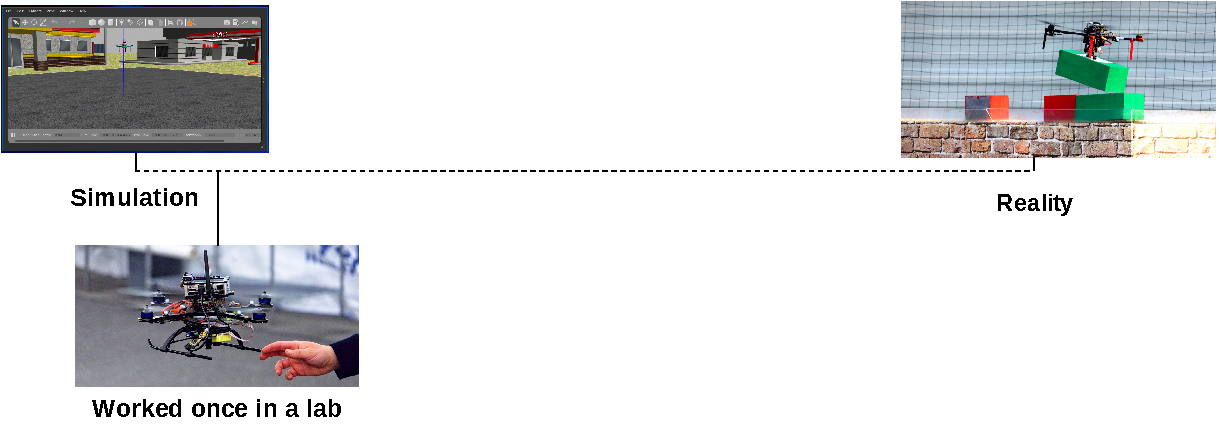
\includegraphics[width=1.0\textwidth]{./fig/sim_to_real/sim_to_real_2.pdf}
  }

  \only<3>{
    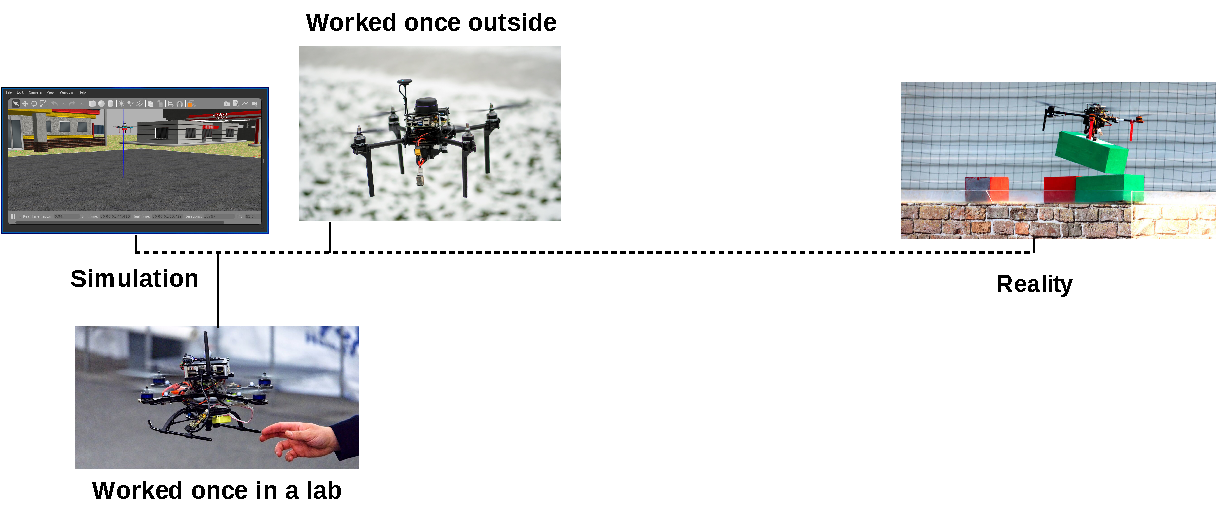
\includegraphics[width=1.0\textwidth]{./fig/sim_to_real/sim_to_real_3.pdf}
  }

  \only<4>{
    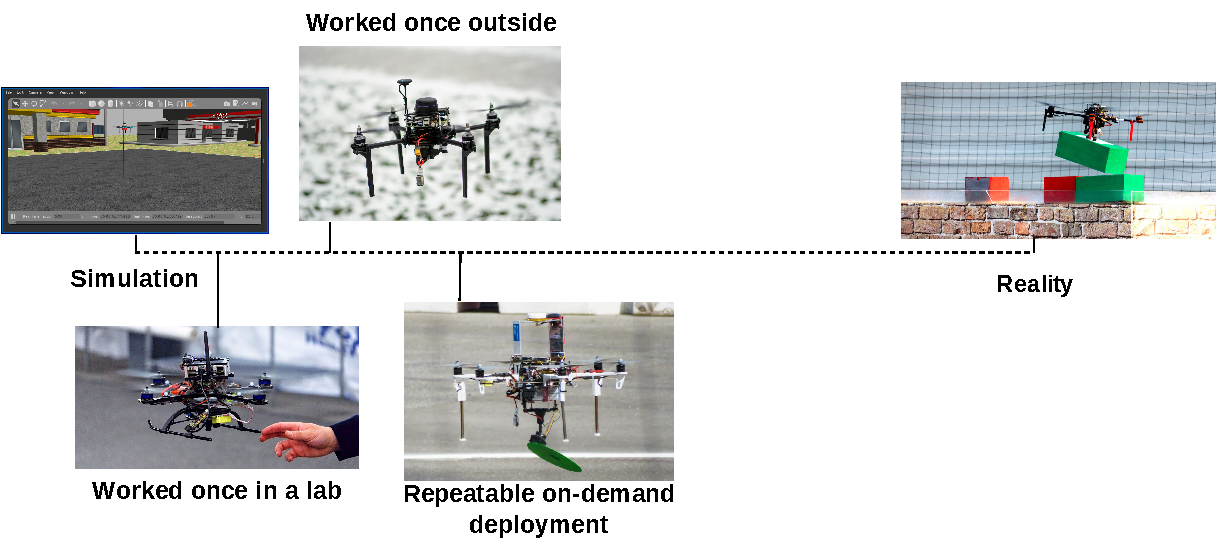
\includegraphics[width=1.0\textwidth]{./fig/sim_to_real/sim_to_real_4.pdf}
  }

  \only<5>{
    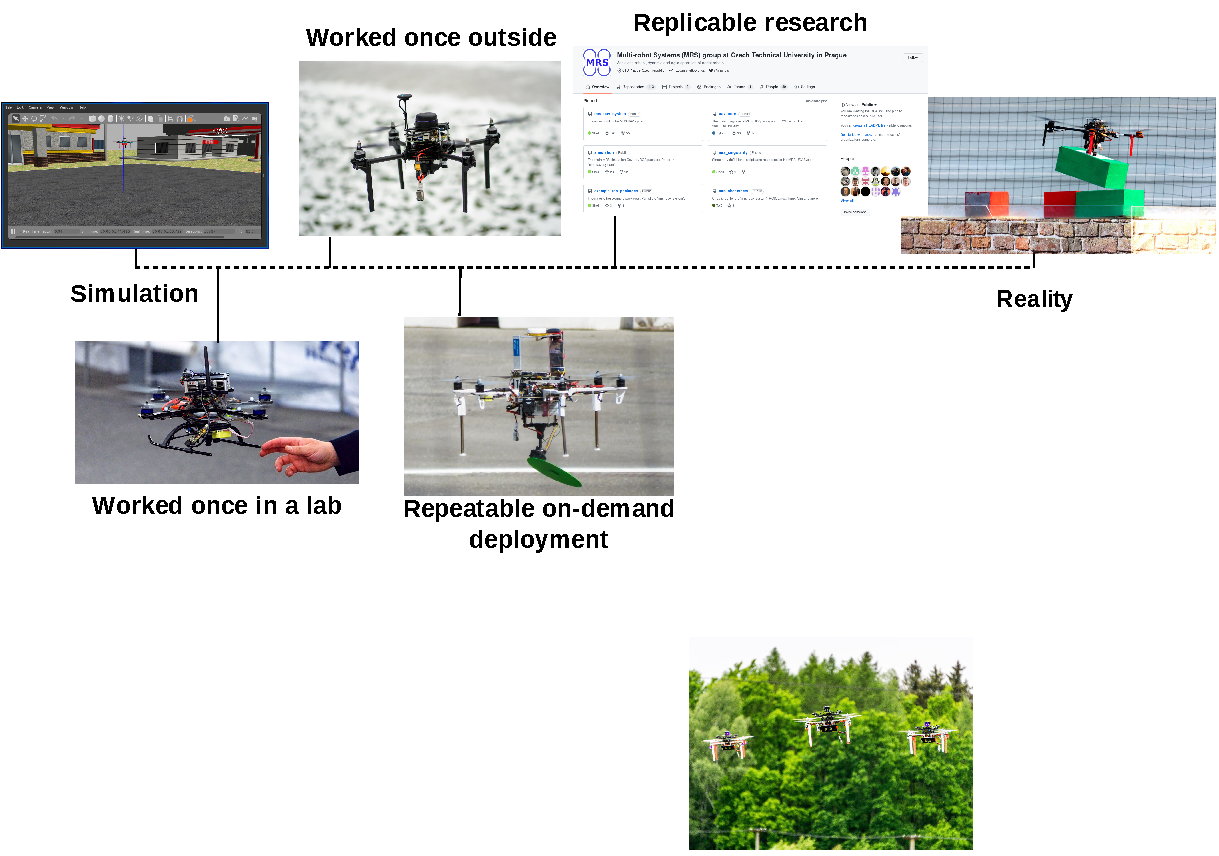
\includegraphics[width=1.0\textwidth]{./fig/sim_to_real/sim_to_real_5.pdf}
  }

  \only<6>{
    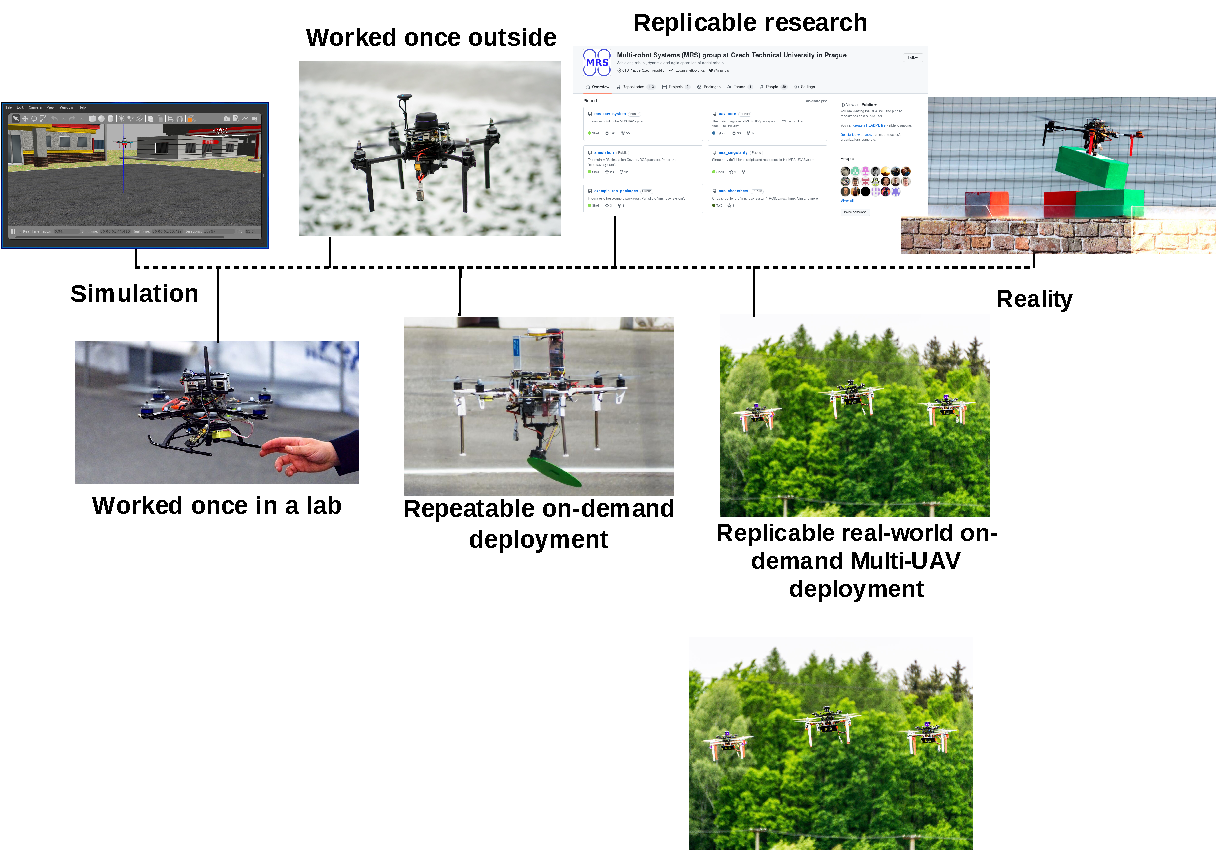
\includegraphics[width=1.0\textwidth]{./fig/sim_to_real/sim_to_real_6.pdf}
  }

\end{frame}

%%}

%%{ Research drone hardware diagram

\begin{frame}
  \frametitle{Typical research flying robot configuration}

  \begin{block}{A typical pipeline structure revolves around a Linux computer}
    \begin{figure}
      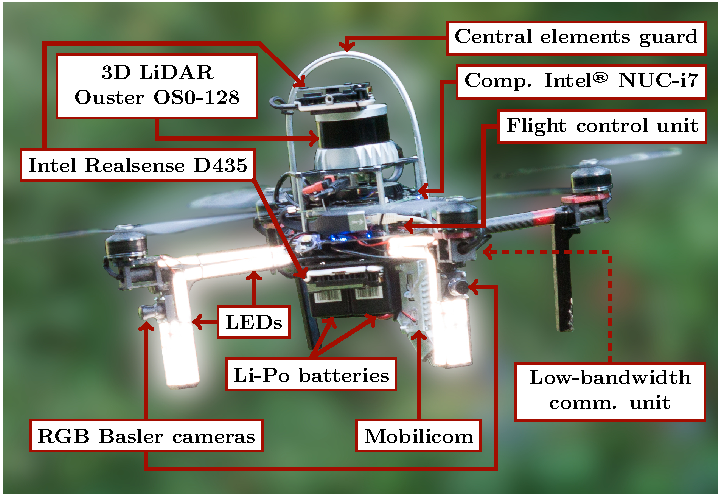
\includegraphics[width=0.6\textwidth]{fig/x500_labeled.pdf}
    \end{figure}
  \end{block}

\end{frame}

\begin{frame}
  \frametitle{Research drone (flying robot) hardware diagram}

\begin{center}
  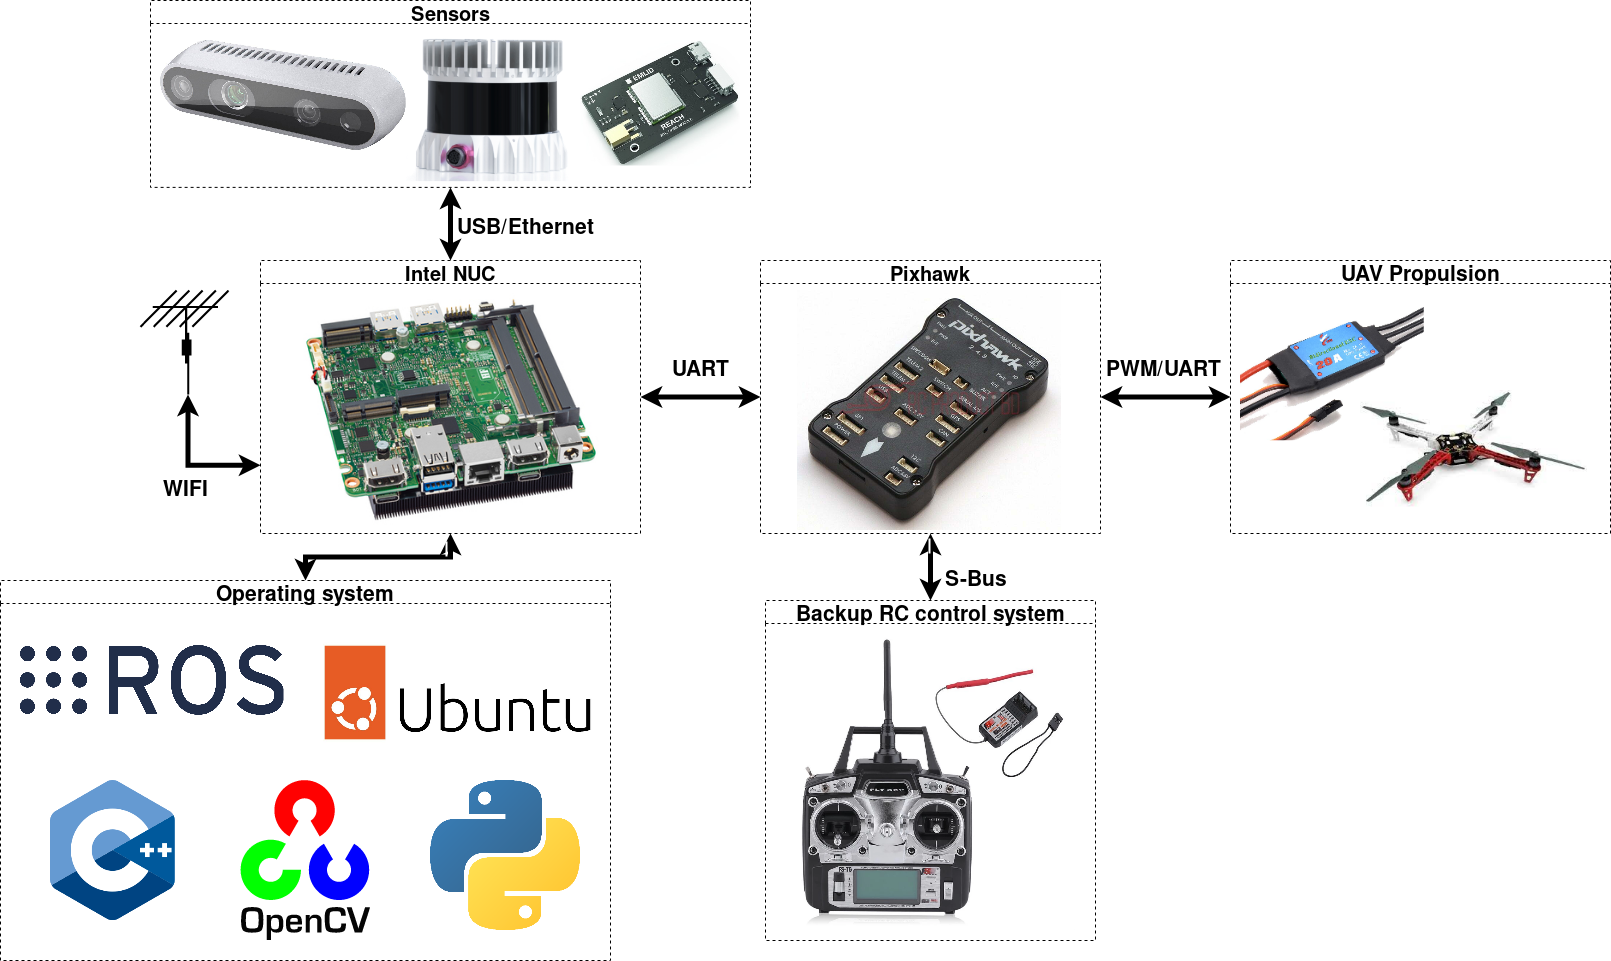
\includegraphics[width=0.8\textwidth]{./fig/new_diagram.png}
\end{center}

\end{frame}

%%}

%% | ------------ Control pipeline - implementation ----------- |

%\section{UAV Control pipeline}
%\subsection{Control -- math point of view}

%%%{ UAV control pipepline

%\begin{frame}
%  \frametitle{Control system point of view}

%  \begin{figure}
%    \begin{adjustbox}{max totalsize={1.0\textwidth}{.85\textheight}, center}
%      \pgfdeclarelayer{foreground}
\pgfsetlayers{background,main,foreground}

\tikzset{radiation/.style={{decorate,decoration={expanding waves,angle=90,segment length=4pt}}}}

\begin{tikzpicture}[->,>=stealth', node distance=3.0cm,scale=1.0, every node/.style={scale=1.0}]

  %%{ nodes

  \node[state, shift = {(0.0, 0.0)}] (navigation) {
      \begin{tabular}{c}
        \footnotesize Mission \&\\
        \footnotesize navigation
      \end{tabular}
    };

  % \node[state, left of = navigation, shift = {(0.5, 0.0)}] (nimbro) {
  %     \begin{tabular}{c}
  %       \footnotesize Nimbro \\
  %       \footnotesize Network
  %     \end{tabular}
  %   };

  \node[state, right of = navigation, shift = {(0.7, 0)}] (tracker) {
      \begin{tabular}{c}
        \footnotesize Reference \\
        \footnotesize tracker
      \end{tabular}
    };

  \node[state, right of = tracker, shift = {(0.1, 0)}] (controller) {
      \begin{tabular}{c}
        \footnotesize Reference \\
        \footnotesize controller
      \end{tabular}
    };

  \node[state, right of = controller, shift = {(0.8, -0)}] (attitude) {
      \begin{tabular}{c}
        \footnotesize Attitude rate\\
        \footnotesize controller
      \end{tabular}
    };

  \node[state, right of = attitude, shift = {(0.7, -0)}] (actuators) {
      \begin{tabular}{c}
        \footnotesize UAV \\
        \footnotesize actuators
      \end{tabular}
    };

  \node[state, right of = actuators, shift = {(-1.0, -0)}] (sensors) {
      \begin{tabular}{c}
        \footnotesize Onboard \\
        \footnotesize sensors
      \end{tabular}
    };

  \node[state, below of = attitude, shift = {(0, 1.0)}] (estimator) {
      \begin{tabular}{c}
        \footnotesize State \\
        \footnotesize estimator
      \end{tabular}
    };

  %%}

  %%{ paths

  \path[->] ($(navigation.east) + (0.0, 0)$) edge [] node[above, midway, shift = {(0.0, 0.05)}] {
      \begin{tabular}{c}
        \footnotesize desired reference\\
        \footnotesize $\mathbf{r}_d, \eta_d$\\
        \footnotesize \textit{on demand}
    \end{tabular}} ($(tracker.west) + (0.0, 0.00)$);

  % \path[->] ($(nimbro.east) + (0.0, 0)$) edge [] node[above, midway, shift = {(0.0, 0.05)}] {
  %     \begin{tabular}{c}
  %   \end{tabular}} ($(navigation.west) + (0.0, 0.00)$);

  \path[->] ($(tracker.east) + (0.0, 0)$) edge [] node[above, midway, shift = {(0.0, 0.05)}] {
      \begin{tabular}{c}
        \footnotesize full-state reference\\
        \footnotesize $\bm{\chi}_d$\\
        \footnotesize \SI{100}{\hertz}
    \end{tabular}} ($(controller.west) + (0.0, 0.00)$);

  \path[->] ($(tracker.south |- estimator.west) + (0.0, 0.0)$) edge [dotted] node[left, midway, shift = {(0.2, 0.00)}] {
      \begin{tabular}{r}
        \scriptsize initialization\\[-0.5em]
        \scriptsize only
    \end{tabular}} ($(tracker.south) + (0.0, 0.00)$);

  \path[->] ($(controller.east) + (0.0, 0)$) edge [] node[above, midway, shift = {(-0.2, 0.05)}] {
      \begin{tabular}{c}
        \footnotesize $\bm{\omega}_d$\\
        \footnotesize $T_d$ \\
        \footnotesize \SI{100}{\hertz}
    \end{tabular}} ($(attitude.west) + (0.0, 0.00)$);

  \draw[-] ($(controller.south)+(0.25,0)$) -- ($(controller.south |- estimator.west) + (0.25, 0.25)$) edge [->] node[above, near start, shift = {(-0.2, 0.05)}] {
      \begin{tabular}{c}
        \footnotesize $\mathbf{a}_d$
    \end{tabular}} ($(estimator.west) + (0, 0.25)$);

  \path[->] ($(attitude.east) + (0.0, 0)$) edge [] node[above, midway, shift = {(0.1, 0.05)}] {
      \begin{tabular}{c}
        \footnotesize $\bm{\tau}_d$ \\
        \footnotesize $\approx$\SI{1}{\kilo\hertz}
    \end{tabular}} ($(actuators.west) + (0.0, 0.00)$);

  \path[-] ($(estimator.west)+(0, 0)$) edge [] node[above, near start, shift = {(-1.0, 0.0)}] {
      \begin{tabular}{c}
        \footnotesize $\mathbf{x}$, $\mathbf{R}$, $\bm{\omega}$\\
        \footnotesize \SI{100}{\hertz}
    \end{tabular}} ($(navigation.south |- estimator.west)$) -- ($(navigation.south |- estimator.west)$) edge [->,] ($(navigation.south)+(0, 0)$);

  % \path[-] ($(estimator.west)+(0, 0)$) edge [] node[above, near start, shift = {(-1.0, 0.0)}] {
  %     \begin{tabular}{c}
  %   \end{tabular}} ($(nimbro.south |- estimator.west)$) -- ($(nimbro.south |- estimator.west)$) edge [->,] ($(nimbro.south)+(0, 0)$);

  \path[->] ($(controller.south |- estimator.west)+(0, 0)$) edge [] ($(controller.south)$);

  \path[->] ($(attitude.south) + (0.0, -0.1)$) edge [] node[right, midway, shift = {(0.0, 0.00)}] {
      \begin{tabular}{c}
        \footnotesize $\mathbf{R}$, $\bm{\omega}$
    \end{tabular}} ($(estimator.north) + (0.0, 0.00)$);

  \path[-] ($(sensors.south)+(0, 0)$) edge [] ($(sensors.south |- estimator.east)$) -- ($(sensors.south |- estimator.east)$) edge [->,] node[above, near start, shift = {(-0.35, -0.1)}] {
      \begin{tabular}{c}
        \footnotesize onboard sensor data
    \end{tabular}}($(estimator.east)$);

  %%}

    % \draw[-, radiation, decoration={angle=45}] ($(nimbro.west) + (0.0, -0.0)$) -- +(0:-0.5);

  %%{ backgrounds

  \begin{pgfonlayer}{background}
    \path (attitude.west |- attitude.north)+(-0.45,0.8) node (a) {};
    \path (sensors.south -| sensors.east)+(+0.25,-0.20) node (b) {};
    \path[fill=gray!3,rounded corners, draw=black!70, densely dotted]
      (a) rectangle (b);
  \end{pgfonlayer}
  \node [rectangle, above of=actuators, shift={(-0.6,0.55)}, node distance=1.7em] (autopilot) {\footnotesize UAV plant};

  \begin{pgfonlayer}{background}
    \path (attitude.west |- attitude.north)+(-0.25,0.47) node (a) {};
    \path (attitude.south -| attitude.east)+(+0.25,-0.10) node (b) {};
    \path[fill=gray!3,rounded corners, draw=black!70, densely dotted]
      (a) rectangle (b);
  \end{pgfonlayer}
  \node [rectangle, above of=attitude, shift={(0,0.2)}, node distance=1.7em] (autopilot) {\footnotesize Embedded autopilot};

  %%}

\end{tikzpicture}

%    \end{adjustbox}
%  \end{figure}

%  \fullciteinbox{baca2021mrs}{}

%\end{frame}

%%}

%\subsection{Control -- implementation point of view}

%%%{ From theory to practical experiments

%%%{ Linear Kalman filter

%\begin{frame}
%  \frametitle{From theory to practical experiments}

%  \begin{columns}[c]

%    \onslide<1->{\column{0.48\textwidth} % Left column and width
%    \begin{block}{Linear Kalman Filter $\approx$ 10 lines}
%      \begin{adjustbox}{max totalsize={1.0\textwidth}{.85\textheight}, center}
%        \begin{tikzpicture}[->,>=stealth']

% Position of PREDICTION
% Use previously defined 'state' as layout (see above)
% use tabular for content to get columns/rows
  % parbox to limit width of the listing
\node[state] (PREDICTION)
{
  \begin{tabular}{c}
  Prediction phase\\
    \begin{tabular}{rcl}
  $\hat{\textbf{x}}_{[t]}$ & $\leftarrow$ & $\textbf{A}\hat{\textbf{x}}_{[t-1]} + \textbf{B}\textbf{u}_{[t-1]}$ \\
    $\hat{\boldsymbol{\Sigma}}_{[t]}$ & $\leftarrow$ & $\textbf{A}\hat{\boldsymbol{\Sigma}}_{[t-1]}\textbf{A}^{T} + \textbf{R}$
    \end{tabular}
  \end{tabular}
};

  % State: CORRECTION with different content
\node[state,    	% layout (defined above)
  below of=PREDICTION, 	% Position is to the right of PREDICTION
  node distance=3.5cm, 	% distance to PREDICTION
  anchor=center] (CORRECTION) 	% posistion relative to the center of the 'box'
{%
  \begin{tabular}{c}
  Correction phase\\
    \begin{tabular}{rcl}
  $\textbf{K}_{[t]}$ & $\leftarrow$ & $\hat{\boldsymbol{\Sigma}}_{[t]}\textbf{W}^{T}\left(\textbf{W}\hat{\boldsymbol{\Sigma}}_{[t]}\textbf{W}^{T} + \textbf{M}\right)^{-1}$ \\
    $\hat{\textbf{x}}_{[t]}$ & $\leftarrow$ & $\hat{\textbf{x}}_{[t]} + \textbf{K}_{[t]}\left(\textbf{z}_{[t]} - \textbf{W}\hat{\textbf{x}}_{[t]}\right)$ \\
    $\hat{\boldsymbol{\Sigma}}_{[t]}$ & $\leftarrow$ & $\left(\mathbf{I} - \textbf{K}_{[t]}\textbf{W}\right)\hat{\boldsymbol{\Sigma}}_{[t]}$ \\
    \end{tabular}
  \end{tabular}
};

\node[nothing,    	% layout (defined above)
  left of=PREDICTION, 	% Position is to the right of QUERY
  node distance=5cm, 	% distance to QUERY
  anchor=center] (PRED_IN) 	% posistion relative to the center of the 'box'
{};

\node[nothing,    	% layout (defined above)
  left of=CORRECTION, 	% Position is to the right of QUERY
  node distance=6cm, 	% distance to QUERY
  anchor=center] (CORR_IN) 	% posistion relative to the center of the 'box'
{};

% draw the paths and and print some Text below/above the graph
\path (PREDICTION) 	edge[bend left=30]  node[anchor=west]
{
  $\hat{\textbf{x}}_{[t]}$, $\hat{\boldsymbol{\Sigma}}_{[t]}$
} (CORRECTION)
(CORRECTION) 	edge[bend left=30]  node[anchor=east]
{
  \begin{tabular}{c}
  $\hat{\textbf{x}}_{[t]}$, $\hat{\boldsymbol{\Sigma}}_{[t]}$ \\
    $t \leftarrow t + 1$
    \end{tabular}
} (PREDICTION)

(PRED_IN) edge[] node[anchor=south] {Input} node[anchor=north] {\textbf{u}} (PREDICTION)

  (CORR_IN) edge[] node[anchor=south] {Measure} node[anchor=north] {$\textbf{z}, \textbf{M}, \textbf{W}$} (CORRECTION);

  \end{tikzpicture}

%      \end{adjustbox}
%    \end{block}}

%    \onslide<2>{\column{0.48\textwidth} % Right column and width
%    \begin{block}{Linear Kalman Filter in practice}
%      \begin{itemize}
%        \item tens of lines in Matlab
%        \item $\ge$ 1000 lines of \texttt{C++} code
%        \item Real-world fusion \& estimation\\
%          $\ge$ 20 000 lines of \texttt{C++} code
%      \end{itemize}
%    \end{block}}

%  \end{columns}

%\end{frame}

%%%}

%%%{ Control

%\begin{frame}
%  \frametitle{From theory to practical experiments}

%  \begin{columns}[c]

%    \column{0.60\textwidth} % Left column and width
%    \onslide<1->{\vspace{-1em}
%\begin{block}{Geometric tracking controller $\approx$ 10 lines}
%\vspace{-1em}
%\tiny\begin{align}
%\mathbf{f}_d &= \minus m_e\mathbf{k}_p\circ \mathbf{e}_p \minus m_e\mathbf{k}_v\circ \mathbf{e}_v \plus m_e\ddot{\mathbf{r}}_d \minus m_eg\mathbf{\hat{e}}_3 \minus \mathbf{d}_w\circ \left[\begin{smallmatrix}
%1\\
%1\\
%0
%\end{smallmatrix}\right] \minus \mathbf{d}_b\circ \left[\begin{smallmatrix}
%1\\
%1\\
%0
%\end{smallmatrix}\right],\nonumber\\
%\mathbf{e}_R &= \frac{1}{2}\left(\mathbf{R}_d^\intercal\mathbf{R} - \mathbf{R}^\intercal\mathbf{R}_d\right),\nonumber\\
%\bm{\omega}_d &= \minus \mathbf{k}_R\circ \mathbf{e}_R \plus \bm{\omega}_j \minus \bm{\omega}_c,\nonumber
%\end{align}
%\vspace{-1em}
%\end{block}}

%\onslide<2->{
%\vspace{-0.5em}
%\begin{block}{MPC controller $\approx$ 100 lines}
%\vspace{-1em}
%\scriptsize{
%\begin{align*}
%  & \min_{\mathbf{u}_{[1:n]}}\nonumber
%  & \frac{1}{2}\sum_{i=1}^{n-1}\left(\mathbf{e}^\intercal_{[i]}\mathbf{Q}\mathbf{e}_{[i]}\right) + \mathbf{e}^\intercal_{[n]}\mathbf{S}\mathbf{e}_{[n]}
%\end{align*}\begin{align*}
%  \text{s.t.}~ \mathbf{x}_{m[i]} &= \mathbf{A}_m\mathbf{x}_{m[i-1]} \plus \mathbf{B}_m\mathbf{u}_{[i]}, &\forall i &\in \{1, \hdots, n\}\nonumber\\
%  \mathbf{x}_{m[i]} &\leq \mathbf{x}_{\mathrm{max}}, &\forall i &\in \{1, \hdots, n\}\nonumber\\
%  \mathbf{x}_{m[i]} &\geq \minus \mathbf{x}_{\mathrm{max}}, &\forall i &\in \{1, \hdots, n\}\nonumber \\
%  \mathbf{u}_{[i]} \minus \mathbf{u}_{[i\minus 1]} &\leq \dot{\mathbf{u}}_{\mathrm{max}} \Delta t, &\forall i &\in \{2, \hdots, n\}\nonumber\\
%  \mathbf{u}_{[i]} \minus \mathbf{u}_{[i\minus 1]} &\geq \minus \dot{\mathbf{u}}_{\mathrm{max}} \Delta t, &\forall i &\in \{2, \hdots, n\}\nonumber
%\end{align*}
%}
%\vspace{-1em}
%\end{block}}

%\column{0.38\textwidth} % Right column and width

%\onslide<3>{\begin{block}{UAV Control in practice}
%\begin{itemize}
%\item $\ge$ 10 000 lines of \texttt{C++} code
%\end{itemize}
%\end{block}}

%\end{columns}

%\end{frame}

%%%}

%%%{ From theory to practical experiments

%\begin{frame}
%  \frametitle{From theory to practical experiments}

%  \begin{columns}[c]

%    \column{0.70\textwidth} % Left column and width
%    \begin{block}{What needs to be solved outside of Matlab's sandbox?}
%      \begin{itemize}
%        \item UAV crashes are expensive, so don't crash
%        \item Software runtime errors cause UAV crashes
%        \item control references might not be feasible
%        \item sensors can get disconnected during the flight
%        \item takeoff and landing: \textbf{the most tricky part of the flight}
%        \item mass (and the model) can change during the flight
%        \item controllers can be poorly tuned... handle instabilities
%        \item acceleration and speed depend on the available sensors
%        \item people are fallible, don't let them crash the drones
%        \item not all states of UAV are allowed, even though controllers can reach them (upside down)
%      \end{itemize}
%    \end{block}

%    \column{0.28\textwidth} % Right column and width
%    \begin{block}{The failsafe core}
%      \texttt{if (goingToCrash())}\\
%      \texttt{~~~~dont();}
%    \end{block}

%  \end{columns}

%\end{frame}

%%%}

%\begin{frame}
%\frametitle{Pushing the chances --- 14 UAVs in a swarm}

%  \begin{center}
%    \mymovie[autostart,loop]{
%      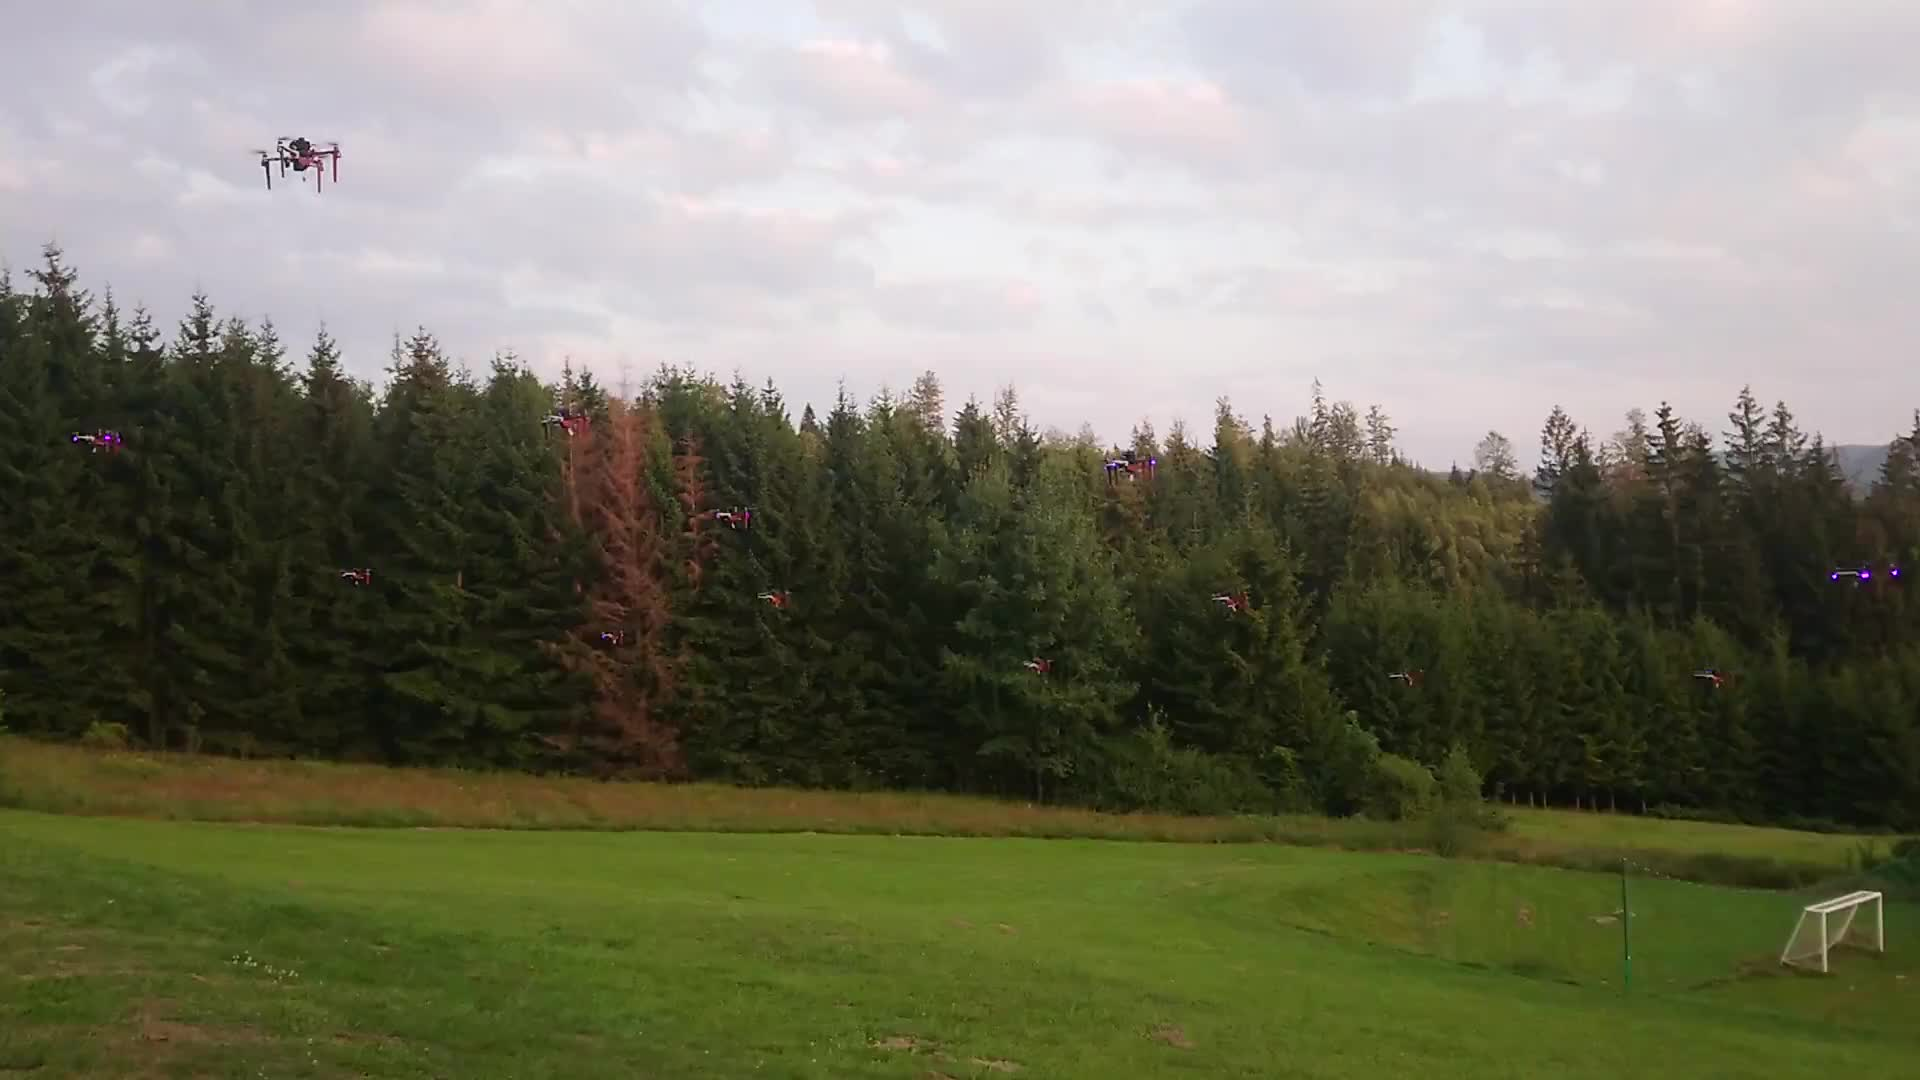
\includegraphics[width=0.9\textwidth]{./fig/swarm_14uavs_field_thumbnail.jpg}
%    }{./videos/swarm_14uavs_field.mp4}\\
%  \end{center}

%\end{frame}

%\begin{frame}
%\frametitle{Pushing the chances too much}

%\begin{center}
%  \mymovie[autostart,loop,start=5]{
%    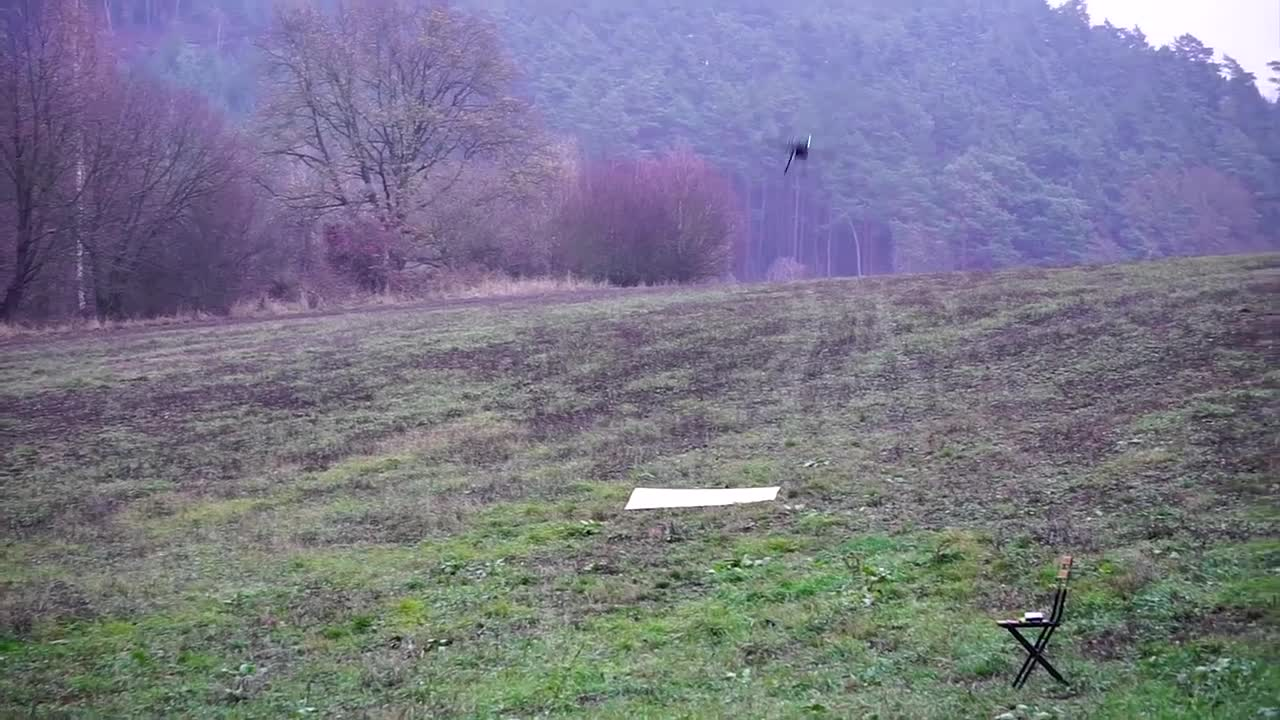
\includegraphics[width=0.75\textwidth]{./fig/crashes_thumbnail.jpg}
%  }{./videos/crashes.mp4}\\
%  Video: \url{https://youtu.be/dT7b1j5Ij1I?t=148}
%\end{center}

%\end{frame}

%%%}

%% | --------------------- MRS UAV System --------------------- |

%%{ System diagram

\begin{frame}

\frametitle{The MRS UAV System - control system PoV}

  \begin{block}{MRS UAV System block diagram}
    \begin{figure}
      \begin{adjustbox}{max totalsize={1.0\textwidth}{.65\textheight}, center}
        \only<1>{\pgfdeclarelayer{foreground}
\pgfsetlayers{background,main,foreground}

\tikzset{radiation/.style={{decorate,decoration={expanding waves,angle=90,segment length=4pt}}}}

\begin{tikzpicture}[->,>=stealth', node distance=3.0cm,scale=1.0, every node/.style={scale=1.0}]

  %%{ nodes

  \node[state, shift = {(0.0, 0.0)}] (navigation) {
      \begin{tabular}{c}
        \footnotesize Mission \&\\
        \footnotesize navigation
      \end{tabular}
    };

  % \node[state, left of = navigation, shift = {(0.5, 0.0)}] (nimbro) {
  %     \begin{tabular}{c}
  %       \footnotesize Nimbro \\
  %       \footnotesize Network
  %     \end{tabular}
  %   };

  \node[state, right of = navigation, shift = {(0.7, 0)}] (tracker) {
      \begin{tabular}{c}
        \footnotesize Reference \\
        \footnotesize tracker
      \end{tabular}
    };

  \node[state, right of = tracker, shift = {(0.1, 0)}] (controller) {
      \begin{tabular}{c}
        \footnotesize Reference \\
        \footnotesize controller
      \end{tabular}
    };

  \node[state, right of = controller, shift = {(0.8, -0)}] (attitude) {
      \begin{tabular}{c}
        \footnotesize Attitude rate\\
        \footnotesize controller
      \end{tabular}
    };

  \node[state, right of = attitude, shift = {(0.7, -0)}] (actuators) {
      \begin{tabular}{c}
        \footnotesize UAV \\
        \footnotesize actuators
      \end{tabular}
    };

  \node[state, right of = actuators, shift = {(-1.0, -0)}] (sensors) {
      \begin{tabular}{c}
        \footnotesize Onboard \\
        \footnotesize sensors
      \end{tabular}
    };

  \node[state, below of = attitude, shift = {(0, 1.0)}] (estimator) {
      \begin{tabular}{c}
        \footnotesize State \\
        \footnotesize estimator
      \end{tabular}
    };

  %%}

  %%{ paths

  \path[->] ($(navigation.east) + (0.0, 0)$) edge [] node[above, midway, shift = {(0.0, 0.05)}] {
      \begin{tabular}{c}
        \footnotesize desired reference\\
        \footnotesize $\mathbf{r}_d, \eta_d$\\
        \footnotesize \textit{on demand}
    \end{tabular}} ($(tracker.west) + (0.0, 0.00)$);

  % \path[->] ($(nimbro.east) + (0.0, 0)$) edge [] node[above, midway, shift = {(0.0, 0.05)}] {
  %     \begin{tabular}{c}
  %   \end{tabular}} ($(navigation.west) + (0.0, 0.00)$);

  \path[->] ($(tracker.east) + (0.0, 0)$) edge [] node[above, midway, shift = {(0.0, 0.05)}] {
      \begin{tabular}{c}
        \footnotesize full-state reference\\
        \footnotesize $\bm{\chi}_d$\\
        \footnotesize \SI{100}{\hertz}
    \end{tabular}} ($(controller.west) + (0.0, 0.00)$);

  \path[->] ($(tracker.south |- estimator.west) + (0.0, 0.0)$) edge [dotted] node[left, midway, shift = {(0.2, 0.00)}] {
      \begin{tabular}{r}
        \scriptsize initialization\\[-0.5em]
        \scriptsize only
    \end{tabular}} ($(tracker.south) + (0.0, 0.00)$);

  \path[->] ($(controller.east) + (0.0, 0)$) edge [] node[above, midway, shift = {(-0.2, 0.05)}] {
      \begin{tabular}{c}
        \footnotesize $\bm{\omega}_d$\\
        \footnotesize $T_d$ \\
        \footnotesize \SI{100}{\hertz}
    \end{tabular}} ($(attitude.west) + (0.0, 0.00)$);

  \draw[-] ($(controller.south)+(0.25,0)$) -- ($(controller.south |- estimator.west) + (0.25, 0.25)$) edge [->] node[above, near start, shift = {(-0.2, 0.05)}] {
      \begin{tabular}{c}
        \footnotesize $\mathbf{a}_d$
    \end{tabular}} ($(estimator.west) + (0, 0.25)$);

  \path[->] ($(attitude.east) + (0.0, 0)$) edge [] node[above, midway, shift = {(0.1, 0.05)}] {
      \begin{tabular}{c}
        \footnotesize $\bm{\tau}_d$ \\
        \footnotesize $\approx$\SI{1}{\kilo\hertz}
    \end{tabular}} ($(actuators.west) + (0.0, 0.00)$);

  \path[-] ($(estimator.west)+(0, 0)$) edge [] node[above, near start, shift = {(-1.0, 0.0)}] {
      \begin{tabular}{c}
        \footnotesize $\mathbf{x}$, $\mathbf{R}$, $\bm{\omega}$\\
        \footnotesize \SI{100}{\hertz}
    \end{tabular}} ($(navigation.south |- estimator.west)$) -- ($(navigation.south |- estimator.west)$) edge [->,] ($(navigation.south)+(0, 0)$);

  % \path[-] ($(estimator.west)+(0, 0)$) edge [] node[above, near start, shift = {(-1.0, 0.0)}] {
  %     \begin{tabular}{c}
  %   \end{tabular}} ($(nimbro.south |- estimator.west)$) -- ($(nimbro.south |- estimator.west)$) edge [->,] ($(nimbro.south)+(0, 0)$);

  \path[->] ($(controller.south |- estimator.west)+(0, 0)$) edge [] ($(controller.south)$);

  \path[->] ($(attitude.south) + (0.0, -0.1)$) edge [] node[right, midway, shift = {(0.0, 0.00)}] {
      \begin{tabular}{c}
        \footnotesize $\mathbf{R}$, $\bm{\omega}$
    \end{tabular}} ($(estimator.north) + (0.0, 0.00)$);

  \path[-] ($(sensors.south)+(0, 0)$) edge [] ($(sensors.south |- estimator.east)$) -- ($(sensors.south |- estimator.east)$) edge [->,] node[above, near start, shift = {(-0.35, -0.1)}] {
      \begin{tabular}{c}
        \footnotesize onboard sensor data
    \end{tabular}}($(estimator.east)$);

  %%}

    % \draw[-, radiation, decoration={angle=45}] ($(nimbro.west) + (0.0, -0.0)$) -- +(0:-0.5);

  %%{ backgrounds

  \begin{pgfonlayer}{background}
    \path (attitude.west |- attitude.north)+(-0.45,0.8) node (a) {};
    \path (sensors.south -| sensors.east)+(+0.25,-0.20) node (b) {};
    \path[fill=gray!3,rounded corners, draw=black!70, densely dotted]
      (a) rectangle (b);
  \end{pgfonlayer}
  \node [rectangle, above of=actuators, shift={(-0.6,0.55)}, node distance=1.7em] (autopilot) {\footnotesize UAV plant};

  \begin{pgfonlayer}{background}
    \path (attitude.west |- attitude.north)+(-0.25,0.47) node (a) {};
    \path (attitude.south -| attitude.east)+(+0.25,-0.10) node (b) {};
    \path[fill=gray!3,rounded corners, draw=black!70, densely dotted]
      (a) rectangle (b);
  \end{pgfonlayer}
  \node [rectangle, above of=attitude, shift={(0,0.2)}, node distance=1.7em] (autopilot) {\footnotesize Embedded autopilot};

  %%}

\end{tikzpicture}
}
        \only<2>{\pgfdeclarelayer{foreground}
\pgfsetlayers{background,main,foreground}

\tikzset{radiation/.style={{decorate,decoration={expanding waves,angle=90,segment length=4pt}}}}

\begin{tikzpicture}[->,>=stealth', node distance=3.0cm,scale=1.0, every node/.style={scale=1.0}]

  %%{ nodes

  \node[state, shift = {(0.0, 0.0)}] (navigation) {
      \begin{tabular}{c}
        \footnotesize Trajectory \&\\
        \footnotesize generation
      \end{tabular}
    };

  % \node[state, left of = navigation, shift = {(0.5, 0.0)}] (nimbro) {
  %     \begin{tabular}{c}
  %       \footnotesize Nimbro \\
  %       \footnotesize Network
  %     \end{tabular}
  %   };

  \node[state, right of = navigation, shift = {(0.7, 0)}] (tracker) {
      \begin{tabular}{c}
        \footnotesize Reference \\
        \footnotesize tracker
      \end{tabular}
    };

  \node[state_focus, right of = tracker, shift = {(0.1, 0)}] (controller) {
      \begin{tabular}{c}
        \footnotesize Reference \\
        \footnotesize controller
      \end{tabular}
    };

  \node[state, right of = controller, shift = {(0.8, -0)}] (attitude) {
      \begin{tabular}{c}
        \footnotesize Attitude rate\\
        \footnotesize controller
      \end{tabular}
    };

  \node[smallstate, below of = attitude, shift = {(-0.6, 2.05)}] (imu) {
      \footnotesize IMU
    };

  \node[state, right of = attitude, shift = {(0.7, -0)}] (actuators) {
      \begin{tabular}{c}
        \footnotesize UAV \\
        \footnotesize actuators
      \end{tabular}
    };

  \node[state, right of = actuators, shift = {(-0.8, -0)}] (sensors) {
      \begin{tabular}{c}
        \footnotesize Onboard \\
        \footnotesize sensors
      \end{tabular}
    };

  \node[state, below of = attitude, shift = {(0, 0.9)}] (estimator) {
      \begin{tabular}{c}
        \footnotesize State \\
        \footnotesize estimator
      \end{tabular}
    };

  \node[state, right of = estimator, shift = {(0.8, 0.0)}] (localization) {
      \begin{tabular}{c}
        \footnotesize Odometry \& \\
        \footnotesize localization
      \end{tabular}
    };

  %%}

  %%{ paths

  \path[->] ($(navigation.east) + (0.0, 0)$) edge [] node[above, midway, shift = {(0.0, 0.05)}] {
      \begin{tabular}{c}
        \footnotesize desired reference\\
        \footnotesize $\mathbf{r}_d, \eta_d$\\
        \footnotesize \textit{on demand}
    \end{tabular}} ($(tracker.west) + (0.0, 0.00)$);

  % \path[->] ($(nimbro.east) + (0.0, 0)$) edge [] node[above, midway, shift = {(0.0, 0.05)}] {
  %     \begin{tabular}{c}
  %   \end{tabular}} ($(navigation.west) + (0.0, 0.00)$);

  \path[->] ($(tracker.east) + (0.0, 0)$) edge [] node[above, midway, shift = {(0.0, 0.05)}] {
      \begin{tabular}{c}
        \footnotesize full-state reference\\
        \footnotesize $\bm{\chi}_d$\\
        \footnotesize \SI{100}{\hertz}
    \end{tabular}} ($(controller.west) + (0.0, 0.00)$);

  \path[->] ($(tracker.south |- estimator.west) + (0.0, 0.0)$) edge [dotted] node[left, midway, shift = {(0.2, 0.00)}] {
      \begin{tabular}{r}
        \scriptsize initialization\\[-0.5em]
        \scriptsize only
    \end{tabular}} ($(tracker.south) + (0.0, 0.00)$);

  \path[->] ($(controller.east) + (0.0, 0)$) edge [] node[above, midway, shift = {(-0.2, 0.05)}] {
      \begin{tabular}{c}
        \footnotesize $\bm{\omega}_d$\\
        \footnotesize $T_d$ \\
        \footnotesize \SI{100}{\hertz}
    \end{tabular}} ($(attitude.west) + (0.0, 0.00)$);

  \draw[-] ($(controller.south)+(0.25,0)$) -- ($(controller.south |- estimator.west) + (0.25, 0.25)$) edge [->] node[above, near start, shift = {(-0.2, 0.05)}] {
      \begin{tabular}{c}
        \footnotesize $\mathbf{a}_d$
    \end{tabular}} ($(estimator.west) + (0, 0.25)$);

  \path[->] ($(attitude.east) + (0.0, 0)$) edge [] node[above, midway, shift = {(0.1, 0.05)}] {
      \begin{tabular}{c}
        \footnotesize $\bm{\tau}_d$ \\
        \footnotesize $\approx$\SI{1}{\kilo\hertz}
    \end{tabular}} ($(actuators.west) + (0.0, 0.00)$);

  \path[-] ($(estimator.west)+(0, 0)$) edge [] node[above, near start, shift = {(-1.0, 0.0)}] {
      \begin{tabular}{c}
        \footnotesize $\mathbf{x}$, $\mathbf{R}$, $\bm{\omega}$\\
        \footnotesize \SI{100}{\hertz}
    \end{tabular}} ($(navigation.south |- estimator.west)$) -- ($(navigation.south |- estimator.west)$) edge [->,] ($(navigation.south)+(0, 0)$);

  % \path[-] ($(estimator.west)+(0, 0)$) edge [] node[above, near start, shift = {(-1.0, 0.0)}] {
  %     \begin{tabular}{c}
  %   \end{tabular}} ($(nimbro.south |- estimator.west)$) -- ($(nimbro.south |- estimator.west)$) edge [->,] ($(nimbro.south)+(0, 0)$);

  \path[->] ($(controller.south |- estimator.west)+(0, 0)$) edge [] ($(controller.south)$);

  \draw[-] ($(imu.east) + (0.0, 0.0)$) -- ($(estimator.north |- imu.east) + (0.3, 0)$) edge [->] node[right, midway, shift = {(-0.2, 0.3)}] {
      \begin{tabular}{c}
        \footnotesize $\mathbf{R}$, $\bm{\omega}$
    \end{tabular}} ($(estimator.north) + (0.3, 0.0)$);

  \draw[-] ($(sensors.south)+(0, 0)$) -- ($(sensors.south |- localization.east)$) edge [->] ($(localization.east)$);
  \draw[-] ($(sensors.south)+(0.1, 0)$) -- ($(sensors.south |- localization.east) + (0.1, -0.1)$) edge [->] ($(localization.east) + (0.0, -0.1)$);
  \draw[-] ($(sensors.south)+(-0.1, 0)$) -- ($(sensors.south |- localization.east) + (-0.1, 0.1)$) edge [->]  ($(localization.east) + (0.0, 0.1)$);

  \draw[->] ($(localization.west)+(0, 0)$) -- ($(estimator.east)$);
  \draw[->] ($(localization.west)+(0, 0.1)$) -- ($(estimator.east) + (0, 0.1)$);
  \draw[->] ($(localization.west)+(0, -0.1)$) -- ($(estimator.east) + (0, -0.1)$);

  %%}

    % \draw[-, radiation, decoration={angle=45}] ($(nimbro.west) + (0.0, -0.0)$) -- +(0:-0.5);

  %%{ backgrounds

  \begin{pgfonlayer}{background}
    \path (attitude.west |- attitude.north)+(-0.45,0.8) node (a) {};
    \path (imu.south -| sensors.east)+(+0.25,-0.20) node (b) {};
    \path[rounded corners, draw=black!70, densely dotted]
      (a) rectangle (b);
  \end{pgfonlayer}
  \node [rectangle, above of=actuators, shift={(-0.6,0.55)}, node distance=1.7em] (autopilot) {\footnotesize UAV plant};

  \begin{pgfonlayer}{background}
    \path (attitude.west |- attitude.north)+(-0.25,0.47) node (a) {};
    \path (imu.south -| attitude.east)+(+0.25,-0.10) node (b) {};
    \path[rounded corners, draw=black!70, densely dotted]
      (a) rectangle (b);
  \end{pgfonlayer}
  \node [rectangle, above of=attitude, shift={(0,0.2)}, node distance=1.7em] (autopilot) {\footnotesize Embedded autopilot};

  %%}

\end{tikzpicture}
}
      \end{adjustbox}
    \end{figure}
  \end{block}

  \fullciteinbox{baca2021mrs}{}

\end{frame}

%%}

\subsection{Reference controllers}

%%{ Reference controllers

%%{ Heading-compliant control design

\begin{frame}
\frametitle{Reference controllers --- Attitude rate}

\begin{block}{\small Heading-compliant control design}
  \small Heading $\eta = \mathrm{atan2}\left(\mathbf{\hat{b}}_1^\intercal\mathbf{\hat{e}}_2, \mathbf{\hat{b}}_1^\intercal\mathbf{\hat{e}}_1\right) = \mathrm{atan2}\left(\mathbf{h}_{(2)}, \mathbf{h}_{(1)}\right)$ as the $4^{\mathrm{th}}$ DOF (instead of \emph{yaw)}.
\end{block}

\begin{columns}[c]

\column{0.48\textwidth} % Left column and width

\begin{block}{\small \emph{SO(3)} attitude controller \cite{lee2010geometric}}
  \begin{itemize}
    \item \scriptsize Custom heading-compliant desired orientation:
  \end{itemize}

  \begin{equation}
    \scriptsize
    \mathbf{R}_d = \left[\mathbf{\hat{b}}_{1d}, \mathbf{\hat{b}}_{2d}, \mathbf{\hat{b}}_{3d}\right],
  \end{equation}

  \begin{equation}
    \scriptsize
    \mathbf{b}_{1d} = \mathbf{O}(\mathbf{P}^\intercal\mathbf{O})^{-1}\mathbf{P}^\intercal\,\mathbf{\hat{h}}_d,\ \mathbf{\hat{b}}_{1d} = \frac{\mathbf{b}_{1d}}{\|\mathbf{b}_{1d}\|},
  \end{equation}

  \begin{equation}
    \scriptsize
    \hat{\mathbf{b}}_{2d} = \mathbf{\hat{b}}_{3d}\times \mathbf{\hat{b}}_{1d}.
  \end{equation}

\end{block}

\column{0.48\textwidth} % Right column and width

  \vspace{-1em}

  \begin{figure}
    \centering
    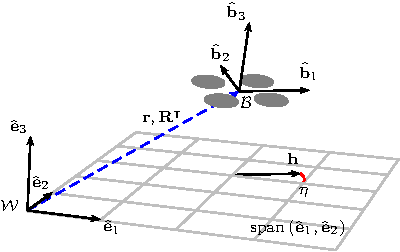
\includegraphics[width=0.90\textwidth]{fig/sketch/coordinate_frames_platform.pdf}
    % \caption{
    %   The image depicts the world frame $\mathcal{W}$ = $\{\mathbf{\hat{e}}_1$, $\mathbf{\hat{e}}_2$, $\mathbf{\hat{e}}_3\}$ in which the 3D position and the orientation of the \ac{UAV} body is expressed.
    %   The body frame $\mathcal{B}$ = $\{\mathbf{\hat{b}}_1$, $\mathbf{\hat{b}}_2$, $\mathbf{\hat{b}}_3\}$ relates to $\mathcal{W}$ by the translation $\mathbf{r} = \left[x, y, z\right]^{\intercal}$ and by rotation $\mathbf{R}^{\intercal}$.
    %   The \ac{UAV} heading vector $\mathbf{h}$, which is a projection of $\hat{\mathbf{b}}_1$ to the plane $span\left(\mathbf{\hat{e}}_1, \mathbf{\hat{e}}_2\right)$, forms the heading angle $\eta = \mathrm{atan2}\left(\mathbf{\hat{b}}_1^\intercal\mathbf{\hat{e}}_2, \mathbf{\hat{b}}_1^\intercal\mathbf{\hat{e}}_1\right) = \mathrm{atan2}\left(\mathbf{h}_{(2)}, \mathbf{h}_{(1)}\right)$.
    %   }
  \end{figure}

\end{columns}

\fullciteinbox{baca2021mrs}{}

\end{frame}

%%}

\begin{frame}
\frametitle{Reference controllers --- Desired force and heading rate}

\begin{columns}[c]

\column{0.48\textwidth} % Left column and width

\begin{block}{\small Geometric tracking on \emph{SE(3)} \cite{lee2010geometric}}
  \begin{equation}
    \scriptsize
    \begin{split}
      \mathbf{f}_d = &\overbrace{-m_e\mathbf{k}_p\circ \mathbf{e}_p}^{\begin{tabular}{c}
        \tiny position\\
        \tiny feedback
      \end{tabular}} + \overbrace{-m_e\mathbf{k}_v\circ \mathbf{e}_v}^{\begin{tabular}{c}
        \tiny velocity\\
        \tiny feedback
      \end{tabular}} + \overbrace{m_e\ddot{\mathbf{r}}_d}^{\begin{tabular}{c}
        \tiny reference\\
        \tiny feedforward
      \end{tabular}} + \\
      & \underbrace{m_eg\mathbf{\hat{e}}_3}_{\begin{tabular}{c}
        \tiny gravity\\
        \tiny compensation
      \end{tabular}} + \underbrace{-\mathbf{d}_w\circ \left[\begin{smallmatrix}
        1\\
        1\\
        0
      \end{smallmatrix}\right]}_{\begin{tabular}{c}
        \tiny world disturbance\\
        \tiny compensation
      \end{tabular}} + \underbrace{-\mathbf{d}_b\circ \left[\begin{smallmatrix}
        1\\
        1\\
        0
      \end{smallmatrix}\right]}_{\begin{tabular}{c}
        \tiny body disturbance\\
        \tiny compensation
      \end{tabular}},
    \end{split}
  \end{equation}
\end{block}

\column{0.48\textwidth} % Right column and width

\begin{block}{\small Linear MPC}
  \begin{equation}
    \scriptsize
    \begin{split}
      \mathbf{f}_d = &\overbrace{m_e\ddot{\mathbf{r}}_d}^{\begin{tabular}{c}
        \tiny reference \\
        \tiny feedforward
      \end{tabular}} + \overbrace{m_e\mathbf{c}_d}^{\begin{tabular}{c}
        \tiny MPC \\
        \tiny feedforward
      \end{tabular}} + \overbrace{m_eg\mathbf{\hat{e}}_3}^{\begin{tabular}{c}
        \tiny gravity \\
        \tiny compensation
      \end{tabular}} + \\
      &\underbrace{-\mathbf{d}_w\circ \left[\begin{smallmatrix}
        1\\
        1\\
        0
      \end{smallmatrix}\right]}_{\begin{tabular}{c}
        \tiny world disturbance\\
        \tiny compensation
      \end{tabular}} + \underbrace{-\mathbf{d}_b\circ \left[\begin{smallmatrix}
        1\\
        1\\
        0
      \end{smallmatrix}\right]}_{\begin{tabular}{c}
        \tiny body disturbance\\
        \tiny compensation
      \end{tabular}}.
    \end{split}
  \end{equation}

  \scriptsize \textbf{MPC feedforward:} desired acceleration from a constrained linear MPC.
\end{block}

\end{columns}

\fullciteinbox{baca2021mrs}{}

\end{frame}

%%}

\subsection{State estimators}

%%{ Estimator

\begin{frame}

\frametitle{The MRS UAV System}

  \begin{block}{MRS UAV System block diagram}
    \begin{figure}
      \begin{adjustbox}{max totalsize={1.0\textwidth}{.65\textheight}, center}
        \pgfdeclarelayer{foreground}
\pgfsetlayers{background,main,foreground}

\tikzset{radiation/.style={{decorate,decoration={expanding waves,angle=90,segment length=4pt}}}}

\begin{tikzpicture}[->,>=stealth', node distance=3.0cm,scale=1.0, every node/.style={scale=1.0}]

  %%{ nodes

  \node[state, shift = {(0.0, 0.0)}] (navigation) {
      \begin{tabular}{c}
        \footnotesize Trajectory \&\\
        \footnotesize generation
      \end{tabular}
    };

  % \node[state, left of = navigation, shift = {(0.5, 0.0)}] (nimbro) {
  %     \begin{tabular}{c}
  %       \footnotesize Nimbro \\
  %       \footnotesize Network
  %     \end{tabular}
  %   };

  \node[state, right of = navigation, shift = {(0.7, 0)}] (tracker) {
      \begin{tabular}{c}
        \footnotesize Reference \\
        \footnotesize tracker
      \end{tabular}
    };

  \node[state, right of = tracker, shift = {(0.1, 0)}] (controller) {
      \begin{tabular}{c}
        \footnotesize Reference \\
        \footnotesize controller
      \end{tabular}
    };

  \node[state, right of = controller, shift = {(0.8, -0)}] (attitude) {
      \begin{tabular}{c}
        \footnotesize Attitude rate\\
        \footnotesize controller
      \end{tabular}
    };

  \node[smallstate, below of = attitude, shift = {(-0.6, 2.05)}] (imu) {
      \footnotesize IMU
    };

  \node[state, right of = attitude, shift = {(0.7, -0)}] (actuators) {
      \begin{tabular}{c}
        \footnotesize UAV \\
        \footnotesize actuators
      \end{tabular}
    };

  \node[state, right of = actuators, shift = {(-0.8, -0)}] (sensors) {
      \begin{tabular}{c}
        \footnotesize Onboard \\
        \footnotesize sensors
      \end{tabular}
    };

  \node[state_focus, below of = attitude, shift = {(0, 0.9)}] (estimator) {
      \begin{tabular}{c}
        \footnotesize State \\
        \footnotesize estimator
      \end{tabular}
    };

  \node[state, right of = estimator, shift = {(0.8, 0.0)}] (localization) {
      \begin{tabular}{c}
        \footnotesize Odometry \& \\
        \footnotesize localization
      \end{tabular}
    };

  %%}

  %%{ paths

  \path[->] ($(navigation.east) + (0.0, 0)$) edge [] node[above, midway, shift = {(0.0, 0.05)}] {
      \begin{tabular}{c}
        \footnotesize desired reference\\
        \footnotesize $\mathbf{r}_d, \eta_d$\\
        \footnotesize \textit{on demand}
    \end{tabular}} ($(tracker.west) + (0.0, 0.00)$);

  % \path[->] ($(nimbro.east) + (0.0, 0)$) edge [] node[above, midway, shift = {(0.0, 0.05)}] {
  %     \begin{tabular}{c}
  %   \end{tabular}} ($(navigation.west) + (0.0, 0.00)$);

  \path[->] ($(tracker.east) + (0.0, 0)$) edge [] node[above, midway, shift = {(0.0, 0.05)}] {
      \begin{tabular}{c}
        \footnotesize full-state reference\\
        \footnotesize $\bm{\chi}_d$\\
        \footnotesize \SI{100}{\hertz}
    \end{tabular}} ($(controller.west) + (0.0, 0.00)$);

  \path[->] ($(tracker.south |- estimator.west) + (0.0, 0.0)$) edge [dotted] node[left, midway, shift = {(0.2, 0.00)}] {
      \begin{tabular}{r}
        \scriptsize initialization\\[-0.5em]
        \scriptsize only
    \end{tabular}} ($(tracker.south) + (0.0, 0.00)$);

  \path[->] ($(controller.east) + (0.0, 0)$) edge [] node[above, midway, shift = {(-0.2, 0.05)}] {
      \begin{tabular}{c}
        \footnotesize $\bm{\omega}_d$\\
        \footnotesize $T_d$ \\
        \footnotesize \SI{100}{\hertz}
    \end{tabular}} ($(attitude.west) + (0.0, 0.00)$);

  \draw[-] ($(controller.south)+(0.25,0)$) -- ($(controller.south |- estimator.west) + (0.25, 0.25)$) edge [->] node[above, near start, shift = {(-0.2, 0.05)}] {
      \begin{tabular}{c}
        \footnotesize $\mathbf{a}_d$
    \end{tabular}} ($(estimator.west) + (0, 0.25)$);

  \path[->] ($(attitude.east) + (0.0, 0)$) edge [] node[above, midway, shift = {(0.1, 0.05)}] {
      \begin{tabular}{c}
        \footnotesize $\bm{\tau}_d$ \\
        \footnotesize $\approx$\SI{1}{\kilo\hertz}
    \end{tabular}} ($(actuators.west) + (0.0, 0.00)$);

  \path[-] ($(estimator.west)+(0, 0)$) edge [] node[above, near start, shift = {(-1.0, 0.0)}] {
      \begin{tabular}{c}
        \footnotesize $\mathbf{x}$, $\mathbf{R}$, $\bm{\omega}$\\
        \footnotesize \SI{100}{\hertz}
    \end{tabular}} ($(navigation.south |- estimator.west)$) -- ($(navigation.south |- estimator.west)$) edge [->,] ($(navigation.south)+(0, 0)$);

  % \path[-] ($(estimator.west)+(0, 0)$) edge [] node[above, near start, shift = {(-1.0, 0.0)}] {
  %     \begin{tabular}{c}
  %   \end{tabular}} ($(nimbro.south |- estimator.west)$) -- ($(nimbro.south |- estimator.west)$) edge [->,] ($(nimbro.south)+(0, 0)$);

  \path[->] ($(controller.south |- estimator.west)+(0, 0)$) edge [] ($(controller.south)$);

  \draw[-] ($(imu.east) + (0.0, 0.0)$) -- ($(estimator.north |- imu.east) + (0.3, 0)$) edge [->] node[right, midway, shift = {(-0.2, 0.3)}] {
      \begin{tabular}{c}
        \footnotesize $\mathbf{R}$, $\bm{\omega}$
    \end{tabular}} ($(estimator.north) + (0.3, 0.0)$);

  \draw[-] ($(sensors.south)+(0, 0)$) -- ($(sensors.south |- localization.east)$) edge [->] ($(localization.east)$);
  \draw[-] ($(sensors.south)+(0.1, 0)$) -- ($(sensors.south |- localization.east) + (0.1, -0.1)$) edge [->] ($(localization.east) + (0.0, -0.1)$);
  \draw[-] ($(sensors.south)+(-0.1, 0)$) -- ($(sensors.south |- localization.east) + (-0.1, 0.1)$) edge [->]  ($(localization.east) + (0.0, 0.1)$);

  \draw[->] ($(localization.west)+(0, 0)$) -- ($(estimator.east)$);
  \draw[->] ($(localization.west)+(0, 0.1)$) -- ($(estimator.east) + (0, 0.1)$);
  \draw[->] ($(localization.west)+(0, -0.1)$) -- ($(estimator.east) + (0, -0.1)$);

  %%}

    % \draw[-, radiation, decoration={angle=45}] ($(nimbro.west) + (0.0, -0.0)$) -- +(0:-0.5);

  %%{ backgrounds

  \begin{pgfonlayer}{background}
    \path (attitude.west |- attitude.north)+(-0.45,0.8) node (a) {};
    \path (imu.south -| sensors.east)+(+0.25,-0.20) node (b) {};
    \path[rounded corners, draw=black!70, densely dotted]
      (a) rectangle (b);
  \end{pgfonlayer}
  \node [rectangle, above of=actuators, shift={(-0.6,0.55)}, node distance=1.7em] (autopilot) {\footnotesize UAV plant};

  \begin{pgfonlayer}{background}
    \path (attitude.west |- attitude.north)+(-0.25,0.47) node (a) {};
    \path (imu.south -| attitude.east)+(+0.25,-0.10) node (b) {};
    \path[rounded corners, draw=black!70, densely dotted]
      (a) rectangle (b);
  \end{pgfonlayer}
  \node [rectangle, above of=attitude, shift={(0,0.2)}, node distance=1.7em] (autopilot) {\footnotesize Embedded autopilot};

  %%}

\end{tikzpicture}

      \end{adjustbox}
    \end{figure}
  \end{block}

  \fullciteinbox{baca2021mrs}{}

\end{frame}

\begin{frame}

\frametitle{The MRS UAV System}

  \begin{columns}[c]

  \column{0.55\textwidth} % Left column and width

  \begin{block}{Bank of filters}

    \begin{figure}
      \begin{adjustbox}{max totalsize={1.0\textwidth}{.65\textheight}, center}
        \usetikzlibrary{shapes.geometric,backgrounds,calc,arrows}
\pgfdeclarelayer{background}
\pgfdeclarelayer{foreground}
\pgfsetlayers{background,main,foreground}

\tikzset{radiation/.style={{decorate,decoration={expanding waves,angle=90,segment length=4pt}}}}

\begin{tikzpicture}[->,>=stealth', node distance=3.0cm]

  %%{ filters

  \def\filtx{10pt}
  \def\dotoff{1.5}
  % \node[state, shift = {(0.0, 0.0)}] (preprocess) {
  %     \begin{tabular}{c}
  %       \small Preprocess
  %     \end{tabular}
  %   };

  \node[state, shift = {(0, -0)}] (k1) {
      \begin{tabular}{c}
        \small $K_1$
      \end{tabular}
    };

  \node[state, right of = k1, shift = {(-\filtx, -0)}] (k2) {
      \begin{tabular}{c}
        \small $K_2$
      \end{tabular}
    };

  \node[right of = k2, shift = {(-\dotoff, -0)}] (kdots) {
      \begin{tabular}{c}
        \small $\cdots$
      \end{tabular}
    };

  \node[state, right of = kdots, shift = {(-\dotoff, -0)}] (kn) {
      \begin{tabular}{c}
        \small $K_n$
      \end{tabular}
    };

  %%}

  %%{ predictions, corrections

  \def\eloffx{1.5}
  \def\eloffy{1.2}
  \def\ellx{20pt}
  \def\elly{22pt}
  \node[ellipse, minimum height=\elly, minimum width=\ellx, draw, above left of = k1, shift = {(\eloffx, -\eloffy)}] (pred1) {
      \small pred
    };

  \path[->] (k1.west) [bend left]  edge node {} (pred1);
  \path[->] (pred1) [bend left]  edge node {} ([xshift=-5pt]k1.north);

  \node[ellipse, minimum height=\elly, minimum width=\ellx,  draw, above right of = k1, shift = {(-\eloffx, -\eloffy)}] (corr1) {
    \small corr
  };

  \path[->] (k1.east) [bend right]  edge node {} (corr1);
  \path[->] (corr1) [bend right]  edge node {} ([xshift=5pt]k1.north);

  \node[ellipse, minimum height=\elly, minimum width=\ellx,  draw, above left of = k2, shift = {(\eloffx, -\eloffy)}] (pred2) {
    \small pred
  };

  \path[->] (k2.west) [bend left]  edge node {} (pred2);
  \path[->] (pred2) [bend left]  edge node {} ([xshift=-5pt]k2.north);

  \node[ellipse, minimum height=\elly, minimum width=\ellx,  draw, above right of = k2, shift = {(-\eloffx, -\eloffy)}] (corr2) {
    \small corr
  };

  \path[->] (k2.east) [bend right]  edge node {} (corr2);
  \path[->] (corr2) [bend right]  edge node {} ([xshift=5pt]k2.north);

  \node[ellipse, minimum height=\elly, minimum width=\ellx,  draw, above left of = kn, shift = {(\eloffx, -\eloffy)}] (predn) {
    \small pred
  };

  \path[->] (kn.west) [bend left]  edge node {} (predn);
  \path[->] (predn) [bend left]  edge node {} ([xshift=-5pt]kn.north);

  \node[ellipse, minimum height=\elly, minimum width=\ellx,  draw, above right of = kn, shift = {(-\eloffx, -\eloffy)}] (corrn) {
    \small corr
  };

  \path[->] (kn.east) [bend right]  edge node {} (corrn);
  \path[->] (corrn) [bend right]  edge node {} ([xshift=5pt]kn.north);

  %%}

  %%{ input
  
    \def\apredy{-2}
  
    \node[above of = pred1, shift = {(0, \apredy)}] (apred1) {
    };
  
    \node[above of = pred2, shift = {(0, \apredy)}] (apred2) {
    };
  
    \node[above of = predn, shift = {(0, \apredy)}] (apredn) {
    };
  
    \node[left of = apred1, shift = {(2, 0)}] (input) {
    };
  
  % node[above] {$\mathbf{T}_{total}$}
    \path[-] (input.center) edge node [above, shift = {(-0.3,0)}] {$\mathbf{u}$} (apred1.center);
    \path[-] (apred1.center) edge node {} (apred2.center);
    \path[-] (apred2.center) edge node {} (apredn.center);
  
    \path[->] (apred1.center) edge node {} (pred1.north);
    \path[->] (apred2.center) edge node {} (pred2.north);
    \path[->] (apredn.center) edge node {} (predn.north);
  
  %%}

  %%{ measurement
  
    \def\apredy{-2.2}
  
    \node[above of = corr1, shift = {(0, \apredy)}] (acorr1) {
    };
  
    \node[above of = corr2, shift = {(0, \apredy)}] (acorr2) {
    };
  
    \node[above of = corrn, shift = {(0, \apredy)}] (acorrn) {
    };
  
    \node[left of = acorr1, shift = {(1, 0)}] (measurement) {
    };
  
  % node[above] {$\mathbf{T}_{total}$}
    \path[-] (measurement.center) edge node [below, shift = {(-0.8,0)}] {$\mathbf{z}$} (acorr1.center);
    \path[-] (acorr1.center) edge node {} (acorr2.center);
    \path[-] (acorr2.center) edge node {} (acorrn.center);
  
    \path[->] (acorr1.center) edge node {} (corr1.north);
    \path[->] (acorr2.center) edge node {} (corr2.north);
    \path[->] (acorrn.center) edge node {} (corrn.north);
  
  %%}

  %%{ arbiter

  \def\mararb{5pt}
  \def\cs{5pt}
  \def\offcx{2}
  \def\offcy{1.5}

  \node[circle, inner sep=0pt, minimum size=\cs,  draw, below of = k2, shift = {(0,\offcy)}] (contact2) {
  };

  \node[circle, inner sep=0pt, minimum size=\cs,  draw, right of = contact2, shift = {(-\offcx, 0)}] (contactn) {
  };

  \node[circle, fill, inner sep=0pt, minimum size=\cs,  draw, left of = contact2, shift = {(\offcx, 0)}] (contact1) {
  };

  \def\pbky{10pt}
  \node[below of = k1, shift = {(0, 1.5*\offcy)}] (pbk1) {
  };


  \node[below of = kn, shift = {(0, 1.5*\offcy)}] (pbkn) {
  };

  \node[above of = contact1, shift = {(0, -1.5*\offcy)}] (pacontact1) {
  };

  \node[above of = contactn, shift = {(0, -1.5*\offcy)}] (pacontactn) {
  };

  % \node[circle, inner sep=0pt, minimum size=\cs,  draw, below of = contact2, shift = {(0,2.5)}] (contactb) {
  % };

  \node[below of = contact2, shift = {(0, 2.5)}] (contactb) {
  };

  \node[below of = contactb, shift = {(0, 2.5)}] (barbiter) {
  };

  \node[right of = barbiter, shift = {(0, 0)}] (estimate) {
  };

  \path[-] (k1.south) edge node {} (pbk1.center);
  \path[-] (pbk1.center) edge node {} (pacontact1.center);
\path[-] (pacontact1.center) edge node [below left, shift ={(-0.5,0.4)}] {$\mathbf{x}_1, \mathbf{\Sigma}_1$} (contact1.north);

\path[-] (k2.south) edge node [right, shift = {(0,0.34)}] {$\mathbf{x}_2, \mathbf{\Sigma}_2$} (contact2.north);

  \path[-] (kn.south) edge node {} (pbkn.center);
  \path[-] (pbkn.center) edge node {} (pacontactn.center);
\path[-] (pacontactn.center) edge node [below right, shift = {(0.5,0.4)}] {$\mathbf{x}_n, \mathbf{\Sigma}_n$} (contactn.north);

  \path[-] (contact1.south) edge node {} (contactb.center);
  \path[-,dotted] (contact2.south) edge node {} (contactb.center);
  \path[-,dotted] (contactn.south) edge node {} (contactb.center);

  \path[-] (contactb.center) edge node {} (barbiter.center);

  % \path[-] (kn.south) edge node {} (pbkn.center);
  % \path[-] (pbkn.center) edge node {} (pakn.center);
  % \path[-] (pakn.center) edge node {} (contactno.north);

  \node[state, inner sep = 0cm, minimum width=2.8cm, minimum height = 1cm, below of = k2, shift = {(-0, \offcy-0.25)}] (arbiter) {
    \begin{tabular}{ccccr}
      \\
      & & & & \small Arbiter
    \end{tabular}
  };

  %%}

  %%{ output
  
    \node[right of = barbiter, shift = {(0, 0)}] (output) {
    };
  
  % node[above] {$\mathbf{T}_{total}$}
    \path[->] (barbiter.center) edge node [above, shift = {(1,0)}] {$\mathbf{x}_{\ast }$} (output.center);
  
  
  %%}

\end{tikzpicture}

      \end{adjustbox}
    \end{figure}

  \end{block}

  \column{0.40\textwidth} % Right column and width

  \begin{itemize}
    \item simultaneous estimation of UAV state in multiple frames of reference
    \item automatic \& manual switching of the main estimator
    \item automatic detection of estimator failures
    \item switching of an estimator is synchronizes throughout the control pipeline
  \end{itemize}

  \end{columns}

  \fullciteinbox{petrlik2020robust}{}

\end{frame}

%%}

\subsection{Reference generation}

%%{ MPC Tracker

%% | ----------------------- MPC Tracker ---------------------- |

\begin{frame}
\frametitle{The MRS UAV System}

  \begin{block}{MRS UAV System block diagram}
    \begin{figure}
      \begin{adjustbox}{max totalsize={1.0\textwidth}{.65\textheight}, center}
        \pgfdeclarelayer{foreground}
\pgfsetlayers{background,main,foreground}

\tikzset{radiation/.style={{decorate,decoration={expanding waves,angle=90,segment length=4pt}}}}

\begin{tikzpicture}[->,>=stealth', node distance=3.0cm,scale=1.0, every node/.style={scale=1.0}]

  %%{ nodes

  \node[state, shift = {(0.0, 0.0)}] (navigation) {
      \begin{tabular}{c}
        \footnotesize Trajectory \&\\
        \footnotesize generation
      \end{tabular}
    };

  % \node[state, left of = navigation, shift = {(0.5, 0.0)}] (nimbro) {
  %     \begin{tabular}{c}
  %       \footnotesize Nimbro \\
  %       \footnotesize Network
  %     \end{tabular}
  %   };

  \node[state_focus, right of = navigation, shift = {(0.7, 0)}] (tracker) {
      \begin{tabular}{c}
        \footnotesize Reference \\
        \footnotesize tracker
      \end{tabular}
    };

  \node[state, right of = tracker, shift = {(0.1, 0)}] (controller) {
      \begin{tabular}{c}
        \footnotesize Reference \\
        \footnotesize controller
      \end{tabular}
    };

  \node[state, right of = controller, shift = {(0.8, -0)}] (attitude) {
      \begin{tabular}{c}
        \footnotesize Attitude rate\\
        \footnotesize controller
      \end{tabular}
    };

  \node[smallstate, below of = attitude, shift = {(-0.6, 2.05)}] (imu) {
      \footnotesize IMU
    };

  \node[state, right of = attitude, shift = {(0.7, -0)}] (actuators) {
      \begin{tabular}{c}
        \footnotesize UAV \\
        \footnotesize actuators
      \end{tabular}
    };

  \node[state, right of = actuators, shift = {(-0.8, -0)}] (sensors) {
      \begin{tabular}{c}
        \footnotesize Onboard \\
        \footnotesize sensors
      \end{tabular}
    };

  \node[state, below of = attitude, shift = {(0, 0.9)}] (estimator) {
      \begin{tabular}{c}
        \footnotesize State \\
        \footnotesize estimator
      \end{tabular}
    };

  \node[state, right of = estimator, shift = {(0.8, 0.0)}] (localization) {
      \begin{tabular}{c}
        \footnotesize Odometry \& \\
        \footnotesize localization
      \end{tabular}
    };

  %%}

  %%{ paths

  \path[->] ($(navigation.east) + (0.0, 0)$) edge [] node[above, midway, shift = {(0.0, 0.05)}] {
      \begin{tabular}{c}
        \footnotesize desired reference\\
        \footnotesize $\mathbf{r}_d, \eta_d$\\
        \footnotesize \textit{on demand}
    \end{tabular}} ($(tracker.west) + (0.0, 0.00)$);

  % \path[->] ($(nimbro.east) + (0.0, 0)$) edge [] node[above, midway, shift = {(0.0, 0.05)}] {
  %     \begin{tabular}{c}
  %   \end{tabular}} ($(navigation.west) + (0.0, 0.00)$);

  \path[->] ($(tracker.east) + (0.0, 0)$) edge [] node[above, midway, shift = {(0.0, 0.05)}] {
      \begin{tabular}{c}
        \footnotesize full-state reference\\
        \footnotesize $\bm{\chi}_d$\\
        \footnotesize \SI{100}{\hertz}
    \end{tabular}} ($(controller.west) + (0.0, 0.00)$);

  \path[->] ($(tracker.south |- estimator.west) + (0.0, 0.0)$) edge [dotted] node[left, midway, shift = {(0.2, 0.00)}] {
      \begin{tabular}{r}
        \scriptsize initialization\\[-0.5em]
        \scriptsize only
    \end{tabular}} ($(tracker.south) + (0.0, 0.00)$);

  \path[->] ($(controller.east) + (0.0, 0)$) edge [] node[above, midway, shift = {(-0.2, 0.05)}] {
      \begin{tabular}{c}
        \footnotesize $\bm{\omega}_d$\\
        \footnotesize $T_d$ \\
        \footnotesize \SI{100}{\hertz}
    \end{tabular}} ($(attitude.west) + (0.0, 0.00)$);

  \draw[-] ($(controller.south)+(0.25,0)$) -- ($(controller.south |- estimator.west) + (0.25, 0.25)$) edge [->] node[above, near start, shift = {(-0.2, 0.05)}] {
      \begin{tabular}{c}
        \footnotesize $\mathbf{a}_d$
    \end{tabular}} ($(estimator.west) + (0, 0.25)$);

  \path[->] ($(attitude.east) + (0.0, 0)$) edge [] node[above, midway, shift = {(0.1, 0.05)}] {
      \begin{tabular}{c}
        \footnotesize $\bm{\tau}_d$ \\
        \footnotesize $\approx$\SI{1}{\kilo\hertz}
    \end{tabular}} ($(actuators.west) + (0.0, 0.00)$);

  \path[-] ($(estimator.west)+(0, 0)$) edge [] node[above, near start, shift = {(-1.0, 0.0)}] {
      \begin{tabular}{c}
        \footnotesize $\mathbf{x}$, $\mathbf{R}$, $\bm{\omega}$\\
        \footnotesize \SI{100}{\hertz}
    \end{tabular}} ($(navigation.south |- estimator.west)$) -- ($(navigation.south |- estimator.west)$) edge [->,] ($(navigation.south)+(0, 0)$);

  % \path[-] ($(estimator.west)+(0, 0)$) edge [] node[above, near start, shift = {(-1.0, 0.0)}] {
  %     \begin{tabular}{c}
  %   \end{tabular}} ($(nimbro.south |- estimator.west)$) -- ($(nimbro.south |- estimator.west)$) edge [->,] ($(nimbro.south)+(0, 0)$);

  \path[->] ($(controller.south |- estimator.west)+(0, 0)$) edge [] ($(controller.south)$);

  \draw[-] ($(imu.east) + (0.0, 0.0)$) -- ($(estimator.north |- imu.east) + (0.3, 0)$) edge [->] node[right, midway, shift = {(-0.2, 0.3)}] {
      \begin{tabular}{c}
        \footnotesize $\mathbf{R}$, $\bm{\omega}$
    \end{tabular}} ($(estimator.north) + (0.3, 0.0)$);

  \draw[-] ($(sensors.south)+(0, 0)$) -- ($(sensors.south |- localization.east)$) edge [->] ($(localization.east)$);
  \draw[-] ($(sensors.south)+(0.1, 0)$) -- ($(sensors.south |- localization.east) + (0.1, -0.1)$) edge [->] ($(localization.east) + (0.0, -0.1)$);
  \draw[-] ($(sensors.south)+(-0.1, 0)$) -- ($(sensors.south |- localization.east) + (-0.1, 0.1)$) edge [->]  ($(localization.east) + (0.0, 0.1)$);

  \draw[->] ($(localization.west)+(0, 0)$) -- ($(estimator.east)$);
  \draw[->] ($(localization.west)+(0, 0.1)$) -- ($(estimator.east) + (0, 0.1)$);
  \draw[->] ($(localization.west)+(0, -0.1)$) -- ($(estimator.east) + (0, -0.1)$);

  %%}

    % \draw[-, radiation, decoration={angle=45}] ($(nimbro.west) + (0.0, -0.0)$) -- +(0:-0.5);

  %%{ backgrounds

  \begin{pgfonlayer}{background}
    \path (attitude.west |- attitude.north)+(-0.45,0.8) node (a) {};
    \path (imu.south -| sensors.east)+(+0.25,-0.20) node (b) {};
    \path[rounded corners, draw=black!70, densely dotted]
      (a) rectangle (b);
  \end{pgfonlayer}
  \node [rectangle, above of=actuators, shift={(-0.6,0.55)}, node distance=1.7em] (autopilot) {\footnotesize UAV plant};

  \begin{pgfonlayer}{background}
    \path (attitude.west |- attitude.north)+(-0.25,0.47) node (a) {};
    \path (imu.south -| attitude.east)+(+0.25,-0.10) node (b) {};
    \path[rounded corners, draw=black!70, densely dotted]
      (a) rectangle (b);
  \end{pgfonlayer}
  \node [rectangle, above of=attitude, shift={(0,0.2)}, node distance=1.7em] (autopilot) {\footnotesize Embedded autopilot};

  %%}

\end{tikzpicture}

      \end{adjustbox}
    \end{figure}
  \end{block}

  \fullciteinbox{baca2021mrs}{}

\end{frame}

\begin{frame}
\frametitle{Model Predictive Control Tracker}

\textbf{Feedback and Feed-forward multicopter controllers benefit from a smooth and feasible control reference. A step in desired position or velocity is not a feasible reference.}

\begin{columns}[c]

\column{0.48\textwidth} % Left column and width

\begin{block}{Problem}
  \begin{itemize}
    \item real-time reference generation
    \item \SI{100}{\hertz} full state reference for controllers: $\dot{\mathbf{x}}, \ddot{\mathbf{x}}, \dot{\ddot{\mathbf{x}}}$, $\ddot{\ddot{\mathbf{x}}}$, where $\mathbf{x} = \begin{pmatrix}
    r_x, r_y, r_z, \eta
    \end{pmatrix}^\intercal$ (pose and heading)
    \item UAV dynamics constraints satisfaction
    \item user input: trajectory consisting of poses sampled at regular intervals
  \end{itemize}
\end{block}

\column{0.48\textwidth} % Right column and width

\begin{block}{Solution}
  \begin{itemize}
    \item onboard real-time simulation of the linear translational UAV dynamics
    \item linear MPC (LCQP) solved at 100 Hz
    \item states of the simulated model sampled and taken as control reference
    \item \SI{8}{\second} prediction horizon used for inter-UAV collision avoidance
  \end{itemize}
\end{block}

\end{columns}

\fullciteinbox{baca2018model}{}

\end{frame}

\begin{frame}
\frametitle{Model Predictive Control Tracker}

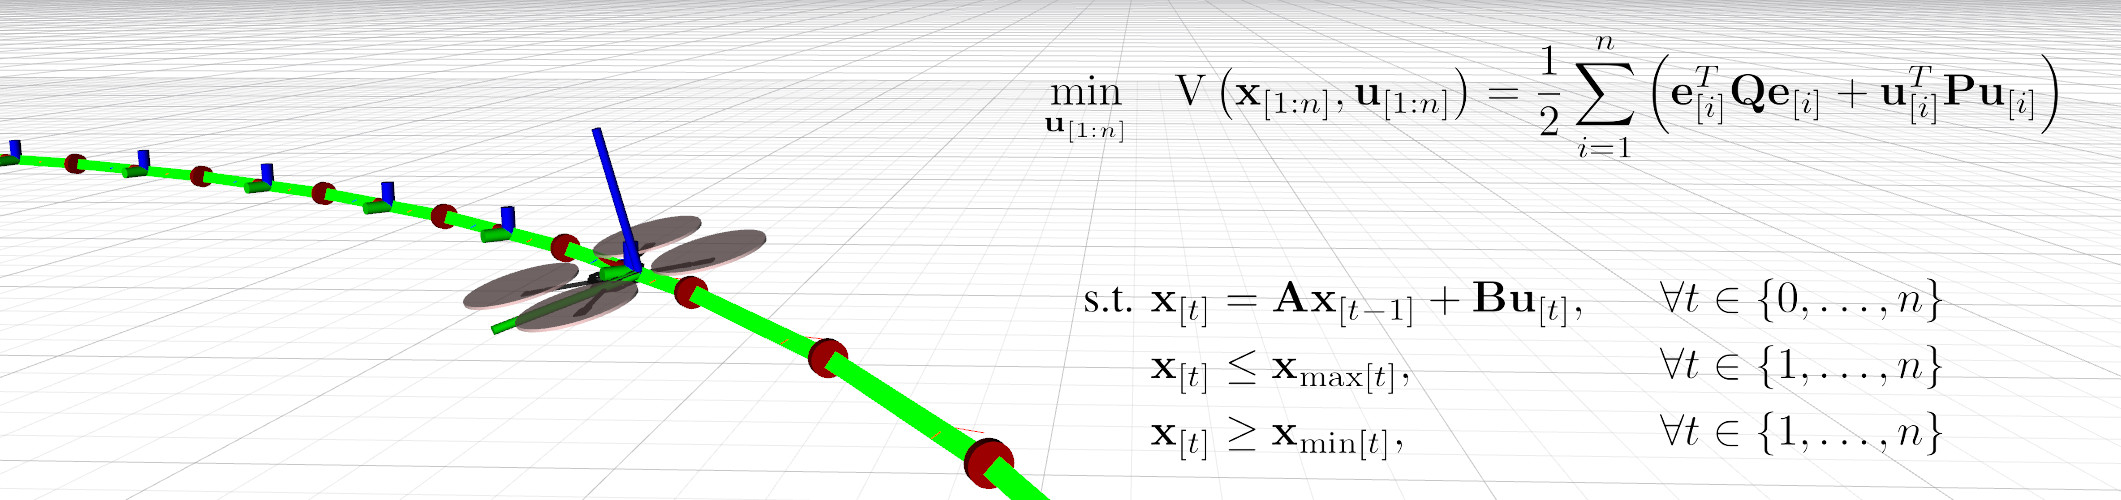
\includegraphics[width=1.0\textwidth,trim={0 0.5cm 0 1.0cm},clip]{./fig/photos/tracker.jpg}

\begin{block}{Properties}

  \vspace{-1em}

  \begin{columns}[c]

  \column{0.48\textwidth} % Left column and width

  \begin{itemize}
    \item Linear MPC is solved in real time
    \item Mutual collision avoidance prevent damage during experimentation
  \end{itemize}

  \column{0.48\textwidth} % Right column and width
  \begin{itemize}
    \item The LCQP can be solved reliably
    \item The tracker can handle unfeasible trajectory references from a user
  \end{itemize}

  \end{columns}

\end{block}

% \fullciteinbox{baca2018model}{http://github.com/ctu-mrs/mrs_uav_trackers}
\fullciteinbox{baca2018model}{}

\end{frame}

%%}

%%%{ control performance showcase

%\begin{frame}
%\frametitle{Showcase of the capabilities}

%\only<1>{
%  \begin{block}{Aggressive trajectory following}
%    \begin{center}
%      \mymovie[autostart,loop,start=30]{
%        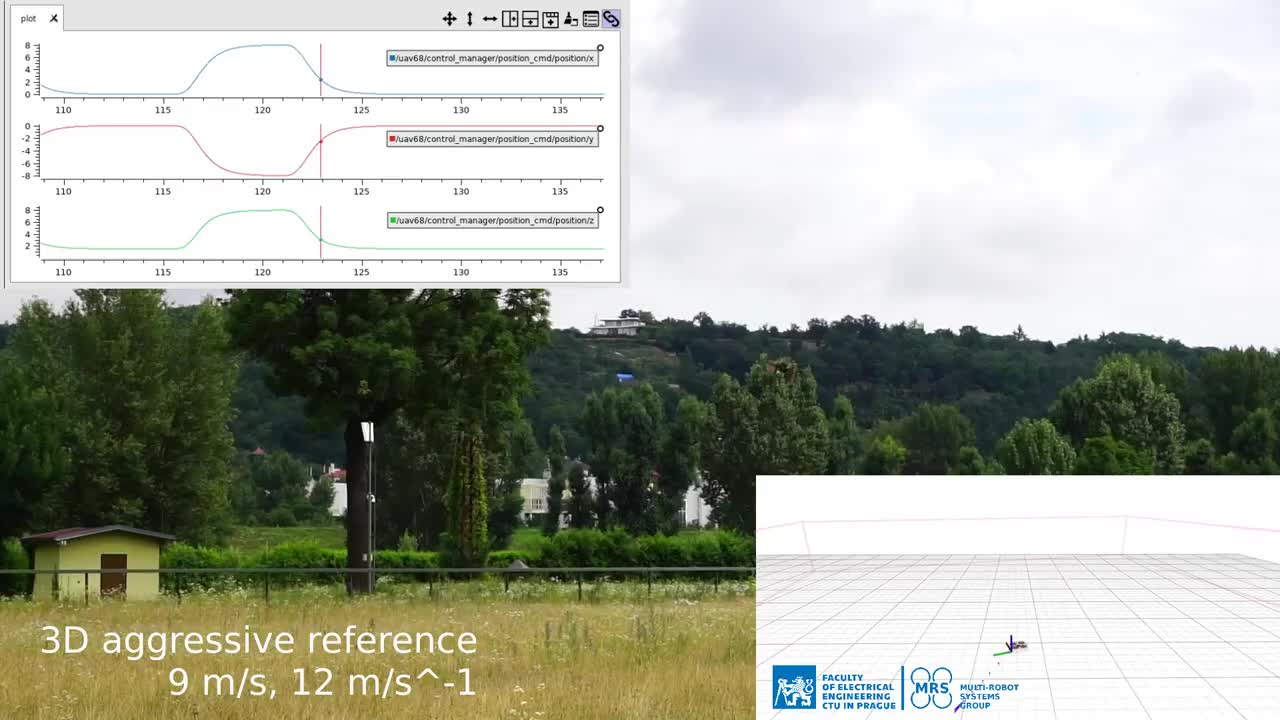
\includegraphics[width=0.7\textwidth]{./fig/mrs_uav_system_thumbnail.jpg}
%      }{./videos/mrs_uav_system.mp4}\\
%      Video: \url{http://mrs.felk.cvut.cz/mrs-uav-system}
%    \end{center}
%  \end{block}
%}

%\only<2>{
%  \begin{block}{Flip}
%    \begin{center}
%      \mymovie[autostart,loop]{
%        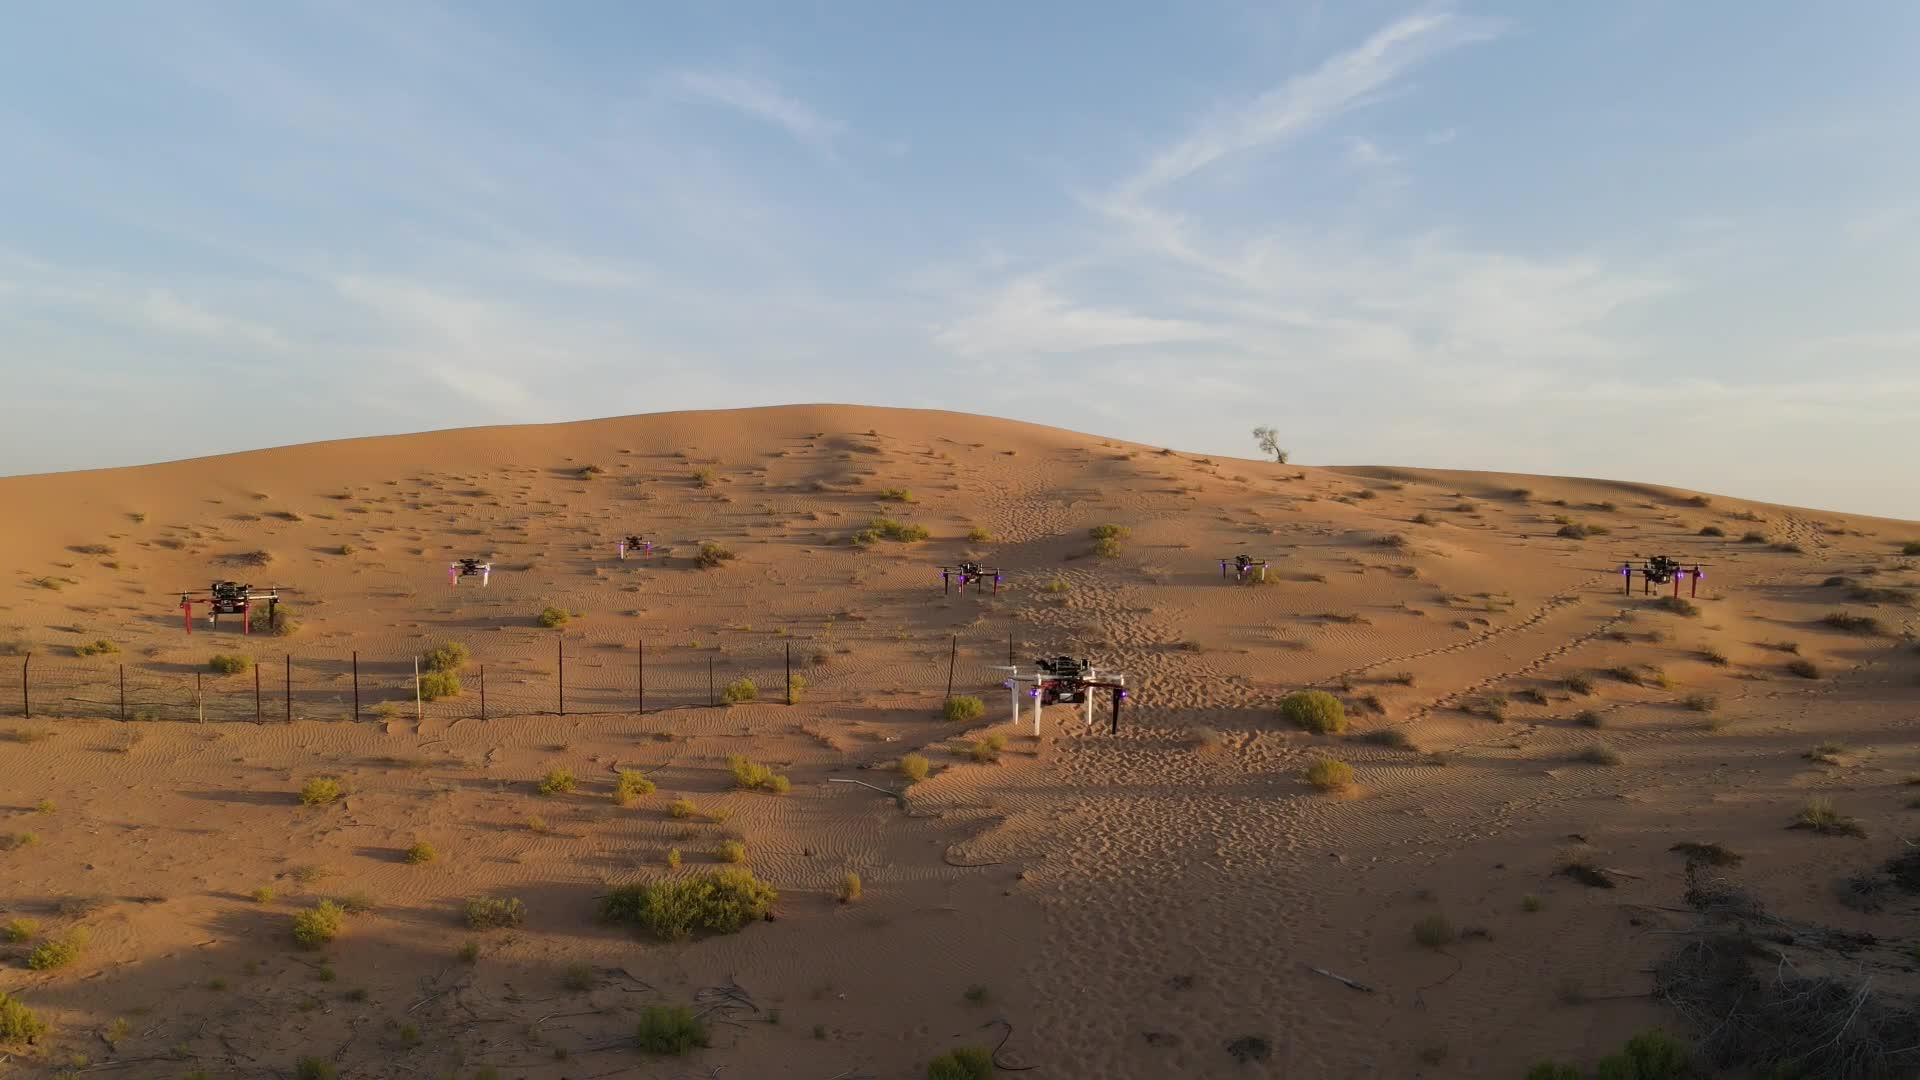
\includegraphics[width=0.8\textwidth]{./fig/flip_thumbnail.jpg}
%      }{./videos/flip.mp4}\\
%    \end{center}
%  \end{block}
%}

%\end{frame}

%%%}

\subsection{Trajectory generation}

%%{ Trajectory generation

\begin{frame}
\frametitle{Trajectory Generation}

  \begin{block}{MRS UAV System block diagram}
    \begin{figure}
      \begin{adjustbox}{max totalsize={1.0\textwidth}{.65\textheight}, center}
        \pgfdeclarelayer{foreground}
\pgfsetlayers{background,main,foreground}

\tikzset{radiation/.style={{decorate,decoration={expanding waves,angle=90,segment length=4pt}}}}

\begin{tikzpicture}[->,>=stealth', node distance=3.0cm,scale=1.0, every node/.style={scale=1.0}]

  %%{ nodes

  \node[state_focus, shift = {(0.0, 0.0)}] (navigation) {
      \begin{tabular}{c}
        \footnotesize Trajectory \&\\
        \footnotesize generation
      \end{tabular}
    };

  % \node[state, left of = navigation, shift = {(0.5, 0.0)}] (nimbro) {
  %     \begin{tabular}{c}
  %       \footnotesize Nimbro \\
  %       \footnotesize Network
  %     \end{tabular}
  %   };

  \node[state, right of = navigation, shift = {(0.7, 0)}] (tracker) {
      \begin{tabular}{c}
        \footnotesize Reference \\
        \footnotesize tracker
      \end{tabular}
    };

  \node[state, right of = tracker, shift = {(0.1, 0)}] (controller) {
      \begin{tabular}{c}
        \footnotesize Reference \\
        \footnotesize controller
      \end{tabular}
    };

  \node[state, right of = controller, shift = {(0.8, -0)}] (attitude) {
      \begin{tabular}{c}
        \footnotesize Attitude rate\\
        \footnotesize controller
      \end{tabular}
    };

  \node[smallstate, below of = attitude, shift = {(-0.6, 2.05)}] (imu) {
      \footnotesize IMU
    };

  \node[state, right of = attitude, shift = {(0.7, -0)}] (actuators) {
      \begin{tabular}{c}
        \footnotesize UAV \\
        \footnotesize actuators
      \end{tabular}
    };

  \node[state, right of = actuators, shift = {(-0.8, -0)}] (sensors) {
      \begin{tabular}{c}
        \footnotesize Onboard \\
        \footnotesize sensors
      \end{tabular}
    };

  \node[state, below of = attitude, shift = {(0, 0.9)}] (estimator) {
      \begin{tabular}{c}
        \footnotesize State \\
        \footnotesize estimator
      \end{tabular}
    };

  \node[state, right of = estimator, shift = {(0.8, 0.0)}] (localization) {
      \begin{tabular}{c}
        \footnotesize Odometry \& \\
        \footnotesize localization
      \end{tabular}
    };

  %%}

  %%{ paths

  \path[->] ($(navigation.east) + (0.0, 0)$) edge [] node[above, midway, shift = {(0.0, 0.05)}] {
      \begin{tabular}{c}
        \footnotesize desired reference\\
        \footnotesize $\mathbf{r}_d, \eta_d$\\
        \footnotesize \textit{on demand}
    \end{tabular}} ($(tracker.west) + (0.0, 0.00)$);

  % \path[->] ($(nimbro.east) + (0.0, 0)$) edge [] node[above, midway, shift = {(0.0, 0.05)}] {
  %     \begin{tabular}{c}
  %   \end{tabular}} ($(navigation.west) + (0.0, 0.00)$);

  \path[->] ($(tracker.east) + (0.0, 0)$) edge [] node[above, midway, shift = {(0.0, 0.05)}] {
      \begin{tabular}{c}
        \footnotesize full-state reference\\
        \footnotesize $\bm{\chi}_d$\\
        \footnotesize \SI{100}{\hertz}
    \end{tabular}} ($(controller.west) + (0.0, 0.00)$);

  \path[->] ($(tracker.south |- estimator.west) + (0.0, 0.0)$) edge [dotted] node[left, midway, shift = {(0.2, 0.00)}] {
      \begin{tabular}{r}
        \scriptsize initialization\\[-0.5em]
        \scriptsize only
    \end{tabular}} ($(tracker.south) + (0.0, 0.00)$);

  \path[->] ($(controller.east) + (0.0, 0)$) edge [] node[above, midway, shift = {(-0.2, 0.05)}] {
      \begin{tabular}{c}
        \footnotesize $\bm{\omega}_d$\\
        \footnotesize $T_d$ \\
        \footnotesize \SI{100}{\hertz}
    \end{tabular}} ($(attitude.west) + (0.0, 0.00)$);

  \draw[-] ($(controller.south)+(0.25,0)$) -- ($(controller.south |- estimator.west) + (0.25, 0.25)$) edge [->] node[above, near start, shift = {(-0.2, 0.05)}] {
      \begin{tabular}{c}
        \footnotesize $\mathbf{a}_d$
    \end{tabular}} ($(estimator.west) + (0, 0.25)$);

  \path[->] ($(attitude.east) + (0.0, 0)$) edge [] node[above, midway, shift = {(0.1, 0.05)}] {
      \begin{tabular}{c}
        \footnotesize $\bm{\tau}_d$ \\
        \footnotesize $\approx$\SI{1}{\kilo\hertz}
    \end{tabular}} ($(actuators.west) + (0.0, 0.00)$);

  \path[-] ($(estimator.west)+(0, 0)$) edge [] node[above, near start, shift = {(-1.0, 0.0)}] {
      \begin{tabular}{c}
        \footnotesize $\mathbf{x}$, $\mathbf{R}$, $\bm{\omega}$\\
        \footnotesize \SI{100}{\hertz}
    \end{tabular}} ($(navigation.south |- estimator.west)$) -- ($(navigation.south |- estimator.west)$) edge [->,] ($(navigation.south)+(0, 0)$);

  % \path[-] ($(estimator.west)+(0, 0)$) edge [] node[above, near start, shift = {(-1.0, 0.0)}] {
  %     \begin{tabular}{c}
  %   \end{tabular}} ($(nimbro.south |- estimator.west)$) -- ($(nimbro.south |- estimator.west)$) edge [->,] ($(nimbro.south)+(0, 0)$);

  \path[->] ($(controller.south |- estimator.west)+(0, 0)$) edge [] ($(controller.south)$);

  \draw[-] ($(imu.east) + (0.0, 0.0)$) -- ($(estimator.north |- imu.east) + (0.3, 0)$) edge [->] node[right, midway, shift = {(-0.2, 0.3)}] {
      \begin{tabular}{c}
        \footnotesize $\mathbf{R}$, $\bm{\omega}$
    \end{tabular}} ($(estimator.north) + (0.3, 0.0)$);

  \draw[-] ($(sensors.south)+(0, 0)$) -- ($(sensors.south |- localization.east)$) edge [->] ($(localization.east)$);
  \draw[-] ($(sensors.south)+(0.1, 0)$) -- ($(sensors.south |- localization.east) + (0.1, -0.1)$) edge [->] ($(localization.east) + (0.0, -0.1)$);
  \draw[-] ($(sensors.south)+(-0.1, 0)$) -- ($(sensors.south |- localization.east) + (-0.1, 0.1)$) edge [->]  ($(localization.east) + (0.0, 0.1)$);

  \draw[->] ($(localization.west)+(0, 0)$) -- ($(estimator.east)$);
  \draw[->] ($(localization.west)+(0, 0.1)$) -- ($(estimator.east) + (0, 0.1)$);
  \draw[->] ($(localization.west)+(0, -0.1)$) -- ($(estimator.east) + (0, -0.1)$);

  %%}

    % \draw[-, radiation, decoration={angle=45}] ($(nimbro.west) + (0.0, -0.0)$) -- +(0:-0.5);

  %%{ backgrounds

  \begin{pgfonlayer}{background}
    \path (attitude.west |- attitude.north)+(-0.45,0.8) node (a) {};
    \path (imu.south -| sensors.east)+(+0.25,-0.20) node (b) {};
    \path[rounded corners, draw=black!70, densely dotted]
      (a) rectangle (b);
  \end{pgfonlayer}
  \node [rectangle, above of=actuators, shift={(-0.6,0.55)}, node distance=1.7em] (autopilot) {\footnotesize UAV plant};

  \begin{pgfonlayer}{background}
    \path (attitude.west |- attitude.north)+(-0.25,0.47) node (a) {};
    \path (imu.south -| attitude.east)+(+0.25,-0.10) node (b) {};
    \path[rounded corners, draw=black!70, densely dotted]
      (a) rectangle (b);
  \end{pgfonlayer}
  \node [rectangle, above of=attitude, shift={(0,0.2)}, node distance=1.7em] (autopilot) {\footnotesize Embedded autopilot};

  %%}

\end{tikzpicture}

      \end{adjustbox}
    \end{figure}
  \end{block}

  \fullciteinbox{baca2021mrs}{}

\end{frame}

\begin{frame}
\frametitle{Trajectory Generation}

\begin{block}{Path $\rightarrow$ Feasible Trajectory}
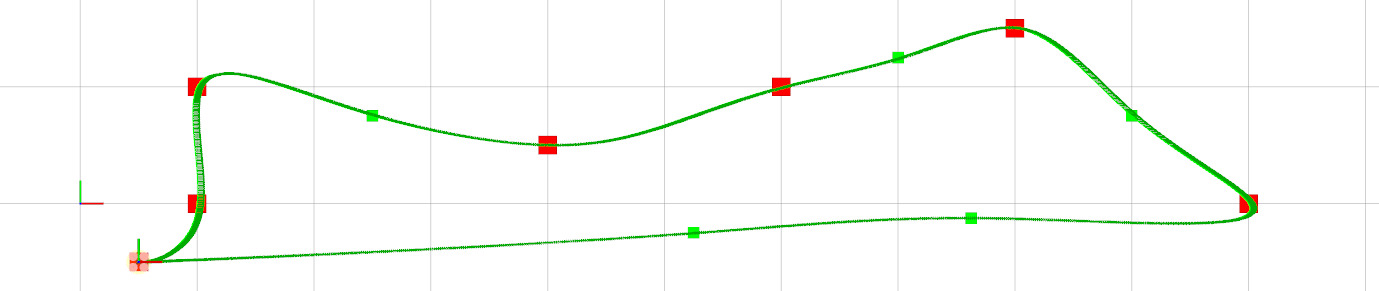
\includegraphics[width=0.9\textwidth]{./fig/trajectory_generation.jpg}
\end{block}

\begin{center}
  Fork of {\color{blue} ethz-asl/mav\_trajectory\_generation}
\end{center}

\fullciteinbox{richter2016polynomial}{}
\fullciteinbox{burri2015realtime}{}

\end{frame}

\begin{frame}
\frametitle{Trajectory Generation --- Improvements and beyond}

\begin{itemize}
  \item fixed poorly-implemented lower bound segment time initialization
  \item fixed poorly-implemented trajectory sampling
  \item recursive segment sub-sectioning for meeting desired corridor constraints
  \item + smooth continuation of the prior UAV motion (Requires the \emph{MPC Tracker})
  \item + Fallback solution if the \texttt{QP} optimization fails
  \item + asynchronous execution and timeouting (with fallback solution)
  \item + result sanitization
\end{itemize}

\fullciteinbox{baca2021mrs}{}

\end{frame}

% \begin{frame}
% \frametitle{Trajectory Generation}

% \begin{block}{DARPA SubT Virtual - 2017--2021}
%   \begin{center}
%     \mymovie[autostart,loop]{
%       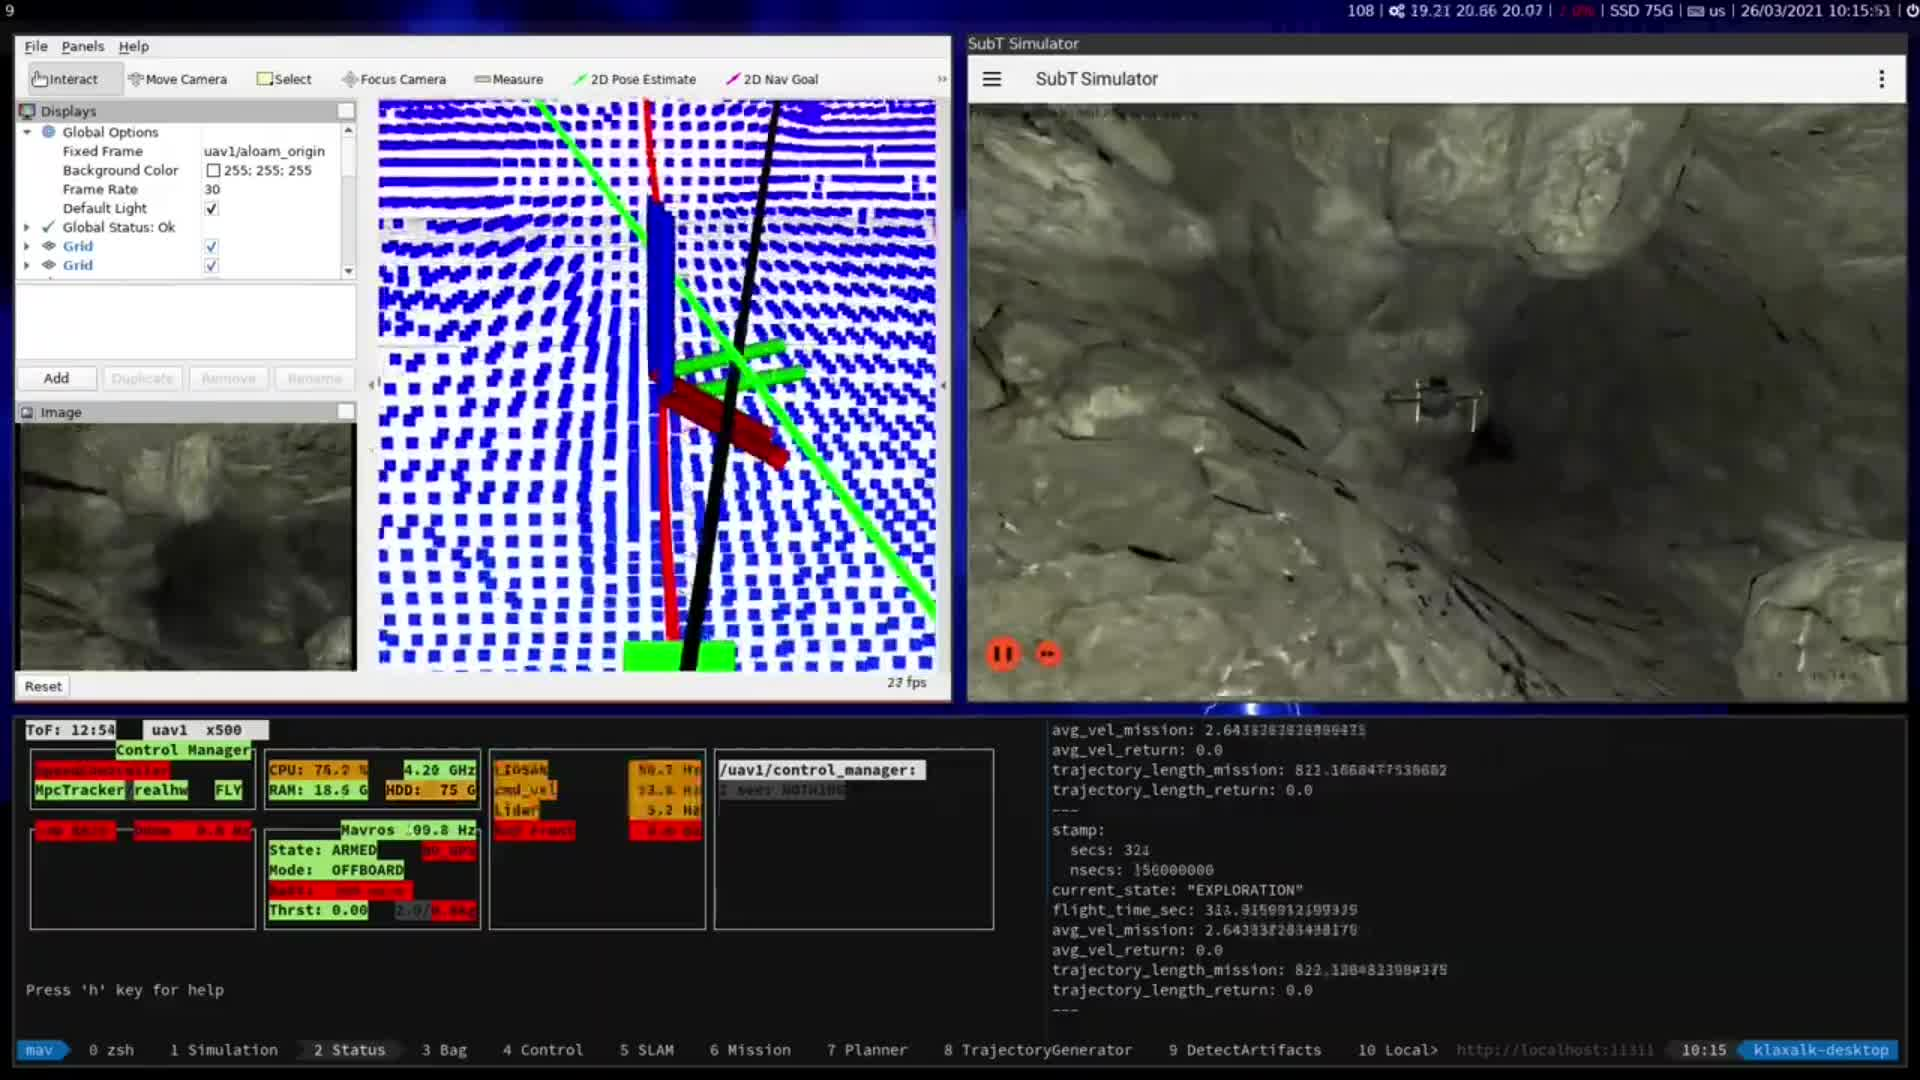
\includegraphics[width=0.8\textwidth]{./fig/darpa_virtual_cave_thumbnail.jpg}
%     }{./videos/darpa_virtual_cave_short.mp4}\\
%   \end{center}
% \end{block}

% \end{frame}

%%}

%%{ ROS -- Robot Operating System

\begin{frame}
  \frametitle{ROS -- Robot Operating System}

  \begin{itemize}
    \item middleware allowing communication between programs
    \item integrates with \texttt{C++}, Python, Bash and Zshell
    \item makes the transition from \emph{theory} to \emph{bare metal} bearable
    \item universally supported by sensor manufacturers
    \item used globally by the research community
    \item integration through the Linux terminal
    \item out of the box: time and clock management, logging, recording onboard data, visualization and plotting, parameter loading, static and dynamic transformations, etc.
    \item integrates to robotic simulators: Gazebo, Coppelia (V-REP), AirSim
  \end{itemize}

  \begin{figure}
    
\includegraphics[width=0.3\textwidth]{fig/ros_logo.jpg}
  \end{figure}

\end{frame}

%%}

%%{ Implementation diagram

\begin{frame}
\frametitle{Modularity and abstractions}

\begin{columns}[c]

\column{0.48\textwidth} % Left column and width

\begin{itemize}
  \item Modularity promotes collaborative development
  \item Modularity leads to separation of concerns
  \item Allows component substitution and mocking
  \item Makes building abstract interfaces easier
  \item Allows for distributed execution across more machines
  \item Makes introspection easier
  \item {\color{red} makes runtime performance worse}
  \item {\color{red} proper data exchange is major part of the system design}
\end{itemize}

\column{0.48\textwidth} % Right column and width

\begin{block}{Modular system architecture}
  \begin{adjustbox}{max totalsize={1.0\textwidth}{.65\textheight}, center}
    \pgfdeclarelayer{foreground}
\pgfsetlayers{background,main,foreground}

\tikzset{radiation/.style={{decorate,decoration={expanding waves,angle=90,segment length=0.1em}}}}

\begin{tikzpicture}[->,>=stealth', node distance=7.0em]

  %%{ nodes

  \node[state_blue, shift = {(0.0em, 0.0em)}] (control_manager) {
    \begin{tabular}{c}
      \scriptsize Control manager
    \end{tabular}
  };

  \node[state_red, right of = control_manager, shift = {(2.0em, 0.0em)}] (mpc_tracker) {
    \begin{tabular}{c}
      \scriptsize MPC tracker
    \end{tabular}
  };

  \node[state_red, below of = mpc_tracker, shift = {(0.0em, 4.5em)}] (landoff_tracker) {
    \begin{tabular}{c}
      \scriptsize Landoff tracker
    \end{tabular}
  };

  \node[state_blue, above of = mpc_tracker, shift = {(0.0em, -4.0em)}] (constraint_manager) {
    \begin{tabular}{c}
      \scriptsize Constraint manager
    \end{tabular}
  };

  \node[state_blue, above of = constraint_manager,  shift = {(-1.0em, -4.5em)}] (uav_manager) {
    \begin{tabular}{c}
      \scriptsize UAV manager
    \end{tabular}
  };

  \node[state_red, below of = landoff_tracker, shift = {(0.0em, 4.5em)}] (speed_tracker) {
    \begin{tabular}{c}
      \scriptsize Speed tracker
    \end{tabular}
  };

  \node[below of = speed_tracker, shift = {(0.0em, 4.5em)}] (dots_tracker) {
    \begin{tabular}{c}
      $\vdots$
    \end{tabular}
  };

  \node[state_green, left of = control_manager, shift = {(-2.0em, 0.0em)}] (se3_controller) {
    \begin{tabular}{c}
      \scriptsize SE(3) controller
    \end{tabular}
  };

  \node[state_green, below of = se3_controller, shift = {(0.0em, 4.5em)}] (mpc_controller) {
    \begin{tabular}{c}
      \scriptsize MPC controller
    \end{tabular}
  };

  \node[state_blue, above of = se3_controller, shift = {(0.0em, -4.0em)}] (gain_manager) {
    \begin{tabular}{c}
      \scriptsize Gain manager
    \end{tabular}
  };

  \node[state_green, below of = mpc_controller, shift = {(0.0em, 4.5em)}] (failsafe_controller) {
    \begin{tabular}{c}
      \scriptsize Failsafe controller
    \end{tabular}
  };

  \node[below of = failsafe_controller, shift = {(0.0em, 4.5em)}] (dots_controller) {
    \begin{tabular}{c}
      $\vdots$
    \end{tabular}
  };

  \node[state_white, below of = control_manager, shift = {(0.0em, 4.2em)}] (mavros2) {
    \begin{tabular}{c}
      \scriptsize HW API
    \end{tabular}
  };

  % \node[state_white, above of = control_manager, shift = {(-2.2em, -3.0em)}] (nimbro) {
  %     \begin{tabular}{c}
  %       \scriptsize Nimbro
  %     \end{tabular}
  %   };

  \node[state_gray, below of = mavros2, shift = {(0.0em, 4.2em)}] (pixhawk2) {
    \begin{tabular}{c}
      \scriptsize UAV HW
    \end{tabular}
  };

  \node[state_white, above of = control_manager, shift = {(0.0em, 0.0em)}] (estimator) {
    \begin{tabular}{c}
      \scriptsize Estimation manager
    \end{tabular}
  };

  \node[state_white, above of = estimator, shift = {(0.0em, -4.0em)}] (mavros) {
    \begin{tabular}{c}
      \scriptsize Mavros
    \end{tabular}
  };

  \node[state_gray, above of = mavros, shift = {(0.0em, -4.0em)}] (pixhawk) {
    \begin{tabular}{c}
      \scriptsize Pixhawk
    \end{tabular}
  };

  \node[state_white, right of = mavros, shift = {(-1.4em, 0.0em)}] (optic_flow) {
    \begin{tabular}{c}
      \scriptsize Optic flow
    \end{tabular}
  };

  \node[state_gray, above of = optic_flow, shift = {(0.0em, -4.0em)}] (camera) {
    \begin{tabular}{c}
      \scriptsize Camera
    \end{tabular}
  };

  \node[state_gray, left of = mavros, shift = {(0.8em, 0.0em)}] (height) {
    \begin{tabular}{c}
      \scriptsize Height sensor
    \end{tabular}
  };

  \node[state_gray, left of = height, shift = {(0.3em, 0.0em)}] (rtk) {
    \begin{tabular}{c}
      \scriptsize RTK GPS
    \end{tabular}
  };

  \node[state_white, right of = optic_flow, shift = {(-1.5em, 0.0em)}] (slam) {
    \begin{tabular}{c}
      \scriptsize SLAM
    \end{tabular}
  };

  \node[state_gray, above of = slam, shift = {(0.0em, -4.0em)}] (lidar) {
    \begin{tabular}{c}
      \scriptsize LIDAR
    \end{tabular}
  };

  %%}

  %%{ paths

  %% | ------------ connected sensor data to estimator ----------- |
  \path[-] ($(rtk.south)$) edge [->] ($(estimator.north) + (-2em, 0)$);
  \path[-] ($(height.south)$) edge [->] ($(estimator.north) + (-1.0em, 0)$);
  \path[-] ($(optic_flow.south)$) edge [->] ($(estimator.north) + (1.0em, 0)$);
  \path[-] ($(slam.south)$) edge [->] ($(estimator.north) + (2em, 0)$);
  \path[-] ($(mavros.south)$) edge [->] ($(estimator.north) + (0em, 0)$);

  \path[] ($(camera.south)$) edge [->] ($(optic_flow.north)$);

  %% | ---------------------- lidar to slam --------------------- |
  \path[-] ($(slam.north |- lidar.south)$) edge [->] ($(slam.north)$);

  %% | ----- connections from controllers to control manager ---- |
  \path ($(se3_controller.east)$) edge [<->] ($(control_manager.west) + (0, 0.4em)$);
  \path ($(mpc_controller.east)$) edge [<->] ($(control_manager.west) + (0, 0.20em)$);
  \path ($(failsafe_controller.east)$) edge [<->] ($(control_manager.west) + (0, 0.0em)$);
  % \path ($(failsafe_controller.east |- dots_controller.east)$) edge [<->] ($(control_manager.west) + (0, -0.2em)$);

  %% | ------ connections from trackers to control manager ------ |
  \path ($(speed_tracker.west)$) edge [<->] ($(control_manager.east) + (0, 0.00em)$);
  \path ($(landoff_tracker.west)$) edge [<->] ($(control_manager.east) + (0, 0.20em)$);
  \path ($(mpc_tracker.west)$) edge [<->] ($(control_manager.east) + (0, 0.40em)$);
  % \path ($(speed_tracker.west |- dots_tracker.west)$) edge [<->] ($(control_manager.east) + (0, -0.20em)$);

  %% | ------------------- gain manager to se3 ------------------ |
  \path[-] ($(gain_manager.south)$) edge [->] ($(se3_controller.north)$);

  %% | ---------- constraint manager to control manager --------- |
  \draw[-] ($(constraint_manager.west)$) -- ($(control_manager.north |- constraint_manager.west) + (2em, 0)$) edge [->] ($(control_manager.north) + (2em, 0)$);

  %% | ------------- control manager to uav manager ------------- |
  \draw[-] ($(uav_manager.west)$) -- ($(control_manager.north |- uav_manager.west) + (1em, 0)$) edge [->] ($(control_manager.north) + (1em, 0)$);

  %% | --------------- estimator to control manager -------------- |
  \path ($(estimator.south) + (0.0em, 0)$) edge [->] ($(control_manager.north) + (0.0em, 0)$);

  %% | --------------- estimator to uav manager -------------- |
  \draw[-] ($(estimator.east)$) -- ($(uav_manager.north |- estimator.east) + (0em, 0)$) edge [->] ($(uav_manager.north) + (0em, 0)$);

  %% | ---------------- estimator to gain manager --------------- |
  \draw[-] ($(estimator.west)$) -- ($(gain_manager.north |- estimator.west) + (0em, 0)$) edge [->] ($(gain_manager.north) + (0em, 0)$);

  %% | ------------- estimator to constraint manager ------------ |
  \draw[-] ($(estimator.east)$) -- ($(constraint_manager.north |- estimator.east) + (2.5em, 0)$) edge [->] ($(constraint_manager.north) + (2.5em, 0)$);

  %% | ------------------------- pixhawk ------------------------ |
  \path ($(pixhawk.south)$) edge [->] ($(mavros.north)$);

  %% | ------------------------ pixhawk 2 ----------------------- |
  \path ($(mavros2.north |- control_manager.south)$) edge [->] ($(mavros2.north)$);
  \path ($(pixhawk2.north)$) edge [<-] ($(mavros2.south)$);

  % %% | ------------------------- nimbro ------------------------- |
  % \path ($(nimbro.south)$) edge [->] ($(nimbro.south |- control_manager.north)$);

  %%}

  %%{ backgrounds

  % \begin{pgfonlayer}{background}
  %   \path (se3_controller.east |- se3_controller.north)+(+0.3, 0.3) node (a) {};
  %   \path (attitude_controller.south -| se3_controller.west)+(-0.3,-0.3) node (b) {};
  %   \path[fill=black!70, draw=black!50, dashed]
  %   (a) rectangle (b);
  %   \path (a) -- node [midway, shift = {(-5.5, -1.0)}] {\begin{tabular}{c}
  %       \scriptsize Controllers\\
  %       \scriptsize (ROS Plugins)
  %   \end{tabular}} (a);
  % \end{pgfonlayer}

  % \begin{pgfonlayer}{background}
  %   \path (landoff_tracker.east |- landoff_tracker.north)+(+0.3, 0.3) node (a) {};
  %   \path (csv_tracker.south -| landoff_tracker.west)+(-0.3,-0.3) node (b) {};
  %   \path[fill=black!70, draw=black!50, dashed]
  %   (a) rectangle (b);
  %   \path (a) -- node [midway, shift = {(1.5, -1.0)}] {\begin{tabular}{c}
  %       \scriptsize Trackers\\
  %       \scriptsize (ROS Plugins)
  %   \end{tabular}} (a);
  % \end{pgfonlayer}

  %%}

\end{tikzpicture}

  \end{adjustbox}
\end{block}

\end{columns}

\end{frame}

% \begin{frame}
% \frametitle{Full implementation diagram}

%   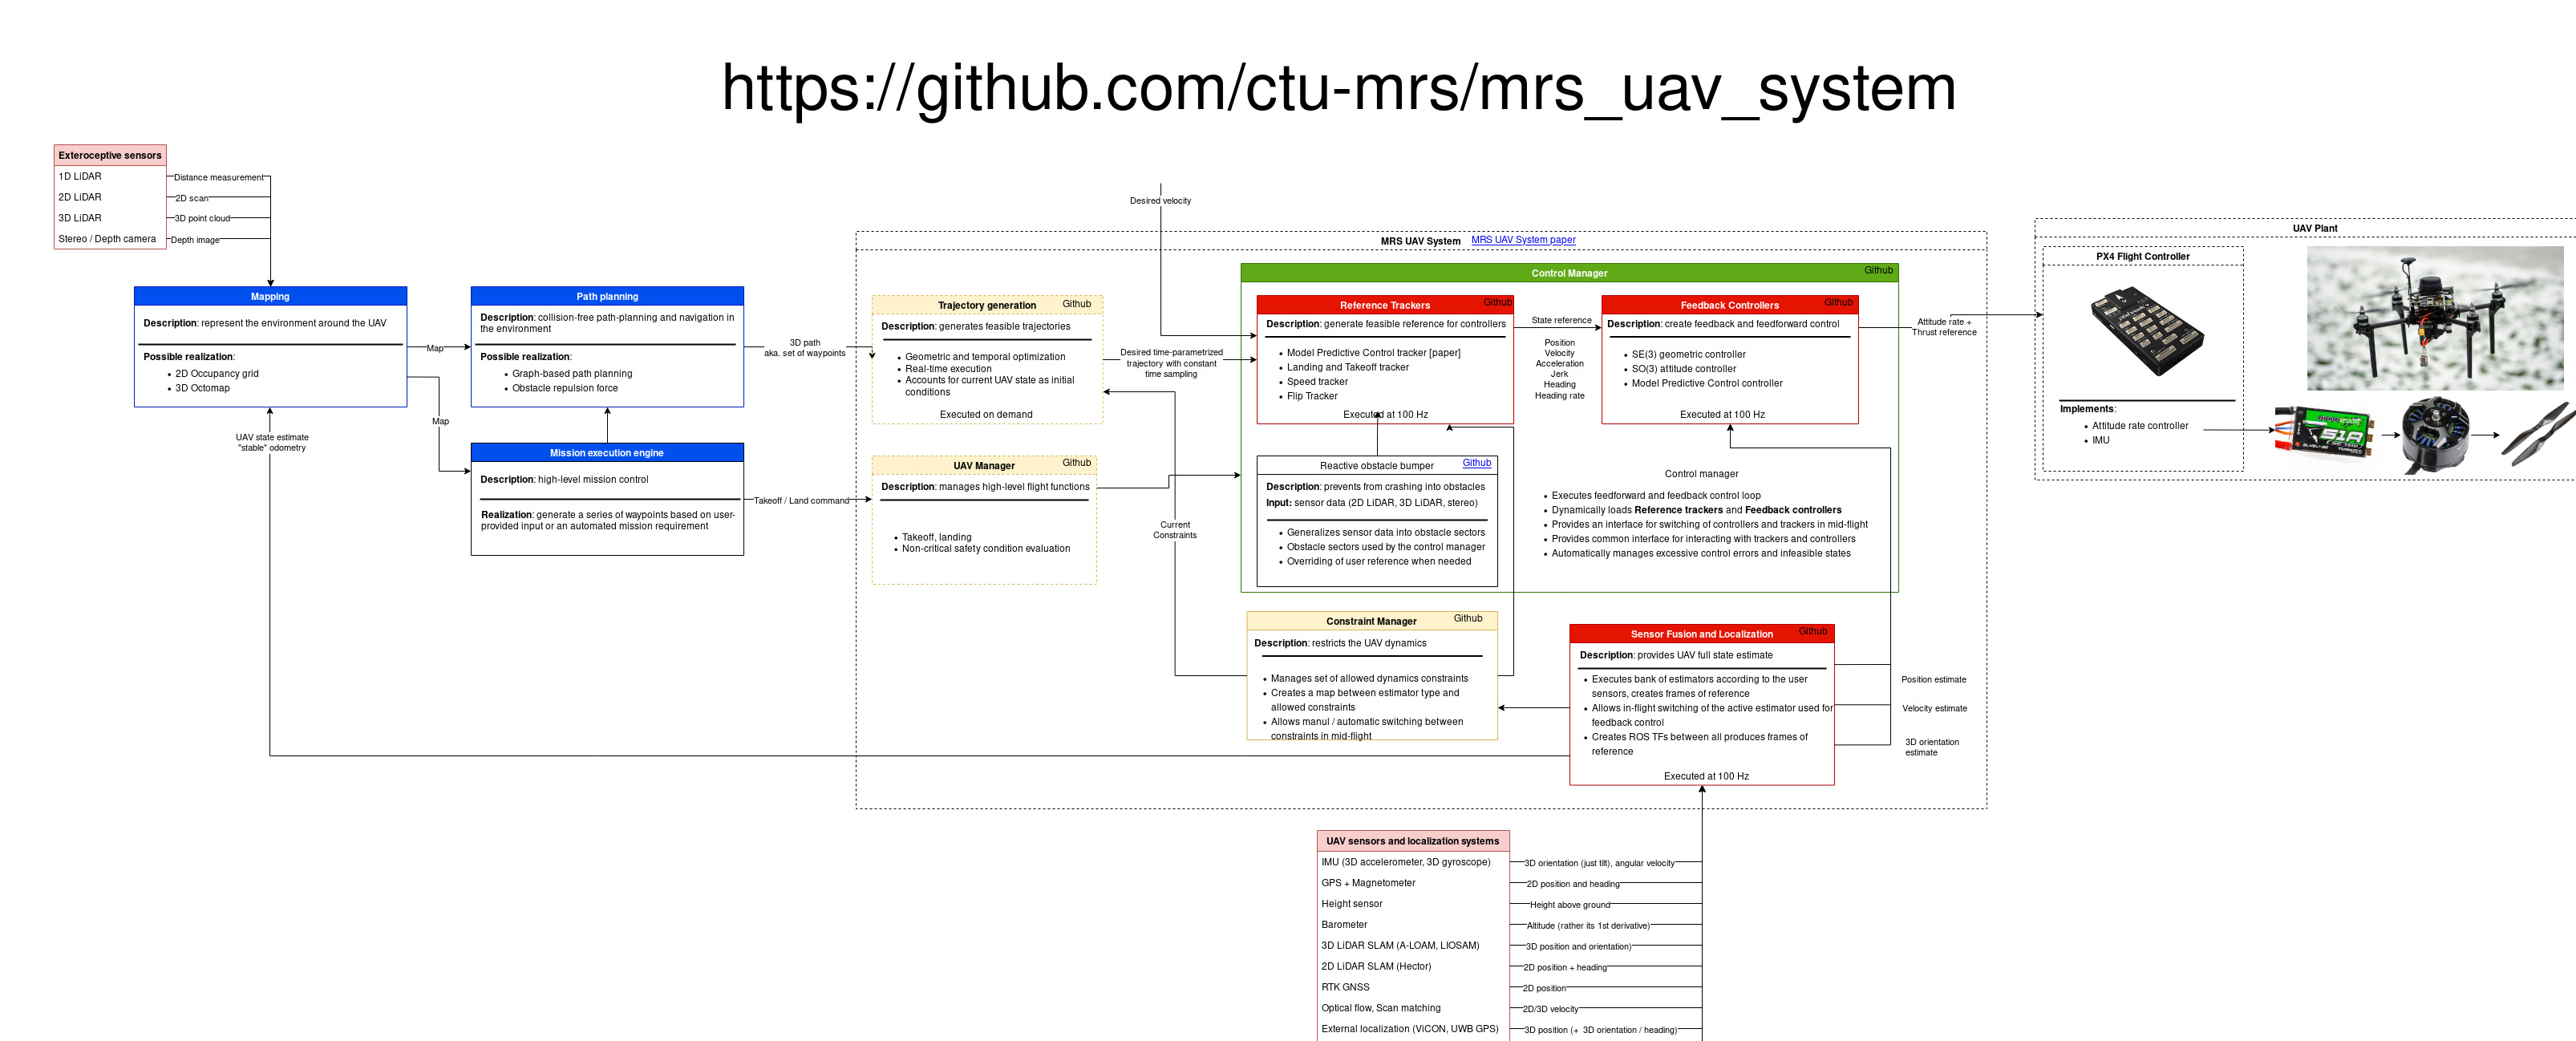
\includegraphics[width=1.0\textwidth]{./fig/full_diagram.jpg}

% \end{frame}

%%}

\subsection{Mapping and planning}

  %%{ Mapping Planning

  \begin{frame}
    \frametitle{Mapping \& Planning Pipeline}

    \begin{block}{Realtime Mapping \& Planning pipeline using LiDAR, RGBD}
      \begin{center}
        \mymovie[autostart,loop,start=58]{
          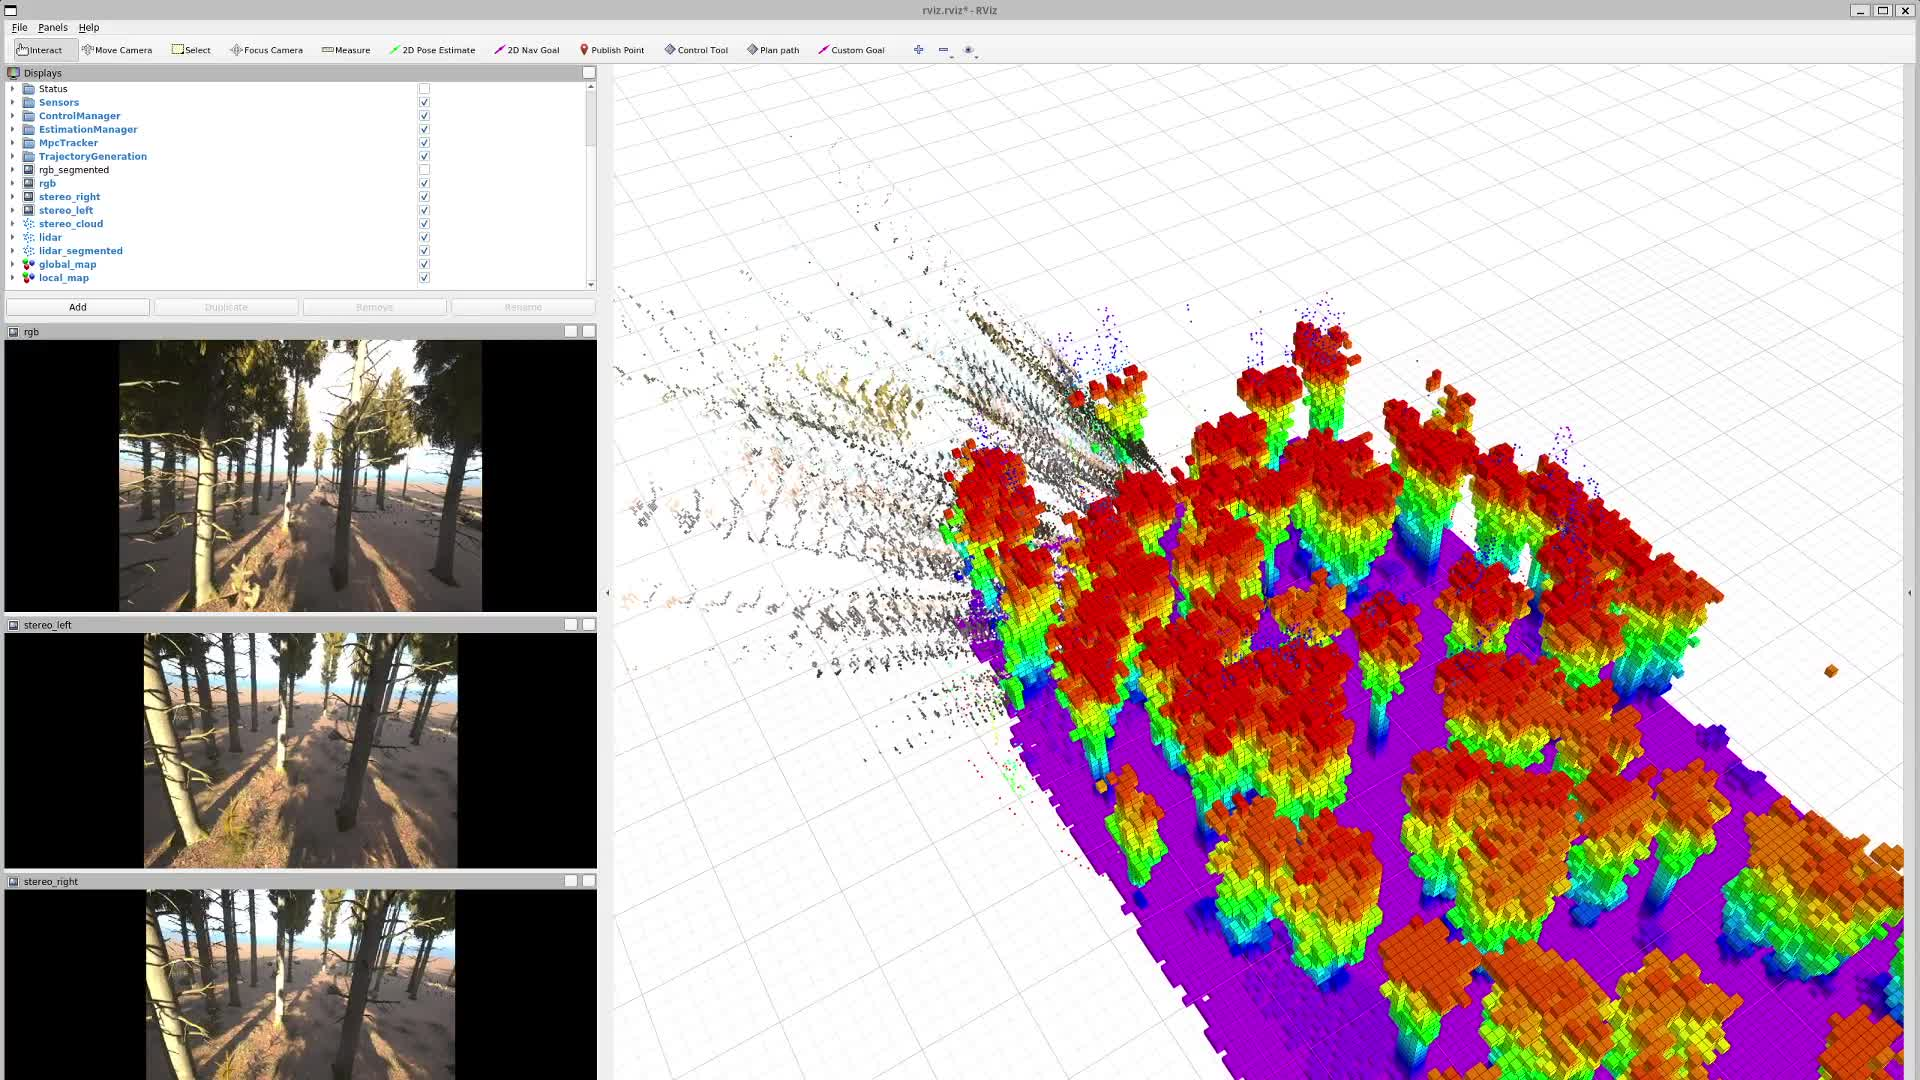
\includegraphics[width=0.8\textwidth]{fig/unreal_mapping_thumbnail.jpg}
        }{videos/unreal_mapping.mp4}\\
      \end{center}
    \end{block}

  \end{frame}

  %%}

  %%{ Precise Landing

  \begin{frame}
    \frametitle{Precise landing based on a marker}

    \begin{block}{Precise landing on an April tag}
      \begin{center}
        \mymovie[autostart,loop]{
          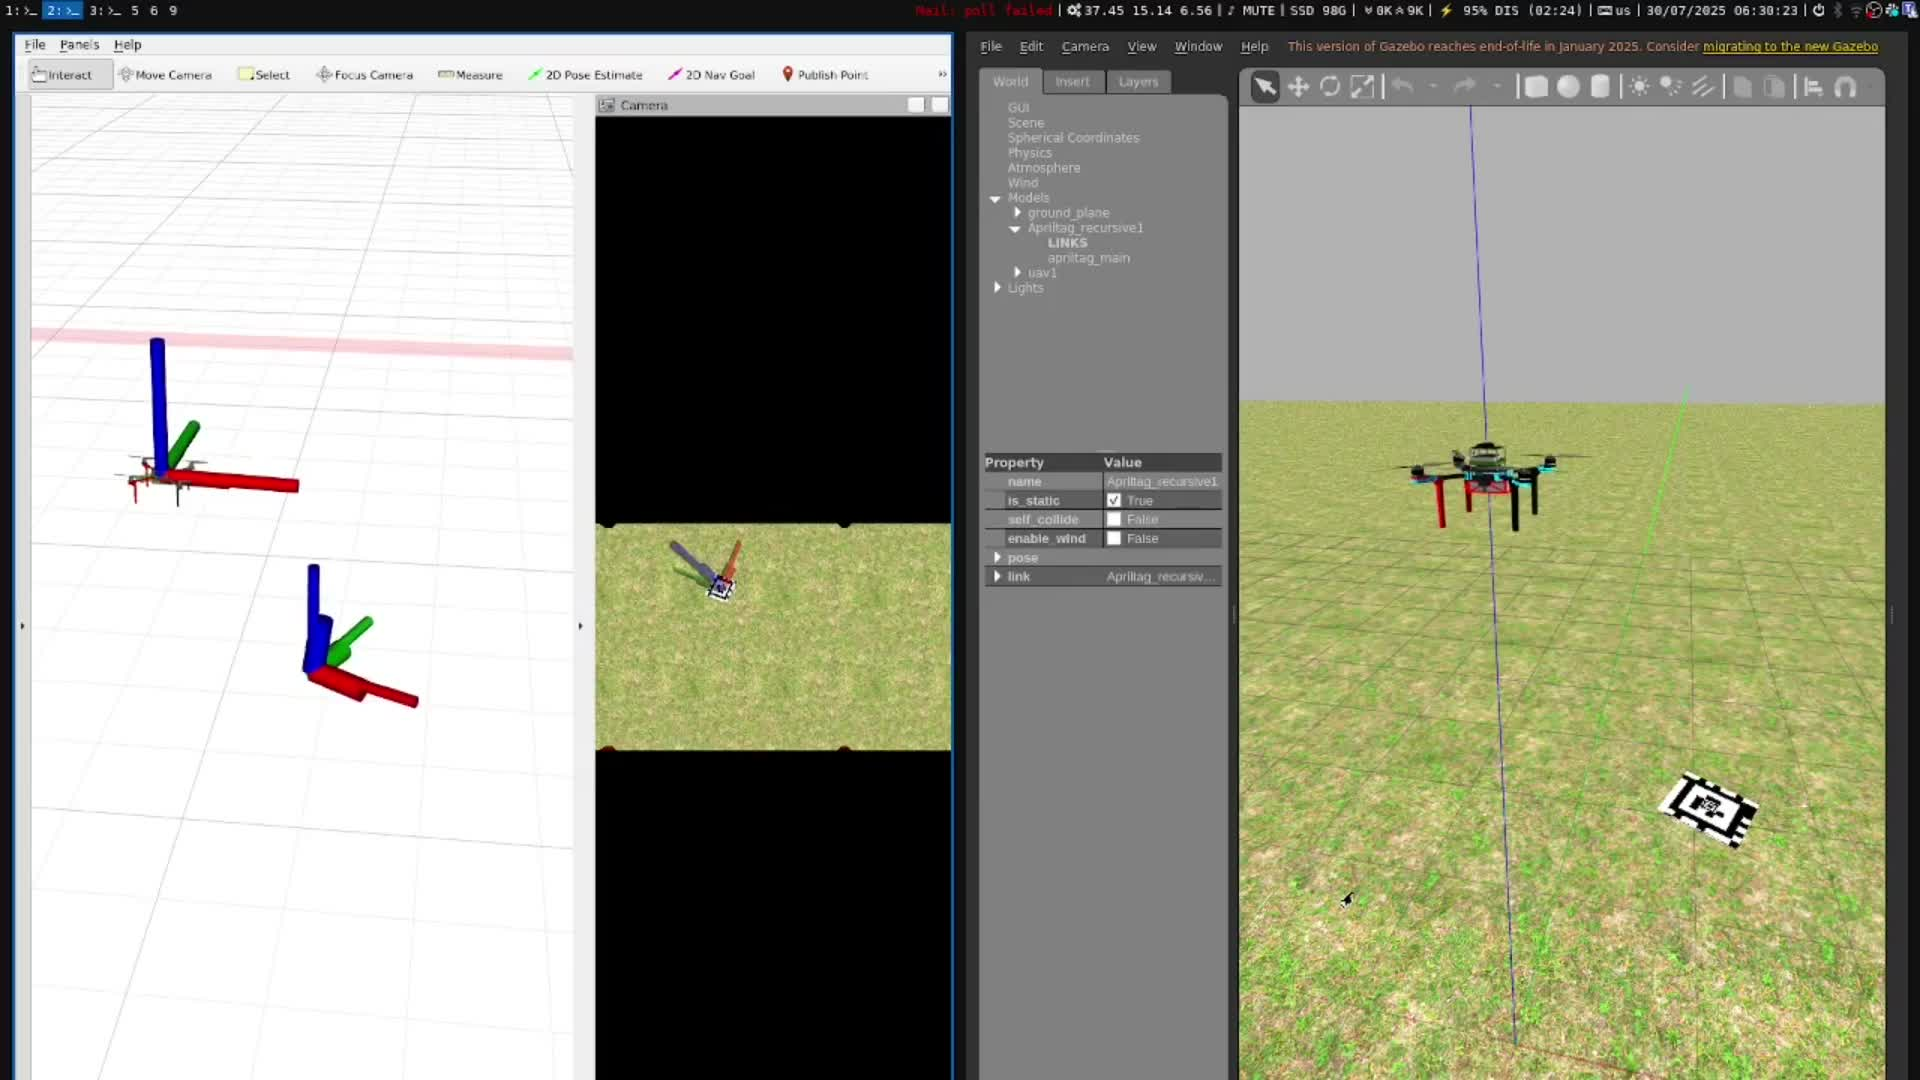
\includegraphics[width=0.8\textwidth]{fig/precise_landing_thumbnail.jpg}
        }{videos/precise_landing.mp4}\\
      \end{center}
    \end{block}

  \end{frame}

  %%}

%% | --------------------- Implementation --------------------- |

\section{MRS UAV System --- Implementation}

%%{ Our flying robots

\begin{frame}
  \frametitle{Our flying robots}

  \begin{columns}[c]

    \column{0.25\textwidth} % Left column and width

    \begin{figure}
      \centering
      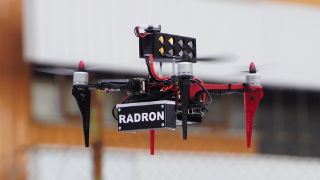
\includegraphics[width=1.0\textwidth]{./fig/uavs/f330_real.jpg}
    \end{figure}

    \vspace{-1em}

    \begin{figure}
      \centering
      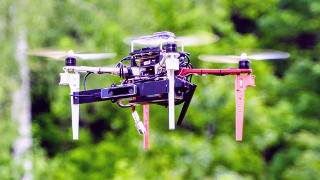
\includegraphics[width=1.0\textwidth]{./fig/uavs/f450_real.jpg}
    \end{figure}

    \vspace{-1em}

    \begin{figure}
      \centering
      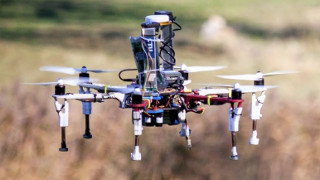
\includegraphics[width=1.0\textwidth]{./fig/uavs/f550_real.jpg}
    \end{figure}

    \column{0.25\textwidth} % Right column and width

    \begin{figure}
      \centering
      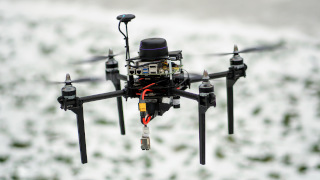
\includegraphics[width=1.0\textwidth]{./fig/uavs/x500_real.jpg}
    \end{figure}

    \vspace{-1em}

    \begin{figure}
      \centering
      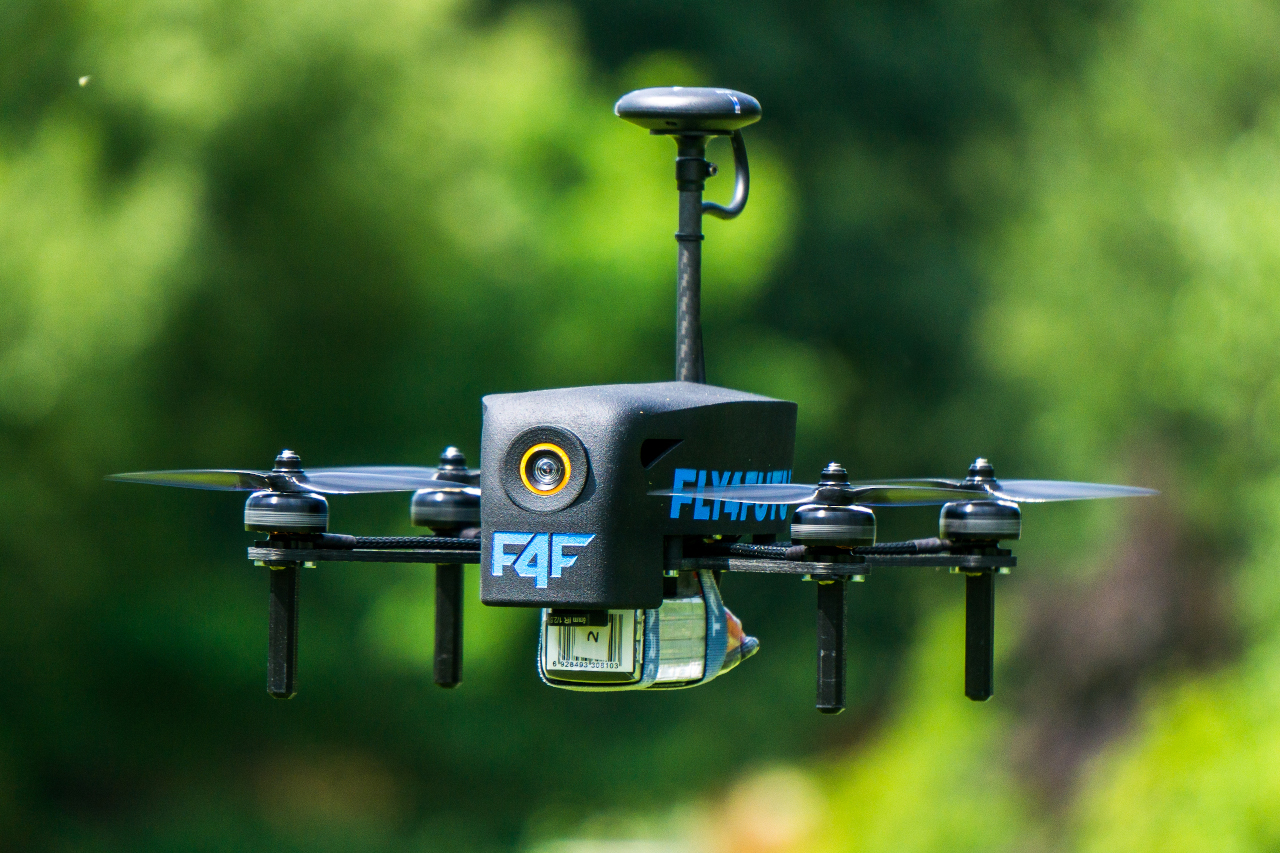
\includegraphics[width=1.0\textwidth]{./fig/uavs/ecodrone.jpg}
    \end{figure}

    \vspace{-1em}

    \begin{figure}
      \centering
      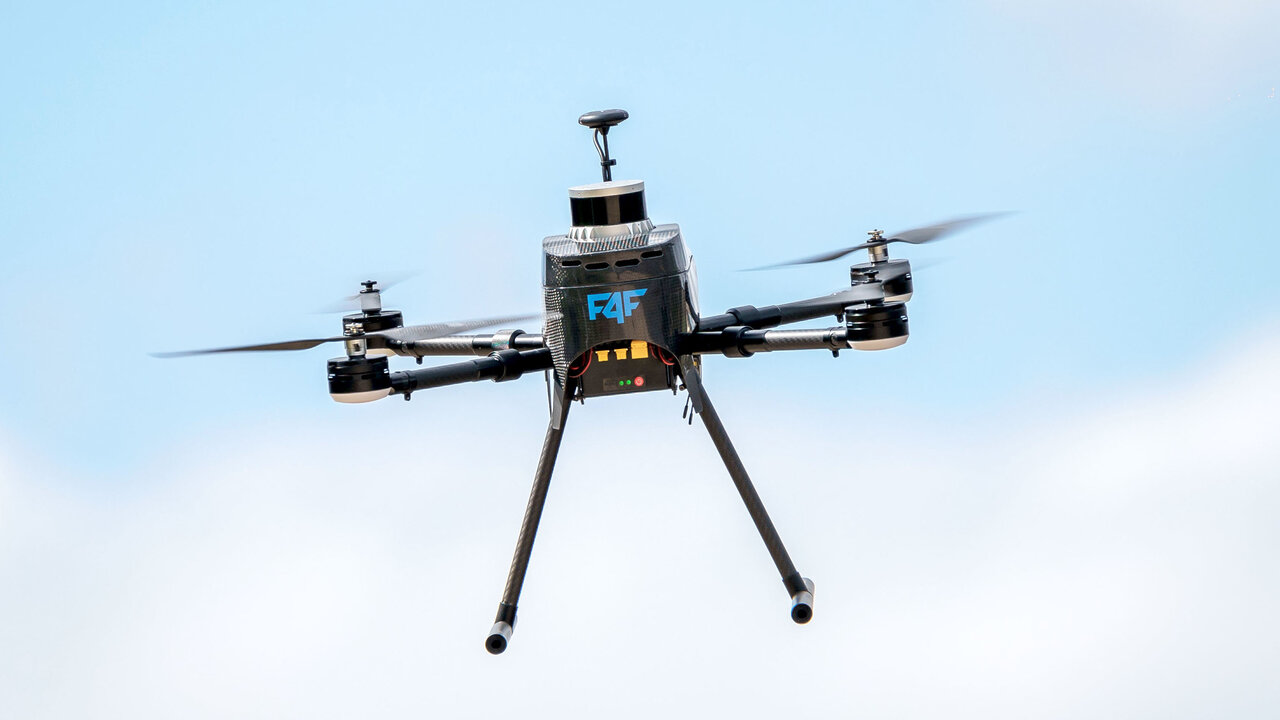
\includegraphics[width=1.0\textwidth]{./fig/uavs/t690_real.jpg}
    \end{figure}

    \column{0.25\textwidth} % Right column and width

    \begin{figure}
      \centering
      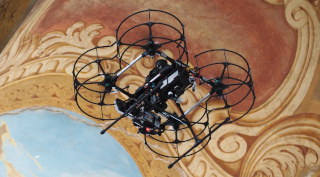
\includegraphics[width=1.0\textwidth]{./fig/uavs/naki_real.jpg}
    \end{figure}

    \vspace{-1em}

    \begin{figure}
      \centering
      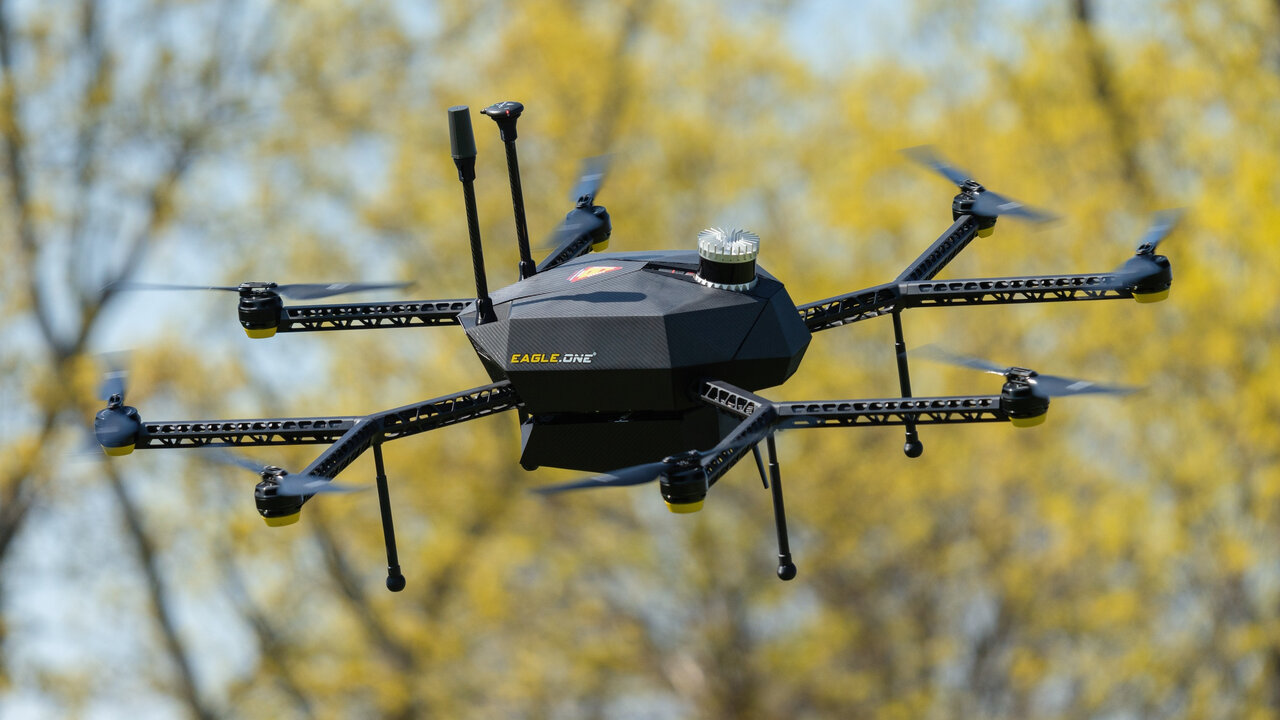
\includegraphics[width=1.0\textwidth]{./fig/uavs/eagle_real.jpg}
    \end{figure}

    \vspace{-1em}

    \begin{figure}
      \centering
      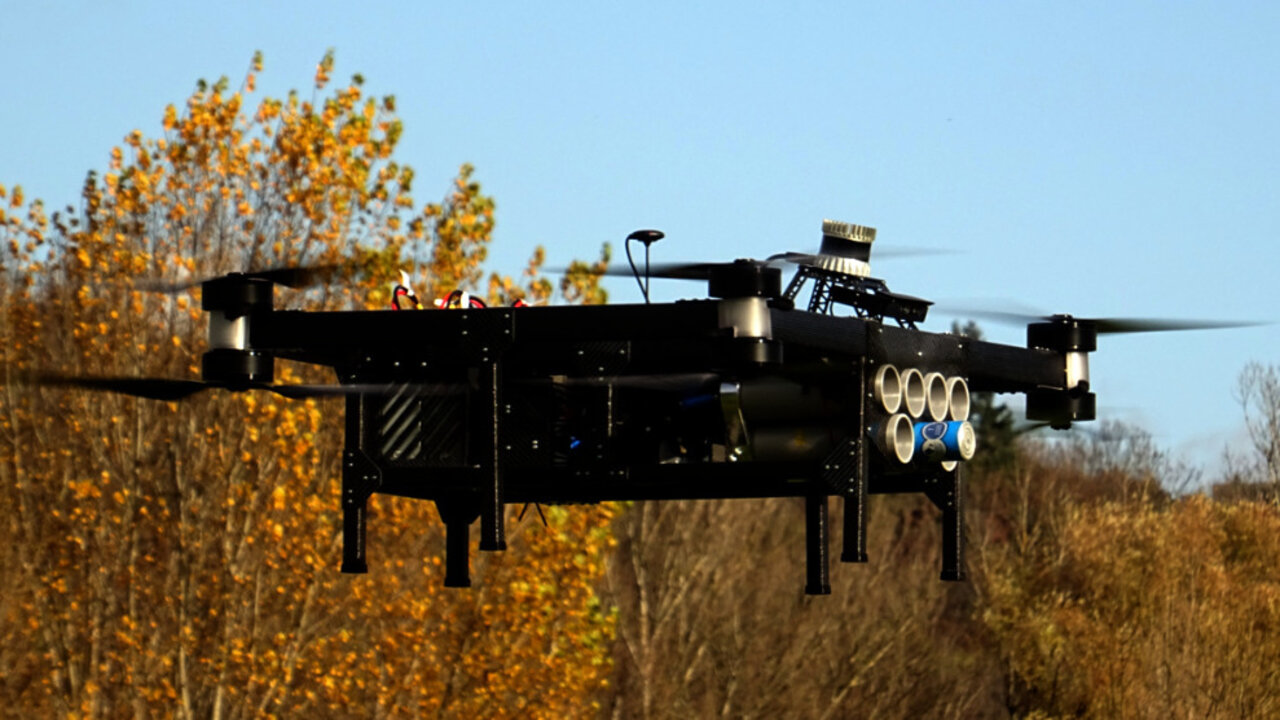
\includegraphics[width=1.0\textwidth]{./fig/uavs/dofec_real.jpg}
    \end{figure}

  \end{columns}

\end{frame}

%%}

%%%{ What's on your tool belt?

%\begin{frame}
%  \frametitle{What's on your tool belt?}

%  \begin{columns}[c]

%    \column{0.48\textwidth} % Left column and width
%    {\Huge Getting research done by:}
%    \begin{itemize}
%      \item using the tools provided by the community,
%      \item adapting tools provided by the community,
%      \item creating tools for yourself,
%      \item providing tools for the community.
%    \end{itemize}

%    \vspace{2em}

%    \only<2>{
%      \begin{center}
%        {\huge {\color{red} Automation}}
%      \end{center}
%    }

%    \column{0.48\textwidth} % Right column and width
%    \begin{figure}
%      \centering
%      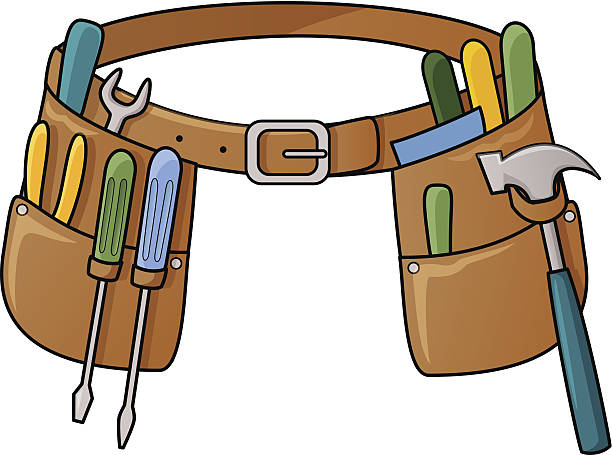
\includegraphics[width=1.0\textwidth]{./fig/tool_belt.jpg}
%    \end{figure}

%  \end{columns}

%\end{frame}

%%%}

%%{ Gazebo

\section{Gazebo}

\begin{frame}

  \frametitle{Gazebo/ROS simulation pipeline}

  \begin{columns}[c]

    \column{0.5\textwidth} % Left column and width
    \begin{figure}
      \centering
      
\includegraphics[width=0.5\textheight]{./fig/gazebo_logo.png}
    \end{figure}

    \column{0.5\textwidth} % Right column and width
    \only<2>{
      \begin{figure}
        \centering
        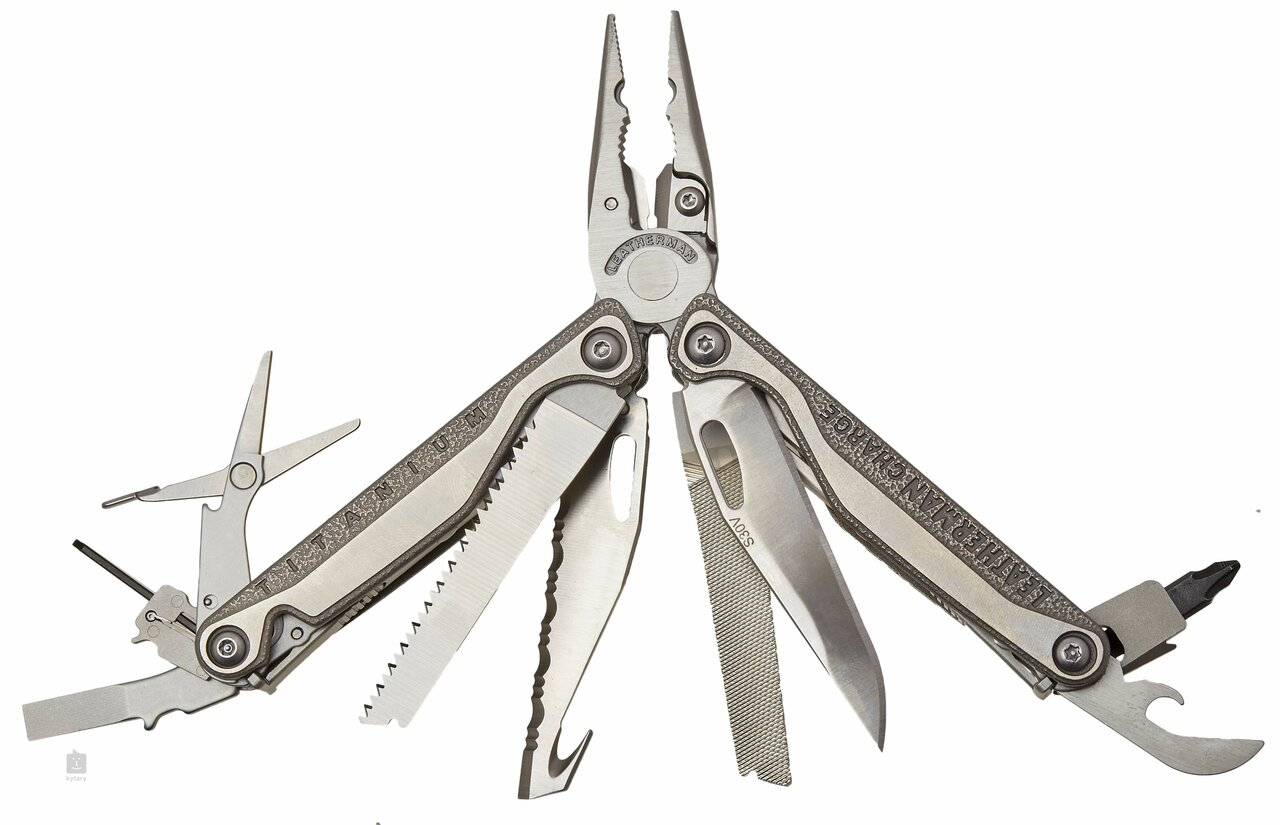
\includegraphics[width=0.8\textwidth]{./fig/leatherman.jpg}
      \end{figure}
    }

  \end{columns}

\end{frame}

%%}

%%{ Gazebo SITL

% \subsection{Baseline UAV spawning}

% \begin{frame}
%   \frametitle{Gazebo/ROS SITL - Common interaction of the components}

%   \begin{figure}
%     \centering
%     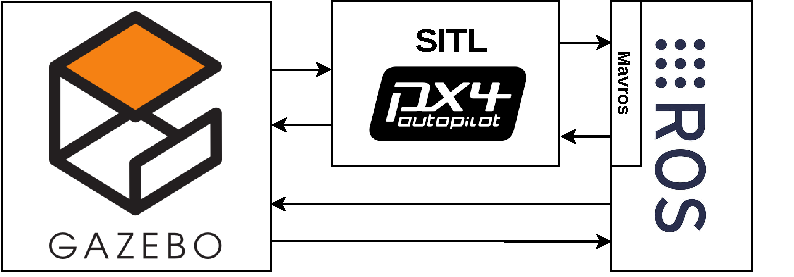
\includegraphics[width=1.0\textwidth]{./fig/schematics/sitl.pdf}
%   \end{figure}

% \end{frame}

%%}

%%%{ Gazebo Old spawning

%\begin{frame}
%  \frametitle{Gazebo/ROS PX4 traditional SITL spawning}

%  \only<1>{
%    
\includegraphics[width=1.0\textwidth]{./fig/schematics/gazebo_old_1.pdf}
%  }

%  \only<2>{
%    
\includegraphics[width=1.0\textwidth]{./fig/schematics/gazebo_old_2.pdf}
%  }

%  \only<3>{
%    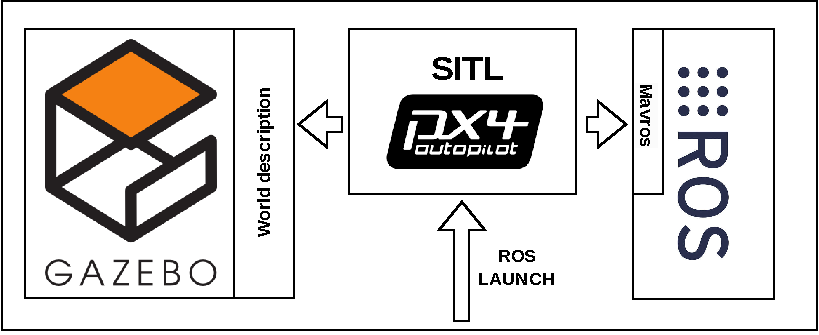
\includegraphics[width=1.0\textwidth]{./fig/schematics/gazebo_old_3.pdf}
%  }

%\end{frame}

%%%}

%%{ Sitl gazebo files

% \begin{frame}
%   \frametitle{Gazebo/ROS SITL Gazebo files}

%   \begin{itemize}
%     \item manual editing does not scale
%   \end{itemize}

%   \begin{figure}
%     \centering
%     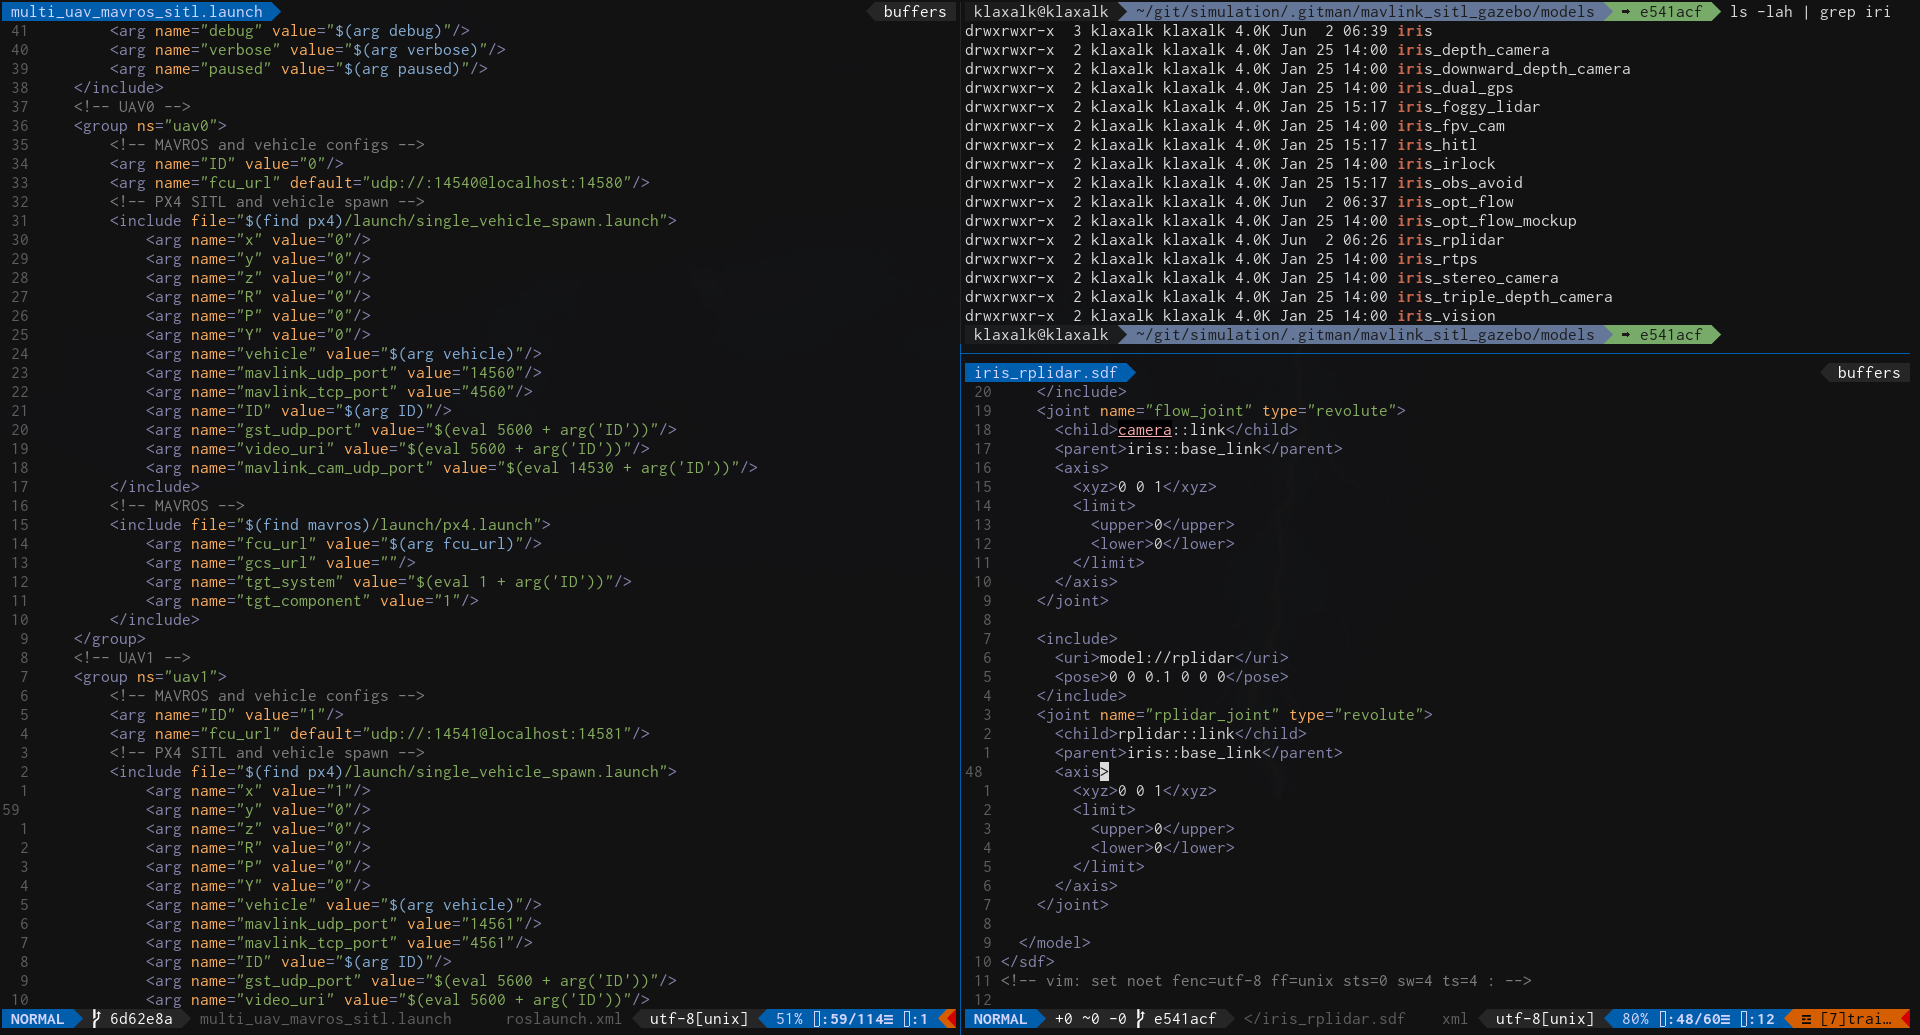
\includegraphics[width=0.85\textwidth]{./fig/sitl_gazebo_files.png}
%   \end{figure}

% \end{frame}

%%}

%%{ Gazebo MRS spawning

\subsection{MRS custom spawning}

\begin{frame}
  \frametitle{Gazebo/ROS MRS PX4 SITL spawning}

  \begin{itemize}
    \item scalable for any UAV configuration
  \end{itemize}

  % \only<1>{
  %   
\includegraphics[width=1.0\textwidth]{./fig/schematics/gazebo_mrs_1.pdf}
  % }

  % \only<2>{
  %   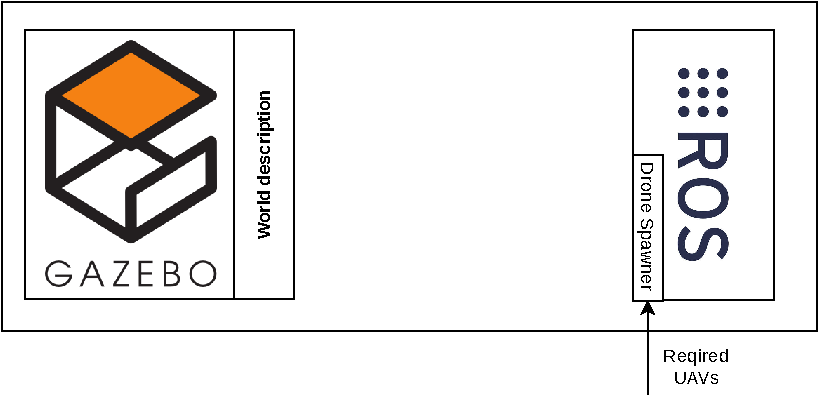
\includegraphics[width=1.0\textwidth]{./fig/schematics/gazebo_mrs_2.pdf}
  % }

  % \only<3>{
  %   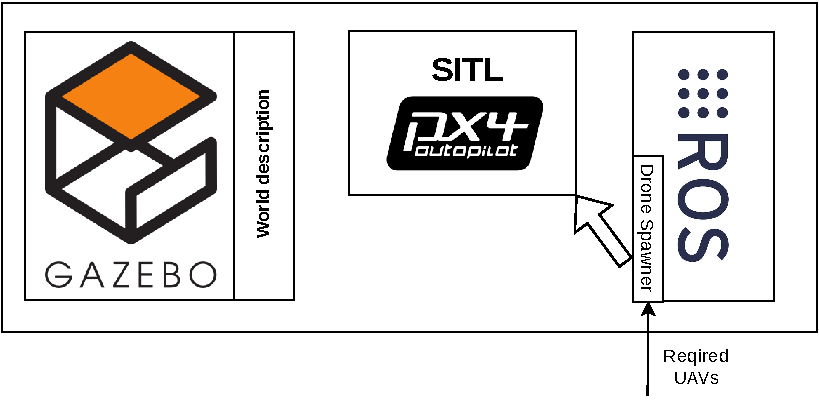
\includegraphics[width=1.0\textwidth]{./fig/schematics/gazebo_mrs_3.pdf}
  % }

  % \only<4>{
  %   \includegraphics[width=1.0\textwidth]{./fig/schematics/gazebo_mrs_4.pdf}
  % }

  \only<+>{
    \includegraphics[width=1.0\textwidth]{./fig/schematics/gazebo_mrs_5.pdf}
  }

  \only<+>{
    \includegraphics[width=1.0\textwidth]{./fig/schematics/gazebo_mrs_6.pdf}
  }

\end{frame}

%%}

%%{ Customizing the UAV payload

\begin{frame}
  \frametitle{Parametric UAV-payload customization}

  \begin{columns}[c]

    \column{0.48\textwidth} % Left column and width

    \vspace{-1em}

    \onslide<1->{
      \begin{block}{1. Definition of universal payloads}
        \begin{itemize}
          \item Payload models with plugins defined in a separate file.
        \end{itemize}
      \end{block}
    }

    \onslide<2->{
      \vspace{-0.5em}

      \begin{block}{2. Definition of platform-specific mounting points}
        \begin{itemize}
          \item Arbitrary placement and configuration of particular payload for particular platform.
        \end{itemize}
      \end{block}
    }

    \onslide<3>{
      \vspace{-0.5em}

      \begin{block}{3. Dynamic assembly of the final UAV sdf structure}
        \begin{itemize}
          \item The robot description file is assembled based on user's query.
          \item Any-to-any mapping between UAV frames and UAV payloads
          \item Queries are queued and executed in series.
        \end{itemize}
      \end{block}
    }

    \column{0.48\textwidth} % Right column and width

    \vspace{-1em}

    \only<1>{
      \vspace{-2em}

      \begin{figure}
        \includegraphics[width=1.0\textwidth]{./fig/component_snippets.png}
      \end{figure}
    }

    \only<2>{
      \vspace{-2em}

      \begin{figure}
        \includegraphics[width=1.0\textwidth]{./fig/f450_sdf.png}
      \end{figure}
    }

    \only<3>{
      \begin{block}{Bonus facts}
        \begin{itemize}
          \item Potential definition of sensor groups.
          \item Support for query parameters --- additional customization.
        \end{itemize}
      \end{block}

      \begin{block}{Spawning query}
        \texttt{rosservice call /mrs\_drone\_spawner/spawn "1 --x500 --pos 0 0 1 0 --enable-rangefinder --enable-realsense-front --enable-ouster model:=OS0-128 use\_gpu:=True"}
      \end{block}
    }

  \end{columns}

\end{frame}

%%}

%%%{ How about sensor transformations?

%\begin{frame}
%  \frametitle{What about sensor static transformations?}

%  \onslide<1->{
%    \huge Static tfs are specific to each sensors individual placement on UAV!
%  }

%  \onslide<2->{
%    \huge Only Gazebo knows them...
%  }

%  \vspace{1em}

%  \onslide<3->{
%    \begin{block}{\huge Solution:}
%      \large World plugin that listens to Gazebo tfs and republishes them as ROS tfs.
%    \end{block}
%  }

%\end{frame}

%%%}

%%{ Simulator UAVs

\begin{frame}
  \frametitle{Simulator UAVs}

  \begin{columns}[c]

    \column{0.48\textwidth} % Left column and width
    \includegraphics[width=1.0\textwidth]{./fig/simulator_uavs_1.jpg}

    \column{0.48\textwidth} % Right column and width
    \includegraphics[width=1.0\textwidth]{./fig/simulator_uavs_2.jpg}

  \end{columns}

\end{frame}

%%}

%%%{ Live demo

%\subsection{Spawner demo}

%\begin{frame}
%  \frametitle{Live demo!}

%  \begin{center}
%    \huge Live demo
%  \end{center}

%\end{frame}

%%%}

  %%{ MRS UAV System --- Gazebo simulation

  \begin{frame}
    \frametitle{MRS UAV System --- Gazebo simulation}

    \vspace{-0.33em}

    \includegraphics[width=1.0\textwidth]{./fig/thumbnail_simulation.jpg}

    \vspace{-0.3em}

    \begin{itemize}
      \item 7 UAV types: DJI f330, DJI f450, DJI f550, T-Motor x500, Tarot 650, T-drone m690, Fly4Future's RoboFly
    \end{itemize}

    \begin{columns}[c]

      \column{0.60\textwidth} % Left column and width

      \begin{block}{Available sensors}
        \begin{itemize}
          \item RGB camera: MatrixVision Bluefox, Mobius
          \item Stereo Cameras: Intel Realsense
          \item 1D LiDARs: Terabee Teraranger, Gamin Lite
          \item 2D LiDARs: Scanse Sweep, Garmin RPLidar
          \item 3D LiDARs: Velodyne Puck, Ouster
          \item Thermal cameras, UV cameras for UVDAR
        \end{itemize}
      \end{block}

      \column{0.35\textwidth} % Right column and width

      \begin{block}{Available actuation}
        \begin{itemize}
          \item magnetic gripper
          \item parachute
          \item water gun
        \end{itemize}
      \end{block}

    \end{columns}

    \begin{center}
      \url{http://github.com/ctu-mrs/mrs_uav_gazebo_simulation}
    \end{center}

  \end{frame}

  % \begin{frame}
  %   \frametitle{MRS UAV System --- Gazebo Simulation}

  %   \begin{block}{Realistic simulations of UAV grasping a brick}
  %     \begin{center}
  %       \mymovie[autostart,loop]{
  %         \includegraphics[width=0.8\textwidth]{fig/brick_grasping_simulated_thumbnail.jpg}
  %       }{videos/brick_grasping_simulated.mp4}\\
  %     \end{center}
  %   \end{block}

  % \end{frame}

  % \begin{frame}
  %   \frametitle{MRS UAV System --- Real world}

  %   \begin{block}{Real world UAV grasping a brick}
  %     \begin{center}
  %       \mymovie[autostart,loop]{
  %         \includegraphics[width=0.8\textwidth]{fig/brick_grasping_desert_thumbnail.jpg}
  %       }{videos/brick_grasping_desert.mp4}\\
  %     \end{center}
  %   \end{block}

  % \end{frame}

  %%}

%%{ Is one simulator enough

\begin{frame}
  \frametitle{Is one simulator enough?}

  \only<1>{
    \begin{center}
      \huge Is one simulator enough?
    \end{center}
  }

  \only<2>{
    \begin{block}{Large-scale swarms --- require high parallelization within the simulator}
      \begin{center}
        \mymovie[autostart,loop]{
          \includegraphics[width=0.75\textwidth]{./fig/swarm_14uavs_field_thumbnail.jpg}
        }{./videos/swarm_14uavs_field.mp4}
      \end{center}
    \end{block}
  }

  \only<3>{
    \begin{block}{High-fidelity visuals --- requires capable rendering engine}
      \begin{center}
        \mymovie[autostart,loop]{
          \includegraphics[width=0.60\textwidth]{./fig/ue5_example_thumbnail.jpg}
        }{./videos/ue5_example.mp4}
      \end{center}
    \end{block}
  }

  \only<4>{
    \begin{block}{CoppeliaSim --- Ease of use and deployment}
      \begin{center}
        \mymovie[autostart,loop]{
          \includegraphics[width=0.80\textwidth]{./fig/coppelia_thumbnail.jpg}
        }{./videos/coppelia.mp4}
      \end{center}
    \end{block}
  }

  \only<5->{
    \begin{center}
      \huge Is one simulator enough?
      \huge {\color{red} No}\\
      \huge Each simulator has pros and cons:
    \end{center}
  }

  \only<6->{
    \begin{columns}[c]

      \column{0.3\textwidth} % Left column and width
      \only<6->{
        \begin{figure}
          \includegraphics[width=1.0\textwidth]{./fig/leatherman.jpg}
        \end{figure}
      }

      \column{0.3\textwidth} % Right column and width
      \only<7->{
        \begin{figure}
          \includegraphics[width=1.0\textwidth]{./fig/inflatable_tools.jpg}
        \end{figure}
      }

      \column{0.3\textwidth} % Right column and width

      \only<8->{
        \begin{figure}
          \includegraphics[width=1.0\textwidth]{./fig/screw_drivers.jpg}
        \end{figure}
      }

    \end{columns}
  }

\end{frame}

%%}

%%{ How to interact with simulators

% \begin{frame}
%   \frametitle{How to interact with simulators}

%   \onslide<1->{
%     \huge How to interact with various simulators?
%   }

%   \onslide<2>{
%     \vspace{2em}

%     \huge How to interact with various hardware of UAV platforms?
%   }

% \end{frame}

%%}

%%{ MRS UAV System

% \begin{frame}
%   \frametitle{MRS UAV System --- the ``old vendor-locked-in'' system architecture}

%   \begin{figure}
%     \centering
%     \includegraphics[width=0.8\textwidth]{./fig/schematics/mrs_system_with_px4.pdf}
%   \end{figure}

%   \fullciteinbox{baca2021mrs}{}

% \end{frame}

%%}

%%{ Various requirements and features

% \begin{frame}
%   \frametitle{Various requirements and functionalities of UAV platforms}

%   \begin{columns}[c]

%     \column{0.48\textwidth} % Left column and width
%     \onslide<1->{
%       \begin{block}{UAV Inputs}
%         \begin{itemize}
%           \item attitude rate + throttle,
%           \item velocity + heading,
%           \item individual actuators,
%           \item etc.
%         \end{itemize}
%       \end{block}
%     }

%     \column{0.48\textwidth} % Right column and width
%     \onslide<2>{
%       \begin{block}{Provided data}
%         \begin{itemize}
%           \item IMU,
%           \item GNSS,
%           \item attitude,
%           \item velocity,
%         \end{itemize}
%       \end{block}
%     }

%   \end{columns}

% \end{frame}

%%}

%%{ Solution

% \begin{frame}
%   \frametitle{Solutions?}

%   \onslide<2->{
%     \begin{block}{Naive and the simplest solution at the beginning}
%       \begin{itemize}
%         \item Adding options and different configurations of your control system for each platform API.
%         \item {\color{green} low overhead in the beginning}
%         \item {\color{red} not scalable, hard-to-maintain, ties the system with dependencies}
%       \end{itemize}
%     \end{block}
%   }

%   \onslide<3>{
%     \begin{block}{Better solution for the long run}
%       \begin{itemize}
%         \item Add an \textbf{abstraction} layer
%         \item {\color{green} scales well, removes dependencies, provides isolation from particular technology}
%         \item {\color{red} introduces implementation and performance overhead}
%       \end{itemize}
%     \end{block}
%   }
% \end{frame}

%%}

%%{ What other simulators do we use?

% \begin{frame}
%   \frametitle{What other simulators?}

%   \begin{columns}[c]

%     \column{0.33\textwidth} % Left column and width
%     \begin{block}{Coppelia}
%       \begin{itemize}
%         \item Easy to use
%         \item Simple dependencies
%         \item {\color{red} bad multi-uav performance}
%       \end{itemize}
%     \end{block}

%     \column{0.65\textwidth} % Right column and width
%     \begin{center}
%       \mymovie[autostart,loop]{
%         \includegraphics[width=1.00\textwidth]{./fig/coppelia_thumbnail.jpg}
%       }{./videos/coppelia.mp4}
%     \end{center}

%   \end{columns}

% \end{frame}

%%}

%%{ Swarm of 400 UAVs

\begin{frame}
  \frametitle{The MRS Multirotor simulator --- swarm of 400 UAVs}

  \begin{block}{The MRS swarm simulator}
    \begin{center}
      \mymovie[autostart,loop]{
        \includegraphics[width=0.75\textwidth]{./fig/400_swarm_thumbnail.jpg}
      }{./videos/400_swarm.mp4}\\
    Video: \url{https://youtu.be/2UJ7aYaHOX0}
    \end{center}
  \end{block}

\end{frame}

%%}

%%{ MRS Multirotor simulator

\begin{frame}
  \frametitle{Custom dynamics simulation --- github.com/ctu-mrs/mrs\_multirotor\_simulator}

  \vspace{-1em}

  \begin{columns}[c]

    \column{0.48\textwidth} % Left column and width

    \begin{block}{MRS multirotor simulator}
      \begin{itemize}
        \item Full multirotor dynamics
        \item Embedded feedback controllers
        \item Fast C\texttt{++} ODE solver
        \item \textbf{header-only library --- {\color{red} intended for RL}}
        \item available ROS integration
        \item minimum external dependencies
        \item tightly integrated into the MRS system's core
      \end{itemize}
    \end{block}

    \column{0.48\textwidth} % Right column and width

    \begin{block}{Available control inputs}
      \small
      \begin{itemize}
        \item Position \& heading
        \item Velocity \& heading
        \item Velocity \& heading rate
        \item Acceleration \& heading
        \item Acceleration \& heading rate
        \item Attitude \& throttle
        \item Attitude rate \& throttle
        \item Control group \& throttle
        \item Individual actuators' throttle
      \end{itemize}
    \end{block}
  \end{columns}

  \begin{figure}
    \includegraphics[width=1.0\textwidth]{./fig/schematics/full_dynamics.png}
  \end{figure}

\end{frame}

%%}

%%{ FlightForge simulator

\begin{frame}
  \frametitle{FlightForge simulator (The MRS Multirotor + Unreal Engine 5)}

  \begin{columns}[c]

    \column{0.21\textwidth} % Left column and width

    \begin{itemize}
      \item RGB camera
      \item Stereo camera
      \item 3D LiDAR
      \item Ground truth segmentation in LiDAR and RGB
      \item Step-locked with our dynamics simulator (ROS)
    \end{itemize}

    \column{0.78\textwidth} % Right column and width

    \begin{center}
      \mymovie[autostart,loop]{
        \includegraphics[width=0.80\textwidth]{./fig/unreal_showcase_thumbnail.jpg}
      }{./videos/unreal_showcase.mp4}
    \end{center}

  \end{columns}

  \begin{block}{\centering \textbf{\url{https://github.com/ctu-mrs/mrs_uav_flightforge_simulator}}}
    \small \fullcite{capek2025flightforge}
  \end{block}

\end{frame}

%%}

%%{ mrs uav sytem HW api

\begin{frame}
  \frametitle{MRS UAV System --- hardware API}

  % \only<1>{
  %   \begin{figure}
  %     \centering
  %     \includegraphics[width=1.0\textwidth]{./fig/schematics/hw_api_1.pdf}
  %   \end{figure}
  % }

  % \only<2>{
  %   \begin{figure}
  %     \centering
  %     \includegraphics[width=1.0\textheight]{./fig/schematics/hw_api_2.pdf}
  %   \end{figure}
  % }

  % \only<3>{
  %   \begin{figure}
  %     \centering
  %     \includegraphics[width=1.0\textwidth]{./fig/schematics/hw_api_3.pdf}
  %   \end{figure}
  % }

  \begin{block}{Interfacing with any simulator or flight controller}

    \only<1>{
      \begin{figure}
        \centering
        \includegraphics[width=0.9\textwidth]{./fig/schematics/hw_api_3.pdf}
      \end{figure}
    }

    \only<2>{
    \begin{figure}
      \centering
      \includegraphics[width=0.9\textwidth]{./fig/schematics/hw_api_4.pdf}
    \end{figure}
    }
  \end{block}

\end{frame}

%%}

%%{ HW API plugin api

\subsection{General flight controller}

\begin{frame}
  \frametitle{HW API's API --- Definition of a general flight controller}

  \begin{columns}[c]

    \column{0.48\textwidth} % Left column and width
    \begin{block}{Information provided}
      Subset of the following:
      \begin{itemize}
        \item IMU
        \item GNSS
        \item RTK GNSS
        \item Magnetometer
        \item AMSL measurement
        \item Ground truth pose
        \item Height measurement
        \item Angular rate
        \item RC channels
        \item Velocity
        \item Orientation
        \item 3D Pose
      \end{itemize}
    \end{block}

    \column{0.48\textwidth} % Right column and width
    \begin{block}{Control input accepted}
      Subset of the following:
      \begin{itemize}
        \item Position \& heading
        \item Velocity \& heading
        \item Velocity \& heading rate
        \item Acceleration \& heading
        \item Acceleration \& heading rate
        \item Attitude \& throttle
        \item Attitude rate \& throttle
        \item Control group \& throttle
        \item Individual actuators' throttle
      \end{itemize}
    \end{block}

  \end{columns}

\end{frame}

%%}

%%{ MRS UAV System

\begin{frame}
  \frametitle{MRS UAV System --- all open-source}

  \begin{figure}
    \centering
    \includegraphics[width=0.7\textwidth]{./fig/github.png}
    \huge {\color{blue} http://github.com/ctu-mrs}
  \end{figure}

\end{frame}

%%}

%%{ Sources

\begin{frame}
  \frametitle{How to get the MRS UAV System \& Sources}

  \begin{block}{Native installation over ROS Noetic}
    \texttt{curl https://ctu-mrs.github.io/ppa-stable/add\_ppa.sh | bash}\\
    \texttt{sudo apt install ros-noetic-mrs-uav-system-full}
  \end{block}

  \begin{block}{Apptainer container system + container wrapper}
    \begin{center}
      \large {\color{blue} http://github.com/ctu-mrs/mrs\_apptainer}
    \end{center}
  \end{block}

  \begin{block}{Docker containers}
    \begin{center}
      \large {\color{blue} http://github.com/ctu-mrs/mrs\_docker}
    \end{center}
  \end{block}

  \begin{block}{Sources}
    \begin{center}
      \large {\color{blue} http://github.com/ctu-mrs/mrs\_uav\_system}
    \end{center}
  \end{block}

  \begin{block}{Documentation}
    \begin{center}
      \large {\color{blue} https://ctu-mrs.github.io/docs/1.5.0/introduction/}
    \end{center}
  \end{block}

\end{frame}

%%}

%%{ ROS2

\begin{frame}
  \frametitle{Transition to ROS2 - ROS2 Jazzy (Ubuntu 24.04)}

\begin{columns}[c]

\column{0.48\textwidth} % Right column and width

\begin{block}{Problematic at best}
  \begin{itemize}
    \item realtime issues with DDSs ($\implies$ Zenoh (2024))
    \item buggy client libraries (executors, timers)
    \item design regressions all over the board
    \item performance significantly worse than ROS1
  \end{itemize}
\end{block}

\begin{block}{State of transition}
  \begin{center}
    \includegraphics[width=0.5\textwidth]{./fig/rros2_diagram.png}
    \url{https://ctu-mrs.github.io/ros2_obsidian_knowledgebase/main_canvas.html}
  \end{center}
\end{block}

\column{0.48\textwidth} % Left column and width
\begin{block}{Available in ROS2}
  \begin{itemize}
    \item MRS UAV Core
    \item PX4 HW API
    \item MRS Multirotor sim
    \item FlightForge sim
    \item some sensor drivers
  \end{itemize}
\end{block}

\begin{block}{To be done}
  \begin{itemize}
    \item {\color{red} MRS Gazebo stack}
    \item {\color{red} GNSS-denied flight (LiDAR, VIO)}
    \item {\color{red} Octomap Mapping \& Planning}
    \item {\color{red} Precise landing}
    \item {\color{red} Pointcloud utils}
    \item {\color{red} Lot of QoL utilities}
    \item {\color{red} \textbf{Documentation}}
  \end{itemize}
\end{block}


\end{columns}

\end{frame}

%%}

%%{ Sources

\begin{frame}
  \frametitle{How to get the MRS UAV System in ROS2 \& Sources}

  \begin{block}{Native installation over ROS2 Jazzy}
    \texttt{curl https://ctu-mrs.github.io/ppa2-stable/add\_ppa.sh | bash}\\
    \texttt{sudo apt install ros-jazzy-mrs-uav-system-full}
  \end{block}

  \begin{block}{Sources}
    \begin{center}
      \large {\color{blue} http://github.com/ctu-mrs/mrs\_uav\_system/tree/ros2}
    \end{center}
  \end{block}

  \begin{block}{Documentation}
    \begin{center}
      \large {\color{blue} https://ctu-mrs.github.io/docs/2.0.0/introduction/}
    \end{center}
  \end{block}

\end{frame}

%%}

  %%{ MRS wiki

  % \begin{frame}
  %   \frametitle{MRS UAV System wiki}
  %   \begin{figure}
  %     \vspace{-1em}
  %     \caption*{\url{http://ctu-mrs.github.io}}
  %     \includegraphics[width=0.7\textwidth]{fig/wiki.png}
  %   \end{figure}

  % \end{frame}

  %%}

  %%{ MRS Cheat Sheet

  % \begin{frame}
  %   \frametitle{The MRS Cheat Sheet}
  %   \vspace{-1.0em}
  %   \begin{figure}
  %     \caption*{\url{http://github.com/ctu-mrs/mrs_cheatsheet}}
  %     \vspace{-0.5em}
  %     \includegraphics[width=0.8\textwidth]{fig/mrs_cheatsheet.png}
  %   \end{figure}
  % \end{frame}

  %%}

%%{ Conclusion

\begin{frame}
  \frametitle{Conclusions}

  \begin{center}
    \huge Thanks for your attention\\
  \end{center}

  \begin{block}{Download pdf of this presentation}
    \centering
    \Large\url{https://github.com/ctu-mrs/presentation_mrs_uav_system}
  \end{block}

  \begin{block}{My profile}
    \centering
    \Large\url{http://mrs.felk.cvut.cz/people/tomas-baca}
  \end{block}

  \begin{block}{\centering \textbf{Cite the MRS UAV System if you use it for your research}}
    \small \fullcite{baca2021mrs}
  \end{block}

\end{frame}

%%}

%%{ References

\DeclareCiteCommand{\fullcite}
{\usebibmacro{prenote}}
{\clearfield{addendum}%
  \usedriver
  {\defcounter{minnames}{6}%
  \defcounter{maxnames}{6}}
{\thefield{entrytype}}}
{\multicitedelim}
{\usebibmacro{postnote}}

\begin{frame}[allowframebreaks]
  \frametitle{References}
  \tiny{
    \printbibliography[heading=none,title={}]
  }
\end{frame}

%%}

\end{document}
